\documentclass[a4paper]{report}

\usepackage{geometry}
\geometry{textwidth=15.75cm, textheight=23.4cm, marginratio={5:5,5:7}}

\usepackage[page]{totalcount}

\usepackage{fancyhdr}
\pagestyle{fancy}

\rfoot{\fancyplain{}{CONNOR M\textsuperscript{c}LAUGHLIN}}
\rhead{\fancyplain{}{\thepage\ of \totalpages}}
\lhead{\fancyplain{}{\leftmark}}
\lfoot{\fancyplain{}{GRADUATE APPRENTICESHIP SOFTWARE ENGINEERING}}

\fancyhf[FC]{} % Disable page numbers in footer center.

\usepackage{amsmath} % Math equations
\usepackage{booktabs} % Better looking tables
\usepackage[RPvoltages]{circuitikz} % The circuit diagrams in CANS
\usepackage{float} % Used to force listings to have H placement
\usepackage{microtype} % Slightly better text layouts
\usepackage{minted} % Code
\usepackage[simplified]{pgf-umlcd} % Used to have UML diagrams in TSI
\usepackage[binary-units=true]{siunitx} % Units
\usepackage{tabularx} % Column types
\usepackage{tcolorbox} % The note box

\usepackage{enumitem}
\setlist{itemsep=0.5\itemsep}

\usepackage{hyperref}
\hypersetup{
    colorlinks,
    citecolor=black,
    filecolor=black,
    linkcolor=black,
    urlcolor=black
}

\usepackage{pifont}
\newcommand{\cmark}{\ding{51}}%
\newcommand{\xmark}{\ding{55}}%

\newenvironment{note} {
    \begin{tcolorbox}[title=Note]
 } {
     \end{tcolorbox}
 }

\begin{document}
\tableofcontents
\part{Semester One (2020-11-02)}
\chapter{How To Learn A New Language}
\section{Session One}\label{sub:session_one}

\subsection{Sprint One}\label{ssub:sprint_one}

\begin{itemize}
    \item First half is variables, loops and other basic programming constructs
    \item The second half is more advanced with object oriented programming
\end{itemize}

\begin{note}
    Overall the course could seem very easy, by Christmas, though, it will not.
\end{note}

\subsection{The Workplace}\label{ssub:the_workplace}

When back in the workplace, we will get tasks, don't stress about these too much --- if work deadlines are too tight, don't worry.
Learning logs will be useful for report writing.
You should take note of examples of university work found will at work.

Barclay's people are all just doing busy work --- nobody has done any programming yet and they started in August 2020. Because of this, my team all have no programming experience making me the designated experienced developer.

\section{Session Two}\label{sub:session_2_types}

\subsection{Types}\label{ssub:types}

\emph{Primitive types} are ones that cannot be broken down (\mintinline{c}{int}, \mintinline{c}{char}, \mintinline{c}{long}).
\emph{Composite types} can be broken down (array, class and sometimes strings are \mintinline{c}{char[]}s)

\begin{note}
	In most old languages (like C, C++), booleans are often represented by just a \(1\) or  \(0\).
	Also, strings are often just stored as an array of ASCII codes, Python is an exception where \mintinline{c}{chars} are just strings with length 1
\end{note}

\subsection{Learning Logs}\label{ssub:learning_logs}

A final workplace report worth \(25\%\) is due 2021-03-01.
\begin{itemize}
	\item Reflect and show what was learned at work.
	\item Should be about \(1500\) words in length.
	\item Should include a critical evaluation of the programming practices encountered.
	\item Should include examples of programming concepts covered in HTLANL (inheritance, scope, etc.).
	\item \textbf{What have I learned?}
\end{itemize}

\subsection{Academic Writing}\label{ssub:academic_writing}

On Moodle there is a basic introduction, phrase bank and a like to LEADS (a university program to help with academic writing).

Reflective writing is evidence of reflective thinking.
Reflective thinking helps to reinforce what we have learned.

Reflective writing is generally a more relaxed form of writing where you can write in first person (I, me, we).

Reflective writing should aim to look back at an event (\emph{description}), analyse and explain the event (\emph{interpretation}) and decide what this means for me in the future (\emph{outcome}).

\begin{note}
	When describing a theory or model, use present tense since the theory or model is still the same.
	When talking about events, use past tense since the events happened in the past.
\end{note}


\section{Section Three}\label{sub:section_three}

\subsection{Statements}\label{ssub:statements}

Statements are sequences of code that do something.
A program is a sequence of statements.
All expressions (\mintinline{python}{1+1}) are valid statements.

Assignment statements are a special type of statement:

\begin{itemize}
    \item They bind a value to a name.
    \item They bind the right hand side value to the left hand side value.
    \item Usually \mintinline{python}{=} symbol is used, but some languages use \mintinline{pascal}{:=} (Pascal) and \mintinline{r}{<-} (R).
\end{itemize}

\subsubsection{Expressions}\label{ssub:expressions}

Expressions don't necessarily have to have any effect.

\begin{itemize}
    \item \mintinline{python}{x + 5}
    \item \mintinline{python}{fn(32 * age) > 0}
\end{itemize}

\subsubsection{Operators}\label{ssub:operators}

Operators do a thing to a variable.
They are used in format: operand, operator, operand and they can often do different things in different contexts.

\subsubsection{Mathematical operators}\label{ssub:mathematical-operators}

\begin{itemize}
    \item \mintinline{python}{+}, \mintinline{python}{-}, \mintinline{python}{*}, \mintinline{python}{/}
    \item \mintinline{python}{**} and \mintinline{haskell}{exp} are for powers
    \item \mintinline{c}{%}, \mintinline{haskell}{rem} and \mintinline{haskell}{mod} are for modulus (remainder)
\end{itemize}

\subsubsection{Boolean Operators:}\label{ssub:boolean-operators}

\begin{itemize}
    \item \mintinline{python}{not} flips the expression
    \item \mintinline{python}{or} evaluates \mintinline{java}{true} if either operand is \mintinline{java}{true}.
    \item \mintinline{python}{and} evaluates \mintinline{java}{true} if both operands are \mintinline{java}{true}.
\end{itemize}

\subsubsection{Operator Overloading}\label{ssub:operator-overloading}

\begin{itemize}
    \item One operator can have different meanings depending on context:
        \begin{itemize}
            \item \mintinline{python}{"5" + "6" = "56"}
            \item \mintinline{python}{5 + 6 = 11}
        \end{itemize}
    \item Most languages don't allow the creation of custom overloaded operators (C is a notable exception)
\end{itemize}

\subsubsection{Precedence}\label{ssub:precedence}

\begin{itemize}
    \item Largely follows BODMAS
        \begin{minted}{python}
            x = 2 + 3 * 4
            x = 2 + 12
            x = 14
        \end{minted}
\end{itemize}

\subsection{Typing}\label{sub:typing}

Before an operator's operation can be performed, the type must be known.
Some type checkers happen at runtime, others at compile time depending on language.

\subsubsection{Static Typing}\label{ssub:static-typing}

\begin{itemize}
    \item A variable only ever has one type (a \mintinline{c}{long} will always be a \mintinline{c}{long}).
    \item Types can be set or inferred by the compiler.
    \item All operands and types are checked at compile time
\end{itemize}

\subsubsection{Dynamic Typing}\label{ssub:dynamic-typing}

\begin{itemize}
    \item Variables have no type, so values (which do have types) can be assigned to any variables.
    \item Operands and types are checked at runtime.
\end{itemize}

\subsubsection{Duck Typing}\label{ssub:duck-typing}

\begin{itemize}
    \item ``If a value looks like a certain type, acts like a certain type and talks like a certain type, then it is that type.''
    \item The language tries to do exactly what the programmer asks with the data given.
\end{itemize}

\subsubsection{Errors}\label{sub:errors}

\begin{itemize}
    \item You can only ever compare two comparable types. For example, in Python: \mintinline{python}{1 < True == False}.
\end{itemize}

\subsubsection{Type Conversions}\label{ssub:type-conversions}

\begin{itemize}
    \item Implicit:
        \begin{itemize}
            \item Happens automagically depending on context.
            \item For example: \mintinline{c}{int num = 123456789; long big = num}
        \end{itemize}
    \item Explicit (\emph{casting}):
        \begin{itemize}
            \item The programmer manually changes the types.
            \item For example: \mintinline{python}{int(n)}, \mintinline{typescript}{n as int}, \mintinline{c}{(int)n}
        \end{itemize}
\end{itemize}

\section{Session Four}\label{sec:session_four}

\subsection{Control}\label{sub:control}

Control allows you to chose which path to follow based on conditions.
A branch is somewhere the code can follow \(>1\) path.

\subsubsection{The if statement}\label{ssub:the-if-statement}

This is the very simplest type of branching.
\begin{highlight}{Python if statements}
    \begin{code}{python}
        if x:
        branch_one()
        if y:
        branch_two()
    \end{code}
\end{highlight}

\subsubsection{The else if statement}\label{ssub:the-else-if-statement}

One of the two paths are always followed.
\begin{highlight}{The Python else if statement}
    \begin{code}{python}
        if x:
        branch_one()
        else:
        branch_two()
    \end{code}
\end{highlight}

\subsubsection{The elif statement}\label{ssub:the-elif-statement}

\begin{itemize}
    \item Can handle more than just two outcomes.
    \item Could also be done with just lots of \mintinline{python}{if} statements, this is nasty and hard to read.
\end{itemize}

\begin{note}
    Switch and case statements can also handle more than one branch too.
\end{note}

\subsection{Iteration}\label{sub:iteration}

Repeating code is what makes computers powerful.
The key thing about looping is you do the same thing on different data.

\subsubsection{Definite Iteration}\label{ssub:definite-iteration}

\begin{itemize}
    \item Loop a certain number of times.
    \item Usually done with a \mintinline{python}{for} keyword.
\end{itemize}

\subsubsection{Nested Loops}\label{ssub:nested-loops}

\begin{itemize}
    \item One loop inside of another.
    \item Too many levels of looping is hard to read and slow.
\end{itemize}

\subsubsection{Indefinite Iteration}\label{ssub:indefinite-iteration}

\begin{itemize}
    \item Continues until some condition is met.
    \item Usually done with the \mintinline{python}{while} keyword.
    \item If the condition is \mintinline{java}{true}, the loop continues, otherwise it stops.
    \item Generally worse than definite loops.
    \item Use indefinite loops only when you don't know how many iterations there will be.
\end{itemize}

\section{Session Five}\label{sec:session_five}

\subsection{Subprograms}\label{sub:subprograms}

A \emph{subprogram} is a sequence of statements that can be called more than once (they are named blocks of code).
Subprograms often return a value which allows the subprogram to give feedback.
Sometimes these are called \emph{subroutines}, \emph{procedures}, \emph{functions} or \emph{methods}.
Subprograms temporarily reroute the flow of execution with isolated local variables and control the flow of data with arguments and returns.

\subsubsection{Return}\label{ssub:return}

Gives control back to the calling code from any point inside a function (even half way through).
If return is skipped, execution will end at the end of the code block.

\subsubsection{Call Stack}\label{ssub:call_stack}

Most languages have a stack of calls so that it always knows where code should return to.
When a function is called, it puts the point to return to onto the stack.
When a function returns again, it pops off the function and returns back to the point.

\subsubsection{Parametrisation}\label{ssub:parameterisation}

Functions are only really useful if they can be called with different data.
This is why we parametrise the functions to send data from the calling code.
\emph{Parameters} are the received data.
\emph{Arguments} are passed in.
Parameters are always required, but may be given a default value so they aren't need to be passed in every time.

\subsubsection{Why do we use functions?}\label{ssub:why_do_we_use_functions_}

\paragraph{Decomposition}\label{par:decomposition}

Makes code more readable and manageable.

\paragraph{Isolation}\label{par:isolation}

Isolate variables used in one chunk from those in another.

\paragraph{Abstraction}\label{par:abstraction}

Create a general function that can be used in many places for different problems.

\paragraph{Laziness}\label{par:laziness}

They can eliminate boring, repetitive tasks.
This is sometimes called \emph{generalisation} and is often done through abstraction. % link here

\paragraph{Remove repetition}\label{par:remove_repetition}

Repetition makes it very easy to make copy-paste mistakes and makes code harder to read.

\paragraph{Code sharing}\label{par:code_sharing}

Code in functions is far easier to share with other people if it is in chunks already.

\paragraph{Control the Effects}\label{par:control_the_effects}

Code in functions only affects local variables so there is a smaller risk of it breaking something outside.

\section{Session Six}\label{sec:session_six}

\subsection{Work-based Task}\label{sub:work_based_task}

Ask someone how they go about learning a new programming language or learning something new about a language they already know.

\subsection{Scope}\label{sub:scope}

Creating new variables inside of functions creates ones that are only available inside of that function named \emph{local variables}.
``Each function has its own workspace.''
Local variables are not persisted across calls.

\subsubsection{Global Scope}\label{ssub:global_scope}

These are variables outside of a function which are visible to all code.
Some languages don't really have global variables (C\# and Java just have \mintinline{java}{static}) and in Python, globals are read only by default to protect from accidental writes in local scopes (use \mintinline{python}{global} to write to them).

\subsubsection{Shadowing}\label{ssub:shadowing}

Local variables can shadow a global making it inaccessible.
In Python \mintinline{python}{global} must be used to edit globals in local scopes.

\subsubsection{Evils of Globalisation}\label{ssub:evils_of_glovalisation}

\emph{Globalisation} is generally considered bad practice because it makes functions rely on each other and variables can be changed accidentally leading to unintended behaviour.

\subsection{Recursion}\label{sub:recursion}

\emph{Recursion} is when a function calls itself.
This is an alternative to \mintinline{python}{while} and \mintinline{python}{for} loops.
Some problems can be solved by calling the same function on the data returned from last time.
eg. Fibonacci sequences, fractals, binary trees, sorts.


\section{Session Seven}\label{sec:session_seven}

\subsection{Data Structures}\label{sub:data_structures}

Organising data into structures is important.
Most languages have many built in data structures.
\emph{Data structures} are sometimes called \emph{composite data types} instead.
eg. Lists (arrays), dictionaries (hash maps), tuple (records).

\subsubsection{Lists (Python)}\label{ssub:lists_python_}

Python lists are dynamically sized meaning elements can be added or removed without changing the size unlike in C, for example, where an array has a fixed size.
Python lists are dynamically typed meaning that one list can have many different types of data.
The literal syntax (\mintinline{python}{a = [1, 2, 3, 4, 5, 6]}) can be used to declare and initialise a list in one line.

The \mintinline{python}{len()} function will return the number items in a list. eg. \mintinline{python}{len([1, 2, 3, 4, 5, 6]) == 6}.

To access an individual element in the list, use the \mintinline{python}{items[index]} syntax.
Lists can also be iterated over using a \mintinline{python}{for} loop: \mintinline{python}{for element in items}.

The index counts from \(0\) and maximises at \mintinline{python}{len(items) - 1}.
Python supports negative indexing (\mintinline{python}{items[-1]}) to access elements by their count from the end of the list.

All list-like objects can be sliced to make a subsequence of the original with \mintinline{python}{items[start:end:step]} which works on lists, strings, tuples, etc.
All list-like objects can also be added together to create a new list-like object that combines the two operands.

For lists, \mintinline{python}{items.append(element)} can also be used to add items, with \mintinline{python}{items.remove(element)} removing the first instance of \mintinline{python}{element}.


\section{Section Eight}\label{sec:section_eight}

\subsection{Lists (Python) cont.}\label{sub:lists_python_cont_}

\begin{note}
    \begin{itemize}
        \item[Note:] Never alter an array or list while iterating over it.
    \end{itemize}
\end{note}

\paragraph{Lists as stacks}\label{par:lists_as_stacks}

Use \mintinline{python}{items.pop()} to remove and return the last item from the list.

\paragraph{Lists as queue}\label{par:lists_as_queue}

Use \mintinline{python}{items.pop(0)} to remove and return the first item in the list.

\paragraph{Membership testing}\label{par:membership_testing}

This is checking whether a data structure contains a value.
Use the Python \mintinline{python}{in} operator.
eg. \mintinline{python}{element in items}

\paragraph{Finding elements}\label{par:finding_elements}

Use \mintinline{python}{items.index(element)} to find the index of the \textbf{first} occurrence of \mintinline{python}{element}.

\paragraph{Counting elements}\label{par:counting_elements}

Use \mintinline{python}{items.count(element)} to return the number of occurrences of \mintinline{python}{element} there are in \mintinline{python}{items}.

\paragraph{Sorting elements}\label{par:sorting_elements}

Many different types can be sorted (\mintinline{python}{str}, \mintinline{python}{int}, etc) using the object's \mintinline{python}{__gt__()} and \mintinline{python}{__lt__()} methods.
Use \mintinline{python}{items.sort()} to sort the list in place and \mintinline{python}{sorted} to return a new sorted list.

\begin{note}
    \begin{itemize}
        \item[Note:] Lists of lists are sorted by the first element in each nested list.
    \end{itemize}
\end{note}

\paragraph{Reversing elements}\label{par:reversing_elements}

The items in a list can be reversed in several different ways:

\begin{itemize}
    \item Without sorting, returning a new list: \mintinline{python}{items[::1]}
    \item In place, with sorting: \mintinline{python}{items.sort(reverse=True)}
    \item With sorting, returning a new list: \mintinline{python}{sorted(items, reverse=True)}
\end{itemize}


\section{Session Nine}\label{sec:session_nine}

\subsection{Mutability (Lists)}\label{sub:mutability}

\emph{Mutability} describes whether or not an object can be altered after it has been initialised.
Since we can do \mintinline{python}{items.append(element)}, the list \mintinline{python}{items} is mutable.
In Python, core types (like \mintinline{python}{int}s and \mintinline{python}{str}s) are immutable, that's why \mintinline{python}{"str" + "ing"} creates a new string \mintinline{python}{"string"}.

\subsubsection{Side-effects of Mutability}\label{ssub:side_effects_of_mutability}

\begin{minted}{python}
    items = [[0]] * 3
    new_items = items
    new_items[0][0] = 1
    print(items) -> "[[1], [1], [1]]"
    print(new_items) -> "[[1], [1], [1]]"
\end{minted}

\subsubsection{Copying Lists}\label{ssub:copying_lists}

\begin{center}
	\begin{minted}{python}
        items = [1, 2, 3]
        b = a[:]
        b.append(4)
        a == b -> False   
    \end{minted}
\end{center}

\subsubsection{Testing for Equality}\label{ssub:testing_for_equality}

\noindent
Assigning means both variables are equal:

\begin{center}
	\begin{minted}{python}
        a = [1]
        b = [1]
        a == b -> True
    \end{minted}
\end{center}

\noindent
Copying creates an identical list:

\begin{center}
	\begin{minted}{python}
        a = [1]
        b = a[:]
        a == b -> True
    \end{minted}
\end{center}

\noindent
Assigning just assigns a reference to the new variable, instead of making a new list:

\begin{center}
	\begin{minted}{python}
        a = [1]
        b = a
        a is b -> True
    \end{minted}
\end{center}

\noindent
Copying a list creates a brand new list so they don't have the same \mintinline{python}{id()}:

\begin{center}
	\begin{minted}{python}
        a = [1]
        b = a[:]
        a is b -> False
    \end{minted}
\end{center}

\noindent
Since assigning just assigns the reference, the original can be altered by changing the second one:

\begin{center}
	\begin{minted}{python}
        a = [1]
        b = a
        b.append(2)
        print(a) -> [1, 2]
    \end{minted}
\end{center}

\subsection{Mutability (Tuples)}\label{sub:mutability_tuples_}

Tuples are immutable meaning that once have been created, they cannot be changed.
Tuples use the same syntax as lists, except with \mintinline{python}{()} instead of \mintinline{python}{[]}. eg \mintinline{python}{items = (1, 2, 3, 4)}.
Tuples are good for debugging since they cannot be changed after initialisation.
It is possible to convert lists to tuples using the \mintinline{python}{tuple(items)} command and \mintinline{python}{list(items)} to go back again.

\begin{minted}{python}
    a = ("2", 3, [1, 2, 3])
    a[2] = [4, 5, 6] -> TypeError
    a[2][1] = 3 -> Works
\end{minted}

\subsection{Dictionaries}\label{sub:dictionaries}

Lists are indexed by integers, \mintinline{python}{dict}s are indexed with any immutable object.
Dictionaries (also called \emph{hash maps} or \emph{hash tables}) are used to associate data with other data.

Hash maps and dictionaries don't have any order (Python \mintinline{python}{dict}s actually do, but ignore this).
Dictionaries have keys and values where keys are used to index the data and the values are the data itself.

Dictionaries are very good for lookup tables and are able to be defined using the literal syntax and by instantiating: \mintinline{python}{items = {"one": 1, "two": 2}} or \mintinline{python}{items = dict("one"=1, "two"=2)}
They are used for lookup tables because searching through a list is very slow whereas dictionaries are almost instant.
Another good use for hash maps is for memoization - which is keeping track of precalculated values to avoid redoing expensive calculations.

A bad use for dictionaries is to reduce the number of parameters on a function.
In this case it is better to simplify the function.

\begin{note}
	Dictionaries cannot be searched and cannot have duplicate identifiers.
\end{note}

\subsubsection{Hashing}\label{ssub:hashing}

Internally, dictionaries use a unique string to identify each individual value.
Every key must be unique, hashable and immutable so they all have a constant \mintinline{python}{id()}.
If you were to try and assign to the same key twice, the first gets overwritten with the second value.

\subsubsection{Deletion}\label{ssub:deletion}

\begin{itemize}
	\item Use \mintinline{python}{del items["one"]} to delete the item with key ``one''.
	\item \mintinline{python}{item.pop()} will remove and return a random value from the dictionary.
	\item \mintinline{python}{item.popitem()} removes a random item and return a key, value pair.
\end{itemize}

\section{Session Ten}\label{sec:session_ten}

\subsection{Dictionaries cont.}\label{sub:dictionaries_cont_}

\begin{itemize}
	\item \mintinline{python}{len()} can be used to get the number of values in a dictionary.
	\item \mintinline{python}{items.keys()} and \mintinline{python}{items.values()} can be used to get keys and values.
	\item \mintinline{python}{"one" in items} can be used to test whether key "one" is in \mintinline{python}{items}.
	      This is mostly used for keeping track of values that have been seen before.
	      Time to calculate this does not vary with the length of the dictionary.
	\item \mintinline{python}{items.update()} will merge two dictionaries overwriting the values in the first from the second.
	\item \mintinline{python}{items.copy()} works the same as with lists where just assigning creates a reference only.
	      \mintinline{python}{.copy()} only creates a new instance of the dictionary itself, but the values themselves are still references.
	      \mintinline{python}{copy.deepcopy()} should be used to create new instances of the values too.
	\item Dictionaries can be iterated over just like lists by performing a \mintinline{python}{for} loop:
	      \mintinline{python}{for key in items} loops over the keys.
	      \mintinline{python}{for value in items.values()} loops over the values of the dictionary.
	      \mintinline{python}{for key, value in items.items()} loops over the keys and values at the same time.
\end{itemize}

\subsection{JavaScript Object Notation (JSON)}\label{sub:javascript_object_notation_json_}

JSON is not in any special format - it is just text that looks like a dictionary.


\section{Session Eleven}\label{sec:session_eleven}

\subsection{Work-based Learning Tasks}\label{sub:work_based_learning_tasks}

\begin{itemize}
    \item What standards are adhered to?
    \item What is clean code and how important is it?
\end{itemize}

\subsection{Dictionaries / JSON}\label{sub:dictionaries_json}

APIs (\emph{Application Programming Interfaces}) allow service to talk to each other and is usually done though a JSON protocol.
\emph{Endpoints} are the different URLs and their parameters that can be connected to to get data and often require and API key to uniquely identify each user.

\subsection{Arrays (not lists)}\label{sub:arrays_not_lists_}

An array stores a fixed number of a fixed type of data which are all decided when the array is first initialised.
Each item is called an element and is indexed from \(0\).
By declaring an array (\mintinline{java}{String[] items;}), no memory is allocated, only the pointer is created to where the data will be later.
Initialising an array (\mintinline{java}{int[] values = new int[10]}) does reserve the space and fills with default values (usually \(0\) or \mintinline{java}{null}). Both declaring and initialising can be performed in the same step: \mintinline{java}{int[4] items = [1, 2, 3, 4]}

\subsection{Java ArrayLists}\label{sub:java_arraylists}

An \mintinline{java}{ArrayList} is effectively a variable sized array that works very similarly to a Python \mintinline{python}{list}.
They are slower than a plain array because of the resizing overhead which is mitigated slightly by allocating an internal array that is much larger than is needed, then resizing to another size that's much larger when space runs out.

\mintinline{java}{ArrayList}s have a \emph{capacity} and a \emph{size}.
Capacity is the size of the internal array, while size is the number of elements in the array.

The syntax to create an \mintinline{java}{ArrayList} is slightly different to how a standard Java array is created: \mintinline{java}{ArrayList<String> items = new ArrayList<>(100)} creates an \mintinline{java}{ArrayList} with \(100\) elements to begin (the default is \(10\) items).

\subsubsection{Handling ArrayLists}\label{ssub:handling_arraylists}

\begin{itemize}
    \item \mintinline{java}{items.size()} gets the number of items in the \mintinline{java}{ArrayList}
    \item \mintinline{java}{items.isEmpty()} returns \mintinline{java}{true} if there are no items in the internal array and \mintinline{java}{false} if there are some.
    \item \mintinline{java}{items.trimToSize()} removed all extra capacity. (size \(=\) capacity).
    \item \mintinline{java}{items.ensureCapacity(100)} preallocates space for \(100\) elements.
    \item \mintinline{java}{items.add(index, element)} inserts \mintinline{java}{element} to the \mintinline{java}{index}\textsuperscript{th} if there has already been something in the \mintinline{java}{index}\textsuperscript{th} position. Skipping \mintinline{java}{index} defaults to \(0\).
    \item \mintinline{java}{items.set(index, element)} can be used to set elements in the same way \mintinline{java}{items.add(index, element)} adds elements. Also only works if that position has had data in it before.
    \item \mintinline{java}{items.get(index)} returns the value at the index. \mintinline{java}{items[2]} does not work.
    \item \mintinline{java}{items.remove(index|element)} either removes the element at \mintinline{java}{index} or removes the first instance of \mintinline{java}{element}.
    \item \mintinline{java}{itemsArrayList.toArray()} turns an \mintinline{java}{ArrayList} into a regular array.
    \item \mintinline{java}{itemsArray.asList()} changes a regular array into an \mintinline{java}{ArrayList}.
    \item \mintinline{java}{items.toString()} exists on \mintinline{java}{ArrayList}s (it doesn't on regular arrays) meaning they can be printed to the screen nicely.
    \item Search functions - \mintinline{java}{items.contains(element)}, \mintinline{java}{items.indexOf(element)} and \mintinline{java}{items.lastIndexOf(element)} - can be used to search through an \mintinline{java}{ArrayList} to find \mintinline{java}{element}.
\end{itemize}

\section{Session 11}\label{sec:session_11}

\subsection{Programming paradigms}\label{sub:programming_paradigms}

We have procedural programming which focuses on what is happening (the code).
We also have object oriented programming which focuses on what is being affected (the data).

\subsection{Abstraction}\label{sub:abstraction}

\emph{Abstraction} is where you break down big problems into smaller general ones.
\emph{Parametrisation} and \emph{isolation} can help us achieve this.

\paragraph{Parametrisation}\label{par:parametrisation}

This is where we have several parts that can all be varied controllably using parameters.

\paragraph{Isolation}\label{par:isolation}

This is where we separate (isolate) variables from each other.

\medskip
\noindent
A car has many parts (steering, heating, brakes), but is considered only one object.
As a user of a car, I don't need to know how the brakes work, only how to use them.

\subsection{Encapsulation}\label{sub:encapsulation}

\emph{Encapsulation} keeps code and data sage from outside interference or misuse (you cannot change gear manually, you must use a gear shifter).
Encapsulation lets us provide a well defined interface for the object that other pieces of code can use.

\subsection{Classes}\label{sub:classes}

The basis of encapsulation is classes.
A class defines the structure and the behaviour defined by an object.
Objects are sometimes called instances of classes.

The code and data of a class are called members.
The data are member variables or instance variables.
The behaviour and interface of the class are defined by methods that operate on its instance data.

Encapsulation is where we hide the complexity of a class.
\mintinline{python}{public} methods can be accessed from outside of the class and form the public interface of a class.
\mintinline{python}{private} methods can only be accessed from inside of the class and are usually altered with getters and setters.
Encapsulation is used to prevent improper use of you code (a car cannot just go to \(100\)mph, it must accelerate first).

\subsection{Inheritance}\label{sub:inheritance}

``One object acquires properties from its parent'': A Labrador is a dog, mammal, and an animal.

Inheritance means that an object only has to define what makes it unique which means that there is only ever one implementation for each method.

\subsection{Polymorphism}\label{sub:polymorphism}

Polymorphism allows a single interface to be used as a single class of actions: ``one class, multiple methods''.
It means you can design a generic interface to several related activities to reduce complexity and let the computer decide which action to perform.
%
\begin{minted}[linenos,numbersep=5pt,frame=lines,framesep=2mm]{python}
class Dog:
    def look(h: Human):
        love(h)

    def look(s: Squirell):
        hate(s)
\end{minted}
%
Both functions have the same name, but perform different actions based on the parameter passed in.

\section{Session 13}\label{sec:session_13}

\mintinline{python}{static} variables are the same for all instances of a class and they are defined outside of all the methods, which means that anything static can be called without instantiating the class first (which also mean they cannot access \mintinline{python}{self} or \mintinline{python}{super} because they don't exist).

\mintinline{python}{final} is the keyword for constants in Java.
Being a constant means that the variable cannot be overwritten.
\mintinline{python}{final} classes cannot be inherited from.

\section{Session 14}\label{sec:session_14}

\subsection{Method overriding}\label{sub:method_overriding}

\emph{Overriding} is used to change the behaviour of a parent class in the child class.
Any overridden method must have the same method signature (name, types, parameters) as the parent.
An overridden method can still call \mintinline{python}{super.method()}.

\subsubsection{Why override?}\label{ssub:why_override_}

\begin{itemize}
    \item Allows for runtime polymorphism where the compiler runs at runtime and decides what code to run.
    \item Allows for a general class that specifies methods that will be common to all subclasses while allowing subclasses to define the implementation.
    \item ``One interface, multiple methods''.
    \item Gives a consistent interface with a flexible implementation.
\end{itemize}


\subsection{Method Overloading}\label{sub:method_overloading}

Two functions have the same name, but accept different parameters/types (this is also polymorphism).
When called the compiler uses the types of the parameters provided to figure out which implementation to call.
The return types of methods can be different, but this doesn't change how the method is resolved.

The main benefit of method overloading is avoiding having lots of similar methods with slightly different names.

\mintinline{python}{final} prevents a method from being overridden.


\section{Session 15}\label{sec:session_15}

\subsection{Interfaces}\label{sub:interfaces}

An \emph{interface} specifies all of the inputs and outputs, and lets someone else figure out the implementation.
An interface is a ``reference type'' -- similar to a class -- that can contain only constants, method signatures, default methods, and static methods.
Java uses \mintinline{python}{interface} while Python still uses \mintinline{python}{class}.
Interfaces cannot contain method implementations, except where you don't want these to be overwritten.

\textbf{An interface cannot be instantiated.}

A class implements an interface which is useful if you want to be able to easily switch between implementations of a interface (\mintinline{python}{ArrayList} and \mintinline{python}{LinkedList}).

\subsubsection{Adding methods}\label{ssub:adding_methods}

\begin{itemize}
	\item You cannot just add a new method since you will break all of the implementations of that interface.
	\item You can create a new interface that \mintinline{python}{extends} the original interface with new methods.
	\item You could also add a default implementation to the original, but this means that it cannot be overwritten which may be problematic.
\end{itemize}

\subsection{The comparable interface}\label{sub:the_comparable_interface}

If a class implements \mintinline{python}{comparable}, it can be sorted or compared with another \mintinline{python}{comparable} object.
This ordering is \mintinline{python}{natural ordering}.

Simply implement a \mintinline{python}{compareTo()} method that returns \(0\) where the two objects are equal, \(<0\) for where the other object is less, and \(>0\) for where it is greater.
A class can only have one \mintinline{python}{compareTo()} method.
\mintinline{python}{.sort()} will sort comparable classes.

\subsection{The comparator interface}\label{sub:the_comparator_interface}

This allows us to sort on several different member variants.
The \mintinline{python}{comparator} requires us to implement compare on a new class for each comparison.
\mintinline{python}{CollectionSort} can also take a \mintinline{python}{comparitor} as a second parameter.

\section{Session 15}\label{sec:session_15}

\subsection{Abstract Classes}\label{sub:abstract_classes}

Use the \mintinline{python}{abstract} keyword.
An abstract class cannot be instantiated, only extended.
A subclass must implement all of the methods, but if it doesn't, it must be an abstract class too.

An abstract class can have defined methods and abstract methods (which are just signitures to be implemented in a child).

\subsubsection{Abstract interface or an interface?}\label{ssub:abstract_interface_or_an_interface_}

\begin{itemize}
	\item Neither can be instantiated.
	\item Both can have implemented methods:
	      \begin{itemize}
		      \item In an interface, they cannot be overwritten.
		      \item In an abstract class they can be overwritten.
	      \end{itemize}
	\item Abstract classes can have non-static non-final variables (because concrete methods have to access them).
	\item A class can only extend \(1\) (abstract) class, but a class can implement many interfaces (\emph{multiple inheritance}).
	\item Interfaces are generally more common.
	\item An abstract class can have a constructor (only callable from a child).
	\item Use abstract classes if several closely related classes need to share code.
	\item Interfaces have no state, abstract classes do.
	\item Interfaces can be completely unrelated, abstract classes usually extend similarly.
\end{itemize}

\section{Session 17}\label{sec:session_17}

\subsection{Enumerations}\label{sub:enumerations}

An enumeration allows a variable to be one of a set on constants.
Java has a special \mintinline{python}{enum} class which is allowed to have methods.
The names of values are generally all upper case (just like regular constants).

\begin{itemize}
	\item \mintinline{python}{.values} gives an array of values
	\item \mintinline{python}{.valueOf(str)} gives the enum constant of the string
	\item \mintinline{python}{.equals()}, \mintinline{python}{.compareTo()}, \mintinline{python}{toString()} work too.
\end{itemize}

\begin{minted}[linenos,numbersep=5pt,frame=lines,framesep=2mm]{java}
public enum Planet {
    MERCURY (...),
    MARS (...);

    private final double mass;
    private final double radius;

    Planet(double m, double r) {
        this.mass = m;
        this.radius = r;
    }
}
\end{minted}

\subsection{Paths/Files}\label{sub:paths_files}

A path identifies the path to a file.
A \emph{delimiter} separates the directory names (is ``\\'' on windows and ``/'' everywhere else).

Java uses \mintinline{python}{java.nio.file.Path} which must be imported to represent a path.
This class lets you examine, locate, etc., paths.
\mintinline{python}{java.nio.file.Files} has methods for copying, moving, etc., files.

\subsection{Exceptions}\label{sub:exceptions}

Exceptions are thrown when an error occurs, unless caught using a \mintinline{java}{try} \mintinline{java}{catch} block, the program will crash.

You should keep error handling code separate from all other code preferably.
Error handling can avoid having lots of conditional statements if you assume everything just works and worry about exceptions later on.


\chapter{The Foundations Of Professional Software Engineering}
\section{Session One}\label{sec:session_one_one}

\subsection{General Overview}\label{sub:general_overview}

\begin{itemize}
	\item Derek travels a lot
	\item Anything in any of the pre-reading or slides or things he talks about can be assessed.
	      \begin{itemize}
		      \item There are \emph{summative assessments} that count toward our grades.
		      \item And \emph{formative assessments} that are for our learning only.
		      \item There is no grade curving (I score an \(A\), I get an  \(A\))
	      \end{itemize}
\end{itemize}

\subsection{Property}\label{sub:property}

\begin{itemize}
	\item \emph{Tangible Property} is an actual thing that can be held or given to someone else.
	\item \emph{Intellectual Property} is an idea or thing that can be duplicated easily (drugs can be reformulated, books can be rewritten, code can be copied).
\end{itemize}

\subsection{Copyright}\label{sub:copyright}

Copyright protects databases, art and literary works from being distributed.
The designs that go into creating these pieces can also be covered by copyright since they can take considerable effort to create.
Even an original curated playlist of music is covered by copyright law.

\subsubsection{Ownership}\label{ssub:ownership}

\begin{itemize}
	\item \textbf{Joint Ownership} is where more than one author's work is too closely intertwined to be separated from each other.
	\item \textbf{Co-Authorship} is where more than one pieces of work are created separately to be used together (chapters in a book).
	\item \textbf{First Ownership} is where a piece of work was created during the course of employment at a company and the work's first owner is automatically the employer.
	\item \textbf{Independent Contractor} - As a contractor all work is originally your own, but you will usually have to sign your ownership over to you employer before your employment begins.
\end{itemize}

\subsubsection{Timeframe}\label{ssub:timeframe}

Generally copyright lasts \(70\) years from the end of the year of the original author's death, but there are exceptions:

\begin{itemize}
	\item \textbf{Unknown Author:} 70 years from when the work was first made.
	\item \textbf{Outside of the European Economic Area:} Each country decides for itself.
	\item \textbf{Computer Generated Works:} 50 years from the end of the year the work was first created.
	\item \textbf{Joint Authorship:} 70 from the end of the year of the last author's death.
\end{itemize}

\subsubsection{Techniques}\label{ssub:techniques}

Patented techniques cannot be copied.
Unpatented techniques can be copied provided the techniques are not source code or any other finished product.

\subsection{Non-Disclosure Agreement}\label{sub:non_disclosure_agreement}

By even having a contract with a company means you cannot speak to a competitor about its practices.
Where the company you have the contract with might or has done something illegal, something that affects someone's health or affects the environment, you are legally obliged to disclose this.

\subsection{Patents}\label{sub:patents}

For something to be eligible for a patent, it must be:

\begin{itemize}
	\item A new idea.
	\item Must have an inventive step somewhere in the process.
	\item Capable of industrial application.
	\item Outside of a specifically excluded area.
\end{itemize}

\subsection{Trademark}\label{sub:trademark}

A trademark may consist of words, phrases, designs, letters, numerals, colours, sounds, etc.

\begin{note}
	Internet domains are not covered by trademark law since domains are controlled by ICANN (an international committee).
\end{note}

\section{Session Two}\label{sec:session_two}

\subsection{Toolsets}\label{sub:toolsets}

There are many types of toolset:

\subsubsection{Work Item Tracking}\label{ssub:work_item_tracking}

\emph{Work Item Tracking} does what it says.
It tracks different pieces of work and allows you to assign different pieces of work to different people while keeping track of their progress.

\subsubsection{Version Control Systems}\label{ssub:version_control_systems}

Tracks the author and creation date of every change to allow for traceability.
Individuals changes are named \emph{commits} and go onto \emph{branches}.

\subsubsection{Integrated Development Environments}\label{ssub:integrated_development_environments}

IDEs often have many, many features but several exist in almost all of them.

\begin{itemize}
	\item Edit code
	\item Navigate code bases
	\item Integrate with version control and other tools
	\item Debugging (breakpoints, etc.)
	\item Auto formatting and highlighting
	\item ``Impact Analysis'': What does a method call and what calls it?
\end{itemize}

\subsubsection{Software Metrics}\label{ssub:software_metrics}

Software metrics are used to measure different parts of the code base:

\begin{itemize}
	\item Lines of code added, removed, broken, edited, etc.
	\item Cohesion: ``How specific is something''
	\item Coupling: ``How many different things does it call?''
	\item Comment density
	\item Test coverage
\end{itemize}

\subsubsection{Continuous Integration/Continuous Delivery}\label{ssub:continuous_integration_continuous_delivery}

\begin{itemize}
	\item Automated building
	\item Run tests in a production-like environment
	\item Fix broken builds quickly with early feedback to revert changes
	\item Automated deployments (every 2 days, 2 hours, etc.)
	\item Several different environments:
	      \begin{itemize}
		      \item \emph{Local:} On my local machine
		      \item \emph{Development:} Probably broken because programmers may be testing
		      \item \emph{System Integration:} Used to test how the code works with other systems
		      \item \emph{User Acceptance:} Does the code work for users?
		      \item \emph{Performance Testing:} What happens if there's a slow network connection? What about no RAM?
		      \item \emph{Live/Production:} Where the code gets used by end users
	      \end{itemize}
\end{itemize}

\subsubsection{Test Tools}\label{ssub:test_tools}

\begin{itemize}
	\item Track tests to their original requirements
	\item Unit testing individual sections
	\item Performance testing
	\item Track status of tests
\end{itemize}

\subsubsection{Communication}\label{ssub:communication}

\begin{itemize}
	\item Necessary for remote working where developers don't see each other all day.
	\item Might be hard to time meetings if there's more than one country involved.
	\item Could be ``scrum'' or ``stand-up'' meetings.
	\item For meetings, get a list of actions for each person and record any decisions made.
	\item Do meetings affect developer productivity (Americans love \emph{really} big meetings with lots of people that don't need to be there)
\end{itemize}

\subsubsection{Application Documentation}\label{ssub:application_documentation}

\begin{itemize}
	\item Should record project scope (what will/won't be included)
	\item Instructions on how to perform a deploy
	\item User help issues
	\item Issue logs for future reference
	\item Hardware architecture
	\item How to / FAQ
\end{itemize}

\begin{note}
	Many of these tools integrate together to create a seamless experience.
\end{note}

\section{Session Three}\label{sec:session_three}

\subsection{Code Base Navigation}\label{sub:code_base_navigation}

\begin{itemize}
    \item Helps us to understand the code base
    \item Helps to find/reproduce issues and find a solution
    \item Helps to avoid code reuse
\end{itemize}

\subsection{Changes}\label{sub:changes}

\subsubsection{What starts a code change?}\label{ssub:what_starts_a_code_change_}

\begin{itemize}
    \item A bug
    \item ``Change control''/``User story'': someone higher up wants a feature.
    \item JIRA, Gitlab, work item tracking
\end{itemize}

\subsubsection{Process}\label{ssub:process}

\begin{enumerate}
    \item Change issue raise
    \item Change is prioritised
    \item Change is assigned (either by a manager or by yourself)
    \item Change is made:
        \begin{enumerate}
            \item Developed locally and tested locally
            \item Committed and pushed to a branch
            \item Deployed to a test environment and tested
            \item Deployed to live/production:
                \begin{enumerate}
                    \item Hand over to support team (write FAQs, etc.) to avoid overwhelming the development team
                    \item Handle any post release problems
                    \item Roll back if needed
                \end{enumerate}
        \end{enumerate}
\end{enumerate}

\subsection{Deployment}\label{sub:deployment}

Deploy frequently with high quality testing to ensure successful releases and minimal user impact.
Always have as few main branches as possible so that merging branch happens as little as possible to avoid manual conflict resolution.
Possibly use configuration options to line up features with a marketing campaign or to disable the feature again if it ends up being broken.
Deploy to individual servers so that only certain users will be affected if there's a broken version --- these users can be sent to another server with load balancing, keeping uptime high.

\subsection{Commits}\label{sub:commits}

Commits should be self-container (\emph{atomic}) to allow easy rollbacks (commit doesn't have to be split).

\subsubsection{What makes a good commit?}\label{ssub:what_makes_a_good_commit_}

\begin{itemize}
    \item Links back to original work item on GitLab or Jira
    \item Is a singular standalone change
    \item Is simple, small and easy to review (but not too small)
    \item Can span several files
    \item Has limited impact on other parts of the code base
    \item Should consider other people still using old versions (REST services can return different data depending on version)
\end{itemize}

\subsection{Branching}\label{sub:branching}

\begin{itemize}
    \item Master, Trunk, Mainline, Default
    \item Release branches (v1, v2, v3)
    \item Feature branches (blogs, emails, forums)
    \item Personal branches (Connor, Kyle, Callum)
\end{itemize}

Branches should always aim to merge back into the main branch.

\section{Session Four}\label{sec:fpse_session_four}

\textbf{GDPR breaches can be very expensive}

\subsection{Personal Data}\label{sub:personal_data}

\emph{Personal data} is data that relates to an identifiable or identified \textbf{person} (not a company) or allows a person to be identified - even if all unique identifiers are removed, since other details can identify a person and even if some of the data is incorrect.
\emph{Identifiable information} covers:

\begin{itemize}
    \item Names
    \item Addresses
    \item Unique IDs
    \item IP addresses
    \item Cookies
    \item Postcode
\end{itemize}

\subsubsection{Sensitive Personal Data}\label{ssub:sensitive_personal_data}

\emph{Sensitive personal data} is sensitive because of discrimination.

\begin{itemize}
    \item Trade unions can fire striking employees
    \item Health can be used to give worse services (health insurance)
    \item Address/neighbourhood can give worse services too (car insurance)
    \item People with bad genetics can have worse health, so cost more for insurers
\end{itemize}

\noindent
Covers: Race, genetics, religion, politics, trade union membership, biometrics

\subsubsection{Personal Data Value}\label{ssub:personal_data_value}

Generally, things that are free need to harvest you data to sell to make money.
This data is used to target advertisements at you specifically and often more specifically the elderly to take advantage of them.
Also sometimes, people with certain political views may be targeted with the opposing political party.
Developers sometimes use harvested data for production like test data.

\subsubsection{Lawfulness}\label{ssub:lawfulness}

\textbf{You must have valid grounds for collecting and using personal data} and you must not breach any other data protection laws.
The data harvested must not be detrimental or misleading to individuals and the individuals must be informed and consent to the collection.

In collecting data, there must be a clear purpose for collection from the very beginning and data must be sufficient, relevant and adequate for your purpose.

\medskip
\noindent
In summary:

\begin{itemize}
    \item You must have a contract with the harvestees
    \item You must use the data legally
    \item You must only store and use the necessary data
    \item You must only give access to those who need it
    \item Individuals have the right to be informed, access, rectify, erase, restrict the processing of and restrict any automated decision making (including profiling) pertaining to their data
    \item You must have data protection officers and adhere to data protection laws by design and by default
\end{itemize}

\subsubsection{Accuracy}\label{ssub:acuracy}

\begin{itemize}
    \item You must take reasonable steps to ensure the data collected is correct.
    \item You must take reasonable steps to ensure data is kept up to date.
    \item You must take reasonable steps to correct data if it becomes wrong.
    \item You must carefully consider any challenges to the accuracy of your data.
\end{itemize}

\subsubsection{Storage Limitations}\label{ssub:storage_limitations}

\begin{itemize}
    \item \textbf{Store data only as long as is needed.}
    \item Have a policy outlining the standard retention periods.
    \item Periodically review, erase and anonymise data when not needed.
    \item Carefully consider any challenges to the accuracy of your data.
    \item Personal data can be stored for longer if it is stored for the public interest (scientific, statistical or archival purposes)
\end{itemize}

\subsubsection{Accountability Principle}\label{ssub:accountability_principle}

\textbf{Be responsible for your data}

\subsubsection{Engineering Concerns}\label{ssub:engineering_concerns}
\begin{itemize}
    \item Only use the needed data (for example, use \mintinline{sql}{SELECT name FROM ...} instead of \mintinline{sql}{SELECT * FROM ...}).
    \item Where is data stored? (AWS, other hosting? Is this allowed?)
    \item Can data be deleted in a timely manner?
    \item Can a person be easily identified from their data?
    \item Is live data being used for test systems?
    \item Is there a roles/privileges system to restrict data access?
    \item Is any of the data protected? (sexual orientation, religion, etc.)
\end{itemize}


\section{Session Five}\label{sec:fpse_session_five}

\subsection{Contracts}\label{sub:contracts}

A \emph{contract} is an agreement between one and at least one other person or organisation.
A contract may be either verbal or written.
To be valid, both parties must be competent (not drunk or under-age) and must both give and receive something.

Until recently, existing contract law was sufficient to cover computer hardware and software suppliers.
E-commerce sites need new legal provisions because people can be in various different countries where laws may differ.

\subsubsection{Software Licenses}\label{ssub:software_licenses}

Buying software is not like buying something tangible since you do not buy something tangible, but instead you buy a copy and a license to use it.

\paragraph{Retail licenses}\label{par:retail_licenses}

\begin{itemize}
    \item Have a modest price (less than £500)
    \item A license for just one computer
    \item No maintenance support
\end{itemize}

\paragraph{Organisation licenses}\label{par:organisation_licenses}

\begin{itemize}
    \item Have a slightly higher price
    \item Usually for many computers (up to a limit)
    \item Usually has some maintenance support
\end{itemize}

\paragraph{Corporate licenses}\label{par:corporate_licenses}

\begin{itemize}
    \item There are thousands of generic software solutions, hundreds of slightly specialised software solutions and only tens of highly specialised software solutions.
    \item Very high up front costs
    \item Maintenance is almost always included
    \item Usually follows a subscription model
\end{itemize}

\paragraph{Open Source Licenses}\label{par:open_source_licenses}

\begin{itemize}
    \item Open source software is distributed as source code
    \item The price is very low and often £0
    \item Open source licenses often have certain conditions attached to them.
        \begin{itemize}
            \item Author's name is kept in code
            \item License must be kept the same when distributed
            \item Code may (or may not) be reused in another application
        \end{itemize}
\end{itemize}

\paragraph{Free Software}\label{par:free_software}

\begin{itemize}
    \item No cost (``free'')
    \item Richard Stallman is a prominent supporter and started the GNU (\emph{GNU's not Unix}) Project. GNU is:
        \begin{itemize}
            \item A version of Unix
            \item A set of standard compilers
            \item A set of standard libraries
            \item A set of standard utilities
        \end{itemize}
    \item Linux is the \textbf{superstar} of the free software community
\end{itemize}

\subsubsection{Open Source Java}\label{ssub:open_source_java}

Java was originally made by Sun Microsystems in 1990, then the source was made free in 1995.
Oracle bought Java from Sun in 2010, then promptly sued Google for their use of Java in Android - in 2016, jurors ruled that Google's use was ``fair use'' and the subsequent federal appeal was overruled.
The supreme court is still debating the outcome.

\subsubsection{Bespoke Contracts}\label{ssub:bespoke_contracts}

\emph{Bespoke software} is software developed for just one company.
The contract should outline how the project will be managed, all deliverables (code, compiled programs, support, training) and also account for changing requirements.

Any surcharges should be covered too in case any requirements are changed or the customer is late getting back to you.
Any test cases or performance requirements needed for the project to be considered a success will need to be mentioned here as well.
The contract might specify who retains the copyright once finished.

\subsection{Fixed Price vs Cost Plus}\label{sub:fixed_price_vs_cost_plus}

\paragraph{Fixed Price}\label{par:fixed_price}

This is where a contract will specify exactly how much the customer will pay.
A fixed price contract increases the cost if the customer is at fault (changing requirements) and decreases if the supplier is at fault (unmet requirements, late delivery)
The customer will have to pay any contingency fees regardless.

\paragraph{Cost Plus}\label{par:cost_plus}

The customer will pay the developer's cost with a profit margin.
Cost plus might be used if the supplier thanks the requirements are unclear and may change later.

\subsubsection{Consultancy and Contract Hire}\label{ssub:consultancy_and_contract_hire}

\paragraph{Contract Hire}\label{par:contract_hire}

A supplier provides a certain number of people's services for a time at a role.
The customer manages staff, whereas the supplier is responsible for providing staff with certain competencies.
\emph{Freelancers} are individuals who contract their own services - this is a special case for contract hire.
\emph{Consultants} are experts who are contracted to advice customers on their operations or projects.

Contractors are useful if you don't need a permanent IT departments or just want a short term project completed.
Companies can fire contractors immediately to cut costs in a team.

\medskip
\noindent
Contract hire contracts are far simpler:

\begin{itemize}
    \item Should address intellectual property rights (copyrights, confidentiality)
    \item Terms of reference
    \item Liability (is company or contract hire agency at fault for losses)
\end{itemize}

\subsubsection{Liability for Defective Software}\label{ssub:liability_for_defective_software}

\textbf{All software has bugs.}
Suppliers try to limit their liability for any bugs or faults that may come up.
Typically if software is unusable, the supplier will offer a refund

Terms limiting liability can be overwritten by law.
By law, liability only counts to the point where it is reasonable.
A person who is injured can sue regardless of liability terms and even non-safety critical software can still cause damage (emails losing messages, map misses locations).

\section{Session Five (part two)}\label{sec:session_five_part_two_}

\subsection{Research}\label{sub:research}

Use:

\begin{itemize}
	\item University of Glasgow library
	\item Google Scholar
	\item Any recognised journal or conference
\end{itemize}

Citations can be done in one of two ways:

\begin{itemize}
	\item Using a ``[1]'' in the text
	\item Or, like ``Sommerville (2020)''
\end{itemize}

\textbf{Never directly copy, always quote.}
TurnItIn can be used to check for plagiarism.

\subsection{Structure}\label{sub:structure}

\begin{enumerate}
	\item Introduction
	\item Analysis (with evaluation)
	\item Conclusion
\end{enumerate}

\begin{itemize}
	\item \textbf{Understand the question}
	\item Show any background knowledge
	\item Plan out the structure before hand
	\item Plan the content out too
\end{itemize}

\subsection{Academic vs Business}\label{sub:academic_vs_business_}

\subsubsection{Business}\label{ssub:business}

\begin{itemize}
	\item Clear
	\item Not overly formal
	\item Well developed with examples
	\item Purely information (no extra information like adjectives)
\end{itemize}

\subsubsection{Academic}\label{ssub:academic}

\begin{itemize}
	\item Formal and third person
	\item Write facts, not opinions
	\item Precise language (always define acronyms)
	\item \textbf{Consistent style}
\end{itemize}

\section{Session Six}\label{sec:fpse_session_six}

\subsection{Coupling and Cohesion}\label{sub:coupling_and_cohesion}

\paragraph{Coupling}\label{par:coupling}

How interdependent applications, modules or services are on each other.

\paragraph{Cohesion}\label{par:cohesion}

How well units belong together and perform similar business functions.

\subsubsection{Why avoid coupling and cohesion?}\label{ssub:why_avoid_coupling_and_cohesion_}

\begin{itemize}

	\item A database structure change means I have to update my application.
	\item Server configurations could change.
	\item Requires high degree of coordination between teams which can cause delays.
	\item Additional testing needed because of interdependencies.
	\item Additional impact risk.
\end{itemize}

\subsubsection{Why want coupling and cohesion?}\label{ssub:why_want_coupling_and_cohesion_}

\begin{itemize}
	\item The same procedures can be used to get the same data.
	\item Avoids having multiple REST services to let different applications get different data.
	\item To get data from one service, it needs to get data from another first
	      \begin{itemize}
		      \item More network traffic
		      \item More coordination again
		      \item Teams may be too busy to make the changes you need
	      \end{itemize}
\end{itemize}

\subsubsection{Types of Coupling}\label{ssub:types_of_coupling}

\begin{itemize}
	\item \textbf{Data Coupling:} Modules depend on data passed between them.
	\item \textbf{Common Coupling:} Two modules have access to the same data so bad side effects can happen if one changes it without the other knowing.
	\item \textbf{External Coupling:} Modules depend on external software (protocols, external files, hardware devices, etc.).
	\item \textbf{Stamp Coupling:} Modules use the same data structures.
	\item \textbf{Control Coupling:} One modules controls the flow of another by passing data or instructions to it.
	\item \textbf{Subclass Coupling:} A child class is connected to its parent, but the child is not attached to the child.
	\item \textbf{Temporal Coupling:} When two actions are bundled together simply because they happen at the same time.
\end{itemize}

\begin{note}
	\begin{itemize}
		\item[Note:] Seems like absolutely nobody gets this.
	\end{itemize}
\end{note}

\subsubsection{Examples of Cohesion}\label{ssub:examples_of_cohesion}

\paragraph{Monolith}\label{par:monolith}

One application or system doing lots of things with low coupling.
The application could have support for exam papers and research papers.
To add a new committee paper to the system could cause potentially breaking changes.

\paragraph{Separate Systems}\label{par:separate_systems}

Separate systems with low coupling.
You would need different applications for exam papers, research papers and an overall document management system.
Adding a new committee paper here would be simple and just involve the document management system.

\begin{note}
	\begin{itemize}
		\item[Note:] Separate applications with high coupling can become a monolithic application.
	\end{itemize}
\end{note}

\subsubsection{Benefits of Monolithic and Separate Applications}\label{ssub:benefits_of_monolithic_and_separate_applications}

\paragraph{Monolithic (low cohesion)}\label{par:monolithic_low_cohesion_}

\begin{itemize}
	\item Easier to develop on (one big program)
	\item Not networking or other communication needed
	\item Far fewer different technologies can be used
	\item Support is easier to monitor (data is in the same format already and a monolith application can show logging making it easier for users)
	\item Easier to create aggregate reports on all students, trades, sales, etc.
\end{itemize}

\paragraph{Separate Applications (high cohesion)}\label{par:separate_applications_high_cohesion_}

\begin{itemize}
	\item Independent development
	      \begin{itemize}
		      \item This is good since you will have specialists on each program and there will be no inter-team communication.
		      \item This is bad since certain features will need several teams causing delays.
	      \end{itemize}
	\item All applications can be scaled individually (scale some more than others)
	\item Applications can be reused easily (a PDF generator will be used lots of places)
\end{itemize}

\subsubsection{Solutions to Coupling and Cohesion}\label{ssub:solutions_to_coupling_and_cohesion}

\begin{itemize}
	\item \textbf{REST Web Services:} Web requests used to communicate between apps.
	\item \textbf{Messaging:} A queue for tasks, works to limit volume (REST services have to do work \emph{now}).
	\item \textbf{Microservices:} Independent programs to be deployed/scaled separately (communication is still needed here).
	\item \textbf{Feature Switches:} Do work ahead of time for features to be turned on when other teams need it.
\end{itemize}

\paragraph{REST Services}\label{par:rest_services}

\begin{itemize}
	\item Refined in and out parameters
	\item Automated testing
	\item Version numbers for different features
	\item Easy to see who's calling what functions when
	\item Restrict access to certain users
\end{itemize}

\paragraph{Messaging}\label{par:messaging}

\begin{itemize}
	\item Needs a messaging bus set-up
	\item Will need a different separate configuration
	\item Needs to handle sending and receiving data
	\item Needs to parse data (JSON, XML, YAML)
\end{itemize}

\paragraph{Microservices}\label{par:microservices}

\begin{itemize}
	\item High cohesion and low coupling
	\item ``Micro'' doesn't have to mean small
	\item Simpler to understand
	\item Harder to develop on since they are lower level and need to implement communication
\end{itemize}

\paragraph{Feature Switches}\label{par:feature_switches}

\begin{itemize}
	\item Just change a configuration option to enable
	\item Just switch on once other systems need the feature
	\item Lets you enable several features across systems all at once
	\item Still has risks of regular deployment, but is safer
	\item Can introduce technical debt because of extra unneeded configurations (unless removed later)
\end{itemize}

\section{Session 7}\label{sec:session_7}

\subsection{Coupling and Cohesion Recap}\label{sub:coupling_and_cohesion_recap}

Coupling is a measure of how dependant modules are on each other; does the code require something outside of the application (final executable), module (a file or class) or service (a process available to make API calls, etc.).

\subsubsection{Coupling Types}\label{ssub:coupling_types}

\paragraph{Content Coupling}\label{par:content_coupling}

A modules, file or class uses code from another file module or class. Must be at least on method or variable.

\paragraph{Common Coupling}\label{par:common_coupling}

Several files , classes or modules have access to the same global data (eg.\ more than one class accessing the same database).

\paragraph{External Coupling}\label{par:external_coupling}

Several modules have access to an externally exposed data format, communication protocol or device interface. eg.\ A certain JSON structure.

\paragraph{Control Coupling}\label{par:control_coupling}

A module controls the flow of another module. eg.\ Another module calculates  if someone is bankrupt.

\paragraph{Stamp Coupling}\label{par:stamp_coupling}

Several modules use the same composite data structure.

\paragraph{Data Coupling}\label{par:data_coupling}

Several modules share data through parameters.

\noindent
In order from tightest to loosest coupling:

\begin{enumerate}
	\item Content Coupling
	\item Common Coupling
	\item External Coupling
	\item Control Coupling
	\item Stamp Coupling
	\item Data Coupling
\end{enumerate}

\subsubsection{Cohesion}\label{ssub:cohesion}

Cohesion is how specialised a modules is.

\paragraph{Business Functions}\label{par:business_functions}

A business function is something the end user would expect. eg.\ Creating a deck of cards or dealing a deck of cards.

\paragraph{Technical Functions}\label{par:technical_fucntions}

A technical function is something the program has to do to achieve the business functions. eg.\ A database query or message sending.

\paragraph{High Cohesion}\label{par:high_cohesion}

A very specialised program which likely has high coupling too.

\paragraph{Low Cohesion}\label{par:low_cohesion}

A program that does many, many things which likely has low coupling.

\section{Session 8}\label{sec:session_8}

\subsubsection{Requirement Gathering}\label{ssub:requirement_gathering}

\subsubsection{Scope}\label{ssub:scope}

Scope is a high level description of the project and is useful to get funding on a project.
It should cover what the project will achieve and any business benefits of it.

A stakeholder is a anyone who is involved that will be hurt or benefit from a project; you should have a full list of these.

\subsubsection{Prototype}\label{ssub:prototype}

Useful for when requirements are unknown or unclear to show off to clients.
Can be used to check something is technologically possible with the technology.
Is a new team needed; if yes, this will get them up to speed.
Lets you fail early if this is wrong, but can set expectations on completion dates too early.

\subsubsection{Requirements}\label{ssub:requirements}

\begin{enumerate}
	\item Get an \emph{absolutely complete} list of stakeholders.
	\item Identify decision makers.
	\item Identify who has knowledge.
	\item Get a detailed list of what is needed, wanted, liked and out of scope.
	\item Create tests to tie work back to the requirements.
\end{enumerate}

\noindent
There are different types of questions that would be useful to ask to gather requirements.

\begin{itemize}
	\item Likert [sic] scale (rating from \(1\) to \(5\) or from very to least likely).
	\item Categorical questions like nationality or age range.
	\item True and false questions.
	\item Open ended extended response questions.
	\item A structured interview (a set list of questions or survey)

	      \begin{itemize}
		      \item Allows easy comparisons.
		      \item Creates consistent responses.
		      \item Is difficult to ask for more information on responses because of the set list.
		      \item Don't need skilled interviewers.
	      \end{itemize}
	\item Surveys don't need an interviewer at all and can be used to generate graphs of statistics when there are no open questions.
	\item Unstructured interview

	      \begin{itemize}
		      \item There is no set list of questions.
		      \item Requires a skilled interviewer to ask good questions.
		      \item Can be difficult to make comparisons.
		      \item Follow-up questions can be asked.
	      \end{itemize}
	\item Semi-structured interviews

	      \begin{itemize}
		      \item Has both structured and unstructured sections.
		      \item More complete and useful answers.
		      \item More flexibility
		      \item Unskilled interviewers can cause bad results.
		      \item No consistency.
	      \end{itemize}
	\item Focus groups

	      \begin{itemize}
		      \item Will usually need an icebreaker.
		      \item Always ask open questions (never lead people)
		      \item Have moderators to guide the conversation.
		      \item Include \(6\) to \(10\) people that represent the target group.
		      \item Make sure any key decision makers are included.
		      \item A scribe who understands what's going on needs to take notes.
		      \item Have a clear agenda and time frame.
		      \item Agree on a clear list of actions at the end.
	      \end{itemize}

	\item User stories

	      \begin{itemize}
		      \item ``As a user, I want to do a thing so that something happens''
		      \item Define what is meant by done so progress can be tracked.
	      \end{itemize}
\end{itemize}

\section{Session 11}\label{sec:session_11_one}

\subsection{Security}\label{sub:security}

\subsubsection{Phishing}\label{ssub:phishing}

The more people know about you, the higher the target.
If people know what your company and role are, competitors could target you.

\noindent
To protect yourself:
\begin{itemize}
	\item Always verify an email's sender.
	\item Check for typos etc.
	\item Follow any security training.
	\item Don't give out any personal details.
	\item Be very careful with downloading and executing things.
	      You should have a separate root or administrator user.
\end{itemize}

\subsubsection{Firewalls}\label{ssub:firewalls}

A firewall either restricts access to an internal network from an external one or restricts access to certain external sites from internally.
A second feature is usually to restrict malicious code being executed through emails.
Proxies allow access to specific internal devices without physical access.

\subsubsection{Passwords}\label{ssub:passwords}

Use a separate key or password for each environment or host.
A host specific control vault can also be used to get passwords.

You can used a token based password (like the Kerberos system) to be more secure.
Systems like these should be configured on each host and version controlled.

Every different server and application must have a different password which all must be unique.
Passwords should only allow access to specific systems.

\paragraph{Vaults}\label{par:vaults}

On a vault, each host has an environment username and password and firewalls should restrict the access to the vault.

\paragraph{Tokens}\label{par:tokens}

Tokens are a network authentication system where no passwords have to be exchanged because a token is used instead meaning there is not possibility of accidentally unencrypting a password and making for an easier deployment.

\subsubsection{Single Sign On}\label{ssub:single_sign_on}

One single password is used for all systems with LDAP (Lightweight Directory Access Protocol).

\subsubsection{HTTP}\label{ssub:http}

Stands for Hyper Text Transfer Protocol and sends messages between computers in plain text.
Being in plain text means that messages can be caught mid-air and altered.

Symmetric encryption is where there is a single code to encode and decode a message meaning if someone has the key, they can alter a message.

Asymmetric encryption means that the receiving party must send a special encoding only code to the sending party.
The sending party will then encode the message and send it back to the receiving party who will decode it with their decoding code.

A certification authority is an external trusted organisation that can hold the encoding keys instead of both parties having to exchange them.

HTTPS is the same as HTTP, except messages are asymmetrically encrypted after the initial code exchange.

\subsubsection{Roles}\label{ssub:roles}

Organisational roles should be used to ensure only certain people have access to data; these should be updated regularly to keep up to date with staff changes.

\subsubsection{SFTP}\label{ssub:sftp}

SMTP is used to transfer large files.
The data is asymmetrically encrypted.
Always avoid caching decrypted data.

\subsubsection{Application Libraries}\label{ssub:application_libraries}

Hackers may try to change libraries to introduce vulnerabilities, however software engineers may also change libraries to fix security vulnerabilities.
Libraries are very useful to save time, but can mean that changing from one library to another is difficult.

\subsection{Computer Misuse}\label{sub:computer_misuse}

Using a computer account without authorisation is ``unauthorised access''.
Altering a file on a computer without permission is ``unauthorised modification of a computer's content''.

\paragraph{Unauthorised access}\label{par:unauthorised_access}

This is either physical or through a network an covers any purpose at all (curiosity, modifying programs or distrubing normal operations).

\subsubsection{Computer Misuse Act 1991}\label{ssub:computer_misuse_act_1991}

Covers unauthorised access to any program or data held on any computer.
Also covers unauthorised access to any program or data held on any computer wit intent to commit a serious offence.
Here, unauthorised modification of the contents of any computer is covered too.
The law applies to anyone anywhere who accessed a UK computer or anyone in the UK trying to access a computer anywhere else.

\paragraph{Examples}\label{par:examples}

\begin{itemize}
	\item Intentionally spreading a virus (viruses spread through a computer network, then work on spreading themselves to everywhere else).
	\item Modifying a person's or organisation's web page.
	\item Stealing personal data.
	\item Stealing commercial data.
	\item Disrupting commercial data.
	\item Disrupting the operations of a health or safety agency (including the emergency services and air traffic control).
\end{itemize}

\paragraph{Police and Justice Act 2006}\label{par:police_and_justice_act_2006}

The Police and Justice Act 2006 increases the maximum sentences for the Computer Misuse Act's offences and covers the intent to impair operations of any computer and also the intent to facilitate computer misuse.
In addition to these amendments, building or selling hacking tool kits and performing denial-of-service attacks are now covered too.

Convictions are usually rare with very lenient penalties (usually less than \(3\) years out of a maximum of \(10\)) since these types of case usually require an expensive security expert.
A company usually prefers to keep any attacks against them quiet to hide the fact that their security got beaten.

The US Computer Fraud and Abuse Act prohibits unauthorised access to any ``protected computer'' (military, etc.), distributing malicious code, denial-of-service attacks and trafficking passwords.
For a first offence you can be sentenced up to \(10\) years, for a second offence you can get up to \(20\) years.
Some offences are even considered terrorism.

\subsubsection{Computer Fraud}\label{ssub:computer_fraud}

Computer fraud is covered by existing anti-fraud laws.
The internet makes computer fraud far easier because of on-line banking and e-commerce.
The detection and conviction is very difficult since the collection of evidence requires special expertise and trials need specialist experts as witnesses.


\section{Session 12}\label{sec:session_12}

\subsection{Waterfall}\label{sub:waterfall}

Steps:
\begin{enumerate}
	\item Analysis.
	\item Design.
	\item Implementation.
	\item Testing.
	\item Deployment.
	\item Release and maintenance.
\end{enumerate}

\noindent
The waterfall method has lots of extra steps that can make even small changes take a long time.
Waterfall is very good for wall known technologies where the requirements and tests are well known.

\subsection{Agile Manifesto}\label{sub:agile_manifesto}

\begin{enumerate}
	\item Satisfying the customer is the main priority.
	\item Changing requirements are good because they allow the client to stay ahead of competition.
	\item Release working software as frequently as possible.
	\item Business and developers must communicate frequently.
	\item Give people all of the equipment and support they need.
	\item Face-to-face conversations are prefered where possible.
	\item Working software is the primary measure of success.
	\item Agile promotes sustainability: sponsors, users and developers must move at a constant pace for ever.
	\item Keep it simple. Do as little work as possible.
	\item Attention should be paid to technical excellence and good design patterns.
	\item Self-organising teams give the best requirements and architectures.
	\item Have regular reflections to be more effective in the workplace.
\end{enumerate}

\subsection{Agile Ceremonies}\label{sub:agile_ceremonies}

\subsubsection{Sprint Planning}\label{ssub:sprint_planning}

You should plan to deliver new software every \(x\) weeks or after a specific percentage of backlog issues have been covered.

You should decide on how long things should take, what order/priority different tasks have and how long the entire sprint should last.

\subsubsection{Daily Scrum/Stand Up}\label{ssub:daily_scrum_stand_up}

The meeting should be used to understand what people have done and what they will do today.
You should list any blockers (client data missing, someone else's work is late).
They give people an opportunity to ask or give help.

A scrum should ideally only last about \(20\) minutes and have only \(5\) to \(9\) people.

\subsubsection{Iteration review/Demo}\label{ssub:iteration_review_demo}

These are a chance to review everything that went right and wrong over the course of a sprint.
You should decide what was done well and what should be done differently.
Was everything fast enough?
Were there any extra requirements?
Does the client like it?

You should demo what is working to get early feedback if something needs changed.
The release/deployment should be scoped now.

\subsubsection{Retrospective}\label{ssub:retrospective}

What worked?
What didn't work?
What risks are there?
What slowed us down?
What sped us up?
Always create a list of actions.
Always assign a person for checking up on actions.

\subsubsection{Manifesto recap}\label{ssub:manifesto_recap}

\paragraph{Sprint Planning}\label{par:sprint_planning}

Agile \(1\), \(2\), \(3\), \(9\).

\paragraph{Stand up/Scrum}\label{par:stand_up_scrum}

Agile \(4\), \(6\).

\paragraph{Iteration review/Demo}\label{par:iteration_review_demo}

Agile \(6\), \(7\), \(2\), \(3\).

\paragraph{Retrospective}\label{par:retrospective}

Agile \(12\), \(5\), \(8\), \(10\), \(11\).

\subsection{Project Initiation}\label{sub:project_initiation}

\paragraph{Governance}\label{par:governance}

A leader should be decided upon as well as anyone else in charge.

\paragraph{Project brief}\label{par:project_brief}

Gather the scope and benefits to be delivered to any stakeholders for funding, etc.

\paragraph{Project initiation}\label{par:project_initiation}

Create a high level requirements document, find what infrastructure is needed and what people would be best for what (or who would be needed).

\paragraph{Quality assurance}\label{par:quality_assurance}

What tests are needed for success?

\subsubsection{Requirements}\label{sub:requirements}

Should aim for iterative delivery.
Make sure everything has a priority.
Focus on delivering a minimum viable product (include the things that are most valuable to the client).

\subsubsection{Approach}\label{sub:approach}

In the waterfall process, features and time (cost) may increase.
In agile, costs (time) are fixed, but some features may be missed.


\paragraph{MoSCoW Requirements}\label{par:moscow_requirements}

\begin{itemize}
	\item \textbf{M}ust have: the project cannot do without these.
	\item \textbf{S}hould have: these must be done long-term if not now.
	\item \textbf{C}ould have: these are generally low-cost tweaks.
	\item \textbf{W}on't have: we might get back to these at a later date.
\end{itemize}

\subsection{Sprints}\label{sub:sprints}

You should do work, then deploy straight away because deploying quickly makes customers trust you.

\medskip
\noindent
\textbf{Sprints are not a good idea when requirements are known.}

\medskip
\noindent
Don't overpromise or people will be disappointed with how long things take.
Don't underpromise or people will be disappointed with how long they think things will take.
Make sure all requirements, usecases and features can be completed.
Beware of distractions (meetings, helping others) because these are wasted time.

\subsubsection{Burndown}\label{sub:burndown}

At the start of a sprint measure the velocity of progress (issues per day).
Later on decide if this is too much and adjust later on.
You should account for the fact what people may leave early on a Friday and work late other days.

\subsubsection{Simplicity and Tech Debt}\label{sub:simplicity_and_tech_debt}

\emph{Tech debt} is any unfinished or broken features.
Never guess at requirements (``do as little work as possible'').
Be mindful of distractions.

\subsubsection{Fail Fast and Fail Forward}\label{sub:fail_fast_and_fail_forward}

Always do harder tasks first so you don't fail to finish them after a year of work has gone into the project.
Assign a single person to investigate whether a hard task is even possible.


\section{Session 12.1}\label{sec:session_12_1}

\subsection{Development Process}\label{sub:development_process}

\subsubsection{Roles}\label{ssub:roles_1}

In a team there should be several different people performing different tasks.
Sample roles:

\begin{itemize}
    \item Gather requirements
    \item Prioritise requirements
    \item Organise/assign work
    \item Development mentor
    \item Developer (write code)
    \item Manual testing
    \item Automated testing
    \item Scrum master
    \item UX/UI designer
    \item System architect
\end{itemize}
Some team members may have more than one roles:

\paragraph{Team Lead}\label{par:team_lead}

A team lead may be responsible for:

\begin{itemize}
    \item Gathering requirements
    \item Prioritising tasks
    \item Organising work
    \item Mentoring developers
    \item Doing development tasks
    \item Scrum master
\end{itemize}

\paragraph{Project Owner/Analyst}\label{par:project_owner_analyst}

A team lead may be responsible for:

\begin{itemize}
    \item Speaking to the customer
    \item Gathering requirements
    \item Prioritising requirements
\end{itemize}

\paragraph{Software Engineer}\label{par:software_engineer}

A software engineer may be responsible for:

\begin{itemize}
    \item Developing software
    \item Coding software
    \item Testing software
\end{itemize}

\paragraph{T-Shaped Developer}\label{par:t_shaped_developer}

A t-shaped developer is very well rounded (but generally still has a specialism) and does many tasks:

\begin{itemize}
    \item Gather and prioritise requirements
    \item Speak to the customer
    \item Develop software
    \item Code software
    \item Test software
\end{itemize}

\section{Session 13}\label{sec:session_13_one}

\subsection{Testing}\label{sub:testing}

There are, on average \(10\) to \(50\) bugs per \(1000\) lines of code.
Some bugs are known and have workarounds so aren't high priority; others do not so are.

\subsection{Reliability}\label{ssub:reliability}

\emph{Reliability} is a measure of the probability a system sill fail.
Sometimes called the \emph{Mean Time 'Till Failure} or MTTF where a failure is a critical bug in the system.

In the case of a catastrophic system failure, some teams store a last known good configuration to roll back to.

\subsection{Testing}\label{ssub:testing}

Testing reveals bugs or errors in code.
Sometimes bugs are only revealed in a live environment; to test for this, deploy to just one server first.

\begin{note}
	Testing doesn't prove something works, it just helps to find bugs and keep track of past issues.
\end{note}

\subsubsection{Levels of Testing}\label{ssub:levels_of_testing}

There are \(7\) different levels of testing possible.

\begin{enumerate}
	\item \textbf{Code Reviews}
	\item \textbf{Unit Tests:} Test one function outside of the rest of the code.
	\item \textbf{Integration Testing:} Does everything work together?
	\item \textbf{API Testing:} Do different API endpoints work correctly?
	\item \textbf{GUI Testing:} Do buttons, screens, etc.\ work correctly?
	\item \textbf{System Testing:} Does the system work as a whole?
	\item \textbf{Acceptance Testing} Do users like the change?
\end{enumerate}

\begin{note}
	Numbers \(4\) to \(7\) are largely performed by customers while \(5\) to \(7\) are largely manual.
\end{note}

\subsubsection{Testing Characteristics}\label{ssub:testing_characteristics}

\begin{itemize}
	\item \textbf{Functionality:} Can I submit? Can I upload?
	\item \textbf{Usability:} Can disabled people use it? Can non-disabled people use it?
	\item \textbf{Security:} How does it respond to attacks? Do roles exists/work? Is it secure? Is there 2FA?
	\item \textbf{Performance/Efficiency:} Can it handle peaks in volume? How is memory management?
	\item \textbf{Portability:} Can the code work on MacOS and Windows? Does it work on all browsers?
	\item \textbf{Reliability:} Does it work the same on all platforms? What happens when something breaks or there's a service down?
\end{itemize}

\subsubsection{Testing Options}\label{ssub:testing_options}

\begin{itemize}
	\item \textbf{Ad-Hoc:} Users just testing it to see if it works.
	\item \textbf{Test Suite:} A set list of test/code to test.
	\item \textbf{Code Coverage:} How much of the code is covered by tests.
\end{itemize}

\subsubsection{What makes a good test?}\label{ssub:what_makes_a_good_test_}

\begin{itemize}
	\item \textbf{Happy Test:} A normal, positive scenario. No errors.
	\item \textbf{Unhappy Test:} What happens if the internet breaks? Or the user closes a window early?
	\item \textbf{Edge Cases:} Does it handle \(1\), \(2\), \(3\)? What about \(50,000\)
	\item \textbf{Multiple Calls:} What happens if two things call it at the same time?
	\item \textbf{Empty/Negative:} Does it handle empty and negative values?
	\item \textbf{Combinations:} Swap the orders? Use other calls?
	\item \textbf{What Am I Relying On:} What happens on time-outs, a broken connection, down time? How will I recover from this?
\end{itemize}

\paragraph{Unit Case}\label{par:unit_case}

A unit case should test one method or function with different inputs or outputs.

\subsubsection{Unit Testing Framework}\label{ssub:unit_testing_framework}

A unit testing framework is a piece of code that lets you write and run your test cases easily.
They usually handle the set-up and tear-down to ensure the proper environment each time.

\subsection{Continuous Integration}\label{sub:continuous_integration}

\paragraph{Why?}\label{par:why_}

\begin{itemize}
	\item Allows for faster detection of bugs.
	\item Makes bugs quicker to find an fix if less code changes.
	\item Being faster means the developer might still be in the office to fix any issues.
	\item Avoids ``integration hell'' where it is hard to make sure all functionality works correctly.
\end{itemize}

\subsection{Change Management}\label{sub:change_management}

Change management is where you maintain an single source repository and make frequent mainline commits (frequent commits means you won't forget anything if it turns out to be broken).
It has the benefits of building commits on as close to a production environment as possible and lets everyone see all changes.

\subsection{Quality Assurance}\label{sub:quality_assurance}

Automation limits the manual mistakes associated with testing quality (the build should be self testing or be tested automatically in as close to a production environment as possible).
\textbf{Builds should be kept fast.}

Having faster builds gives the developer early feedback and gets fixes in sooner.
Sometimes partial rebuilds can help with this.

\subsection{Deployment}\label{sub:deployment_one}

Automated deployment means it is easy to get the latest working executable.
This should \emph{always} be automated to ensure the same environment is always used.
You should always alert broken builds to get them fixed quickly.

Static analysis tests and automated regression tests can help avoid broken builds.

\subsubsection{Detecting broken builds}\label{ssub:detecting_broken_builds}

\begin{itemize}
	\item Code should be compiled in an environment as close to production
	\item Should be automated regression tests
	\item Static analysis tests (style guide checks, etc).
\end{itemize}

\subsubsection{Environments}\label{ssub:environments}

\begin{itemize}
	\item Jenkins
	\item Gitlab
	\item Bitbucket
\end{itemize}

\subsubsection{Fast builds}\label{ssub:fast_builds}

\begin{itemize}
	\item Give early feedback
	\item Lets you fix things faster
	\item Possibly use partial rebuilds
\end{itemize}

\section{Session 14}\label{sec:session_14_one}

\subsection{Mid-semester Exam}\label{sub:mid_semester_exam}

You should aim to describe using words, and not just bullet points from the sample exam or slides.
The sample exam has pointers to lectures.
It lasts \(1\) hour which is twice as long as a \(20\) mark paper should last.

\subsection{Scoping}\label{sub:scoping}

\begin{itemize}
    \item Should identify stakeholders
    \item Should have a definition of what the project will achieve
    \item Is used to get finding (finding providers might request features to be included).
    \item Avoids scope creep where new features keep getting added and running over time and money budgets.
    \item Defines benefits and helps identify if they've been realised.
    \item Prevents unnecessary low priority work
\end{itemize}

\subsection{Development Methodologies}\label{sub:development_methodologies}

\subsubsection{Team Structure}\label{ssub:team_structure}

Some teams have dedicated testers, others don't.
A product manager will oversee / manage many projects.

\subsubsection{Requirements}\label{ssub:requirements_one}

Business people gather requirements, then speak to developers who will raise a feature request.
Even on an agile team, a minimum viable project might have all of the needed functionality.

\subsubsection{Coding}\label{ssub:coding}

Business people will review changes with some users before roll-out.

Having two development weeks, one test week and a further one user test week would be a good idea.
Some companies require a certain code coverage (eg.\ \(75\%\)).

On some teams, pair programming will be done on nearly all issues.

There's behaviour driven development: ``As an \(x\), when \(y\) I want \(z\)

\subsubsection{Testing}\label{ssub:testing_one}

User testing for behaviour driven development.
Testing can be done by other, un-related teams.
A long time ago, teams often had several dedicated, full-time testers or even an entire large team for testing.

\subsubsection{Deployment}\label{ssub:deployment}

Sometimes code must be manually deployed.
Sometimes you will need business approval to deploy.

\subsubsection{Maintenance}\label{ssub:maintenance}

There's sometimes a dedicated team, other times it is just the developers.

\subsubsection{Security}\label{ssub:security}

\begin{itemize}
    \item Create technical design documents before even getting started.
    \item Sometimes security is built in to frameworks.
    \item Use general best practices (SSL, HTTPS, etc.)
    \item AWS secret manager can store API keys, etc.
    \item Whitelist for servers -- only certain servers should be able to access services.
    \item Static analysis watches for security issues (Veridoe, Sonar, BlackDuck) which should be run well before releases avoid mad rushes at deployment.
\end{itemize}

\subsection{Feedback}\label{sub:feedback}

\begin{itemize}
    \item Be positive
    \item Explain how to fix the horrible things
\end{itemize}

\subsection{Reviewing}\label{sub:reviewing}

\begin{itemize}
    \item Make sure code is easy to read and maintain
    \item Avoid code duplication (someone else will know how to do it better)
    \item Allows you to share knowledge (several people will understand your code)
    \item Ownership (people will take pride and responsibility for bits of code).
    \item Encourages smaller functional units (nobody will review \(10,000\) lines).
    \item Reviewer can learn new coding styles or techniques.
    \item Unfortunately, it costs time.
    \item Can also cause animosity if done poorly.
\end{itemize}

\subsection{Coding Styles}\label{sub:coding_styles}

\subsubsection{Single person development}\label{ssub:single_person_development}

One person codes, tests, deploys and releases.
What happens if they are sick or leave the company.

\subsubsection{Pair Programming}\label{ssub:pair_programming}

One driver, one observer, one screen.
The driver and observer should change frequently.

Pair programming allows for shared knowledge and eliminates having a single point of failure which will improve quality overall since the observer can highlight errors earlier and a discussion can be had to reach the optimal solution jointly (which is good for team building).

However, it can take longer to develop, but the overall quality will be better which might make the extra time taken shorter over the long-term.
It also uses more resources and can result in lots of wasted time if the driver ignores the observer.
There could be disagreements on solutions.

\subsubsection{Mob Programming}\label{ssub:mob_programming}

There is one driver, but many observers which can be used for critical production issues.

\subsection{Unit Tests}\label{sub:unit_tests}

Should test individual methods and should focus on inputs and outputs.
Will only test very specific cases.

\subsection{Refactor}\label{sub:refactor}

\begin{itemize}
    \item Identify and remove code reuse.
    \item Simplify
    \item Decouple things
    \item Improve overall cohesion.
\end{itemize}

\subsection{Test Driven Development}\label{sub:test_driven_development}

Write the tests first, then write the code to fix the now broken tests.
Repeat until all tests and code have been written.
Now refactor and make sure the tests still pass.

\subsection{Database Testing}\label{sub:database_testing}

There should be a full integration test (``smoke test'') with data as close to customer data.
Consider using setup and tear down methods to keep the database clean.

In the case where a database is down or slow, you could use a stub or interface to just get data from a file while testing (a mock database or in memory database).


\part{Semester Two (2021-03-08)}
\newcommand{\rowstyle}[1]{\gdef\currentrowstyle{#1}%
	#1\ignorespaces
}
\newcolumntype{$}{>{\global\let\currentrowstyle\relax}}
\newcolumntype{^}{>{\currentrowstyle}}

\newenvironment{addtable}
{%
	\newcommand{\binone}{Number 1}
	\newcommand{\bintwo}{Number 2}
	\newcommand{\bincar}{Carry}
	\newcommand{\binsum}{\rowstyle{\bfseries} Sum}
	\newcommand{\divrule}{\midrule}
	\begin{tabular}
		{$r|^c^c^c^c^c^c^c^c}%
		}
		{%
	\end{tabular}%
}

\newcommand{\tikzfulladder}{
	\begin{circuitikz}
		\draw node (origin) {}

		node[xor port,right=of origin] (xorone){}
		node[xor port,right=of xorone, anchor=in 1] (xortwo){}
		coordinate (xorxormidway) at ($(xorone)!.5!(xortwo)$)
		node[and port,below=of xorxormidway] (andone) {}
		node[and port,below=of andone] (andtwo) {}
		coordinate (andandmidway) at ($(andone)!.5!(andtwo)$)
		node[or port,right=of andandmidway] (or) {}


		node (A) at ([xshift=-15mm]xorone.in 1) {}
		node (B) at ([xshift=-15mm]xorone.in 2) {}

		([xshift=10mm]A.east) node[circ] {} |-(andtwo.in 1)
		([xshift=5mm]B.east) node[circ] {} |-(andtwo.in 2)

		coordinate (andoneintop) at ($(andone.in 1)!.5!(xortwo.in 2)$);

		\draw node (C) at (B |- andoneintop) {C}

		(A) node {A}
		(B) node {B}

		(A.east) |-(xorone.in 1)
		(B.east) |-(xorone.in 2)

		(C.east) -|(andone.in 1)
		(C.east) -| (andone.in 1)  node[circ,pos=0.5] {} |-(xortwo.in 2)

		(xorone.out) node[circ] {} -- (xortwo.in 1)
		(xorone.out) |- (andone.in 2)

		(andone.out) -- ++(right: 3mm) |- (or.in 1)
		(andtwo.out) -- ++(right: 3mm) |- (or.in 2)

		(or.out) -- ++(right:15mm) node[right] {Carry}
		(xortwo.out) -- ++(right:15mm) node[right] {Sum}
		;
	\end{circuitikz}
}

\chapter{Computer Architecture and Network Systems}

\etocsettocstyle{\section*{\contentsname}\par}{}
\etocsetnexttocdepth{subsubsection}
\localtableofcontents

\section{Session One}\label{sec:session_one}

This course is for uncovering how computers work individually and together as networks.
``Stay high level when you can, but go low level when you must''

All teaching will be done solo via recordings with live sessions saved for tutorials, group discussions and labs.
The live lessons will be \(1\) hour of teaching with \(1\) hour of time to review for the next lesson.

\subsection{Assessments}\label{sub:assessments}

\begin{itemize}
    \item \(\mathbf{60\%}\): Online written exam with date TBA
    \item \(\mathbf{10\%}\) \textbf{total}: All classroom tests (roughly \(1\) test per unit)
    \item \(\mathbf{20\%}\) \textbf{total}: Two assessed exercises (\(1\) for architecture, \(1\) for networks)
    \item \(\mathbf{10\%}\) \textbf{total}: Short quizzes from most live lessons
\end{itemize}

\subsection{Group Work and Peer Learning}\label{sub:group_work_and_peer_learning}

Sometimes group work is good, sometimes it isn't; you should find your own balance.
Consider ``think, pair, share''.

\section{Session 2}\label{sec:session_2}

\subsection{Introduction to Computer Systems}\label{sub:introduction_to_computer_systems}

There are many types of computer systems:

\begin{itemize}
	\item \textbf{Servers:} Perform a few large tasks for many users. Has lots of processor power and memory.
	\item \textbf{Personal Computers:} Must balance cost and performance. Does many different tasks for just one user.
	\item \textbf{Mobile:} Highly integrated (there are multiple chips combined together like GPS and GPUs), but must be low power. Performs one program at a time for one user.
	\item \textbf{Embedded:} \emph{Very} task specific (sensing, media playback, etc.). Must be very low power. Runs one program.
\end{itemize}

\subsubsection{The Goal of Computer Systems}\label{ssub:the_goal_of_computer_systems}

A computer system should implement what we want to do with what equipment we have.
\emph{What we want to do} is have a usable computer system supporting programming and applications (which are interfaces humans can work with).
\emph{What we have} is digital electronics (which humans cannot use directly).

\subsubsection{Complexity}\label{ssub:complexity}

There is a huge difference between the individual components and the usable system since computers have billions of components.
We use \emph{abstraction} to make these components easier for us humans to use.

\begin{enumerate}
	\item Applications like Firefox
	\item Programming languages and compilers
	\item Operating systems and system software
	\item Instruction set architecture (ISA) or \emph{computer architecture}
	\item Micro-architecture which is the implementation of the ISA in hardware or the computer's organisation
	\item Digital circuits like AND, OR and NOT gates
	\item Electrons
\end{enumerate}

\subsubsection{Instruction Set Architecture}\label{ssub:instruction_set_architecture}

The \emph{Instruction set architecture} is the machine language executed by the hardware and is the interface between the circuits and the software.
The ISA must be simple enough that it can be translated directly to logic gates, but must be complex enough that high level languages can be translated to it.

\subsubsection{Operating Systems}\label{ssub:operating_systems}

An operating system provides system services -- like file handling, networking, threads and processes -- that are needed by applications and are too complex to implement directly in hardware.

\subsection{The Analogue and Digital Representation of Data}\label{sub:the_analogue_and_digital_representation_of_data}

Computers work with and manipulate data by handling and manipulating electrons.

\subsubsection{Data Representation}\label{ssub:data_representation}

Every single data type is always represented using electrons.
Storing different voltages along a wire is the act of storing data.

\subsubsection{Analogue}\label{ssub:analogue}

The analogue storing of data was only ever used briefly.
When storing data in a analogue system is where various predefined voltages represent different values.

\medskip
\begin{highlight}{Analogue signals benefits and disadvantages}
	\begin{minipage}[t]{0.45\linewidth}
		Pros:
		\begin{itemize}
			\item Can be very fast (you don't have to worry about different bytes); old military aircraft used analogue systems for their on-board computers.
		\end{itemize}
	\end{minipage}
	\hfill
	\begin{minipage}[t]{0.45\linewidth}
		Cons:
		\begin{itemize}
			\item There is limited precision and after many calculations, errors will have accumulated
			\item It is hard to represent data other than real numbers like integers or strings
		\end{itemize}
	\end{minipage}
\end{highlight}

\subsubsection{Digital}\label{ssub:digital}

Digital data encoding is where one specific voltage represents one single value.

\medskip
\begin{highlight}{Digital signals benefits and disadvantages}
	\begin{minipage}[t]{0.45\linewidth}
		Pros:
		\begin{itemize}
			\item Good immunity to noise (\(4.7\)V is still considered \(5\)V)
			\item Errors do not accumulate
			\item All data types can be represented
		\end{itemize}
	\end{minipage}
	\hfill
	\begin{minipage}[t]{0.45\linewidth}
		Cons:
		\begin{itemize}
			\item Sampling may cause a loss of data
			\item More processing can be required
		\end{itemize}
	\end{minipage}
\end{highlight}

\begin{note}
	To recover the analogue data from a digital signal, take note of the peaks and troughs of the digital signal and pass a sinusoidal pave through these points.
\end{note}

\subsection{Bits and Bytes}\label{sub:bits_and_bytes}

A \emph{byte} is made of eight bits where a bit is a single on or off value.
A byte is represented by \(8\) copies of the basic storage unit.

\subsubsection{Information Capacity}\label{ssub:information_capacity}

There are \(2^8\) different possible values representable by \(1\) bytes.
This can be generalised to \(V=2^{n}\) where \(V\) is the total number of values and \(n\) is the number of bits.

\subsubsection{Words}\label{ssub:words}

A word is a collection of bits in any quantity, but usually in sizes of the powers of \(2\).
There are some definitions that are usually followed (but not always):

\begin{itemize}
	\item \textbf{Short Word:} \(16 \textrm{bits} = 65536 \textrm{ values}\)
	\item \textbf{Word:} \(32 \textrm{bits} = 4294967296 \textrm{ values}\)
	\item \textbf{Long Word:} \(64 \textrm{bits} = 1.84 \times 10^{19} \textrm{ values}\)
\end{itemize}

The term ``\(64\) bit architecture'' means that the internal architecture is using (mostly) \(64\) bit words.
Generally the larger the system's word size the more performant the system since you would need \(2\) instructions to add \(2\) \(64\) bit numbers on a \(32\) bit system.

\section{Binary Numbers}\label{sec:binary_numbers}

Binary doesn't just represent data or control information, it can represent different numbers.

There are several different encodings for storing numbers in a binary system.
\begin{itemize}
	\item \textbf{Positive integers:} binary
	\item \textbf{Negative integers:} two's complement
	\item \textbf{Reals:} approximately stored using floating point representation
\end{itemize}

\begin{note}
	The binary encoding system (ie.\ not two's complement) cannot represent negative numbers.
\end{note}

The \emph{least significant bit} (LSB) is the right-most bit.
The \emph{most significant bit} (MSB) is the left-most bit

\subsection{Decimal to Binary Conversion}\label{sub:decimal_to_binary_conversion}

\begin{enumerate}
	\item Check if the decimal number fits in the number of bits you have allocated using \(V=2^n\).
	\item Subtract the largest power of \(2\) you can and set that power of \(2\) to \(1\) in your binary table.
	\item Repeat until complete.
\end{enumerate}

\section{Binary Addition}\label{sec:binary_addition}

Simply add the \(0\)s and the \(1\)s together as in the example below.

\begin{figure}[H]
	\centering
	\begin{tabular}{ccc|cc|c}
		\toprule
		\(x\) & \(y\) & \(z\) & Carry & Sum & Decimal \\
		\midrule
		0     & 0     & 0     & 0     & 0   & 0       \\
		0     & 0     & 1     & 0     & 1   & 1       \\
		0     & 1     & 0     & 0     & 1   & 1       \\
		0     & 1     & 1     & 1     & 0   & 2       \\
		1     & 0     & 0     & 0     & 1   & 1       \\
		1     & 0     & 1     & 1     & 0   & 2       \\
		1     & 1     & 0     & 1     & 0   & 2       \\
		1     & 1     & 1     & 1     & 1   & 3       \\
		\bottomrule
	\end{tabular}
	\label{tbl:bin_addition}
	\caption{Binary addition (\(x+y+z\))}
\end{figure}

To add longer \(8\) bit numbers simply repeat the process many more times.

\begin{figure}[H]
	\centering
	\begin{addtable}
		\binone & 0 & 0 & 1 & 0 & 1 & 1 & 0 & 1 \\
		\bintwo & 0 & 1 & 0 & 0 & 1 & 1 & 1 & 0 \\
		\divrule
		\bincar & 0 & 0 & 0 & 0 & 1 & 1 & 0 & 0 \\
		\rowstyle{\bfseries}
		\binsum & 0 & 1 & 1 & 1 & 1 & 0 & 1 & 1 \\
	\end{addtable}
	\label{tbl:eightbit_addition}
	\caption{\(8\) bit addition example}
\end{figure}

\section{Two's Complement}\label{sec:two_s_complement}

When we add and subtract in the decimal system, the logic used for both operations is different; this would be impractical for computers.

For two's complement to work, the number of bits used \emph{must} be specified.
Because half of the numbers used are negative, the possible range of numbers is half of that possible in the binary numbering system.
This range is defined as \(-2^{n-1} \le x \le 2^{k-1} - 1\).

To subtract two numbers, simply negate (flip the bits then add \(1\)) the subtracting number then add using the method above, ignore any overflow.

To find the positive representation of a negative number, simply negate.
An alternative method is to treat the most significant bit as a negative version of what you would expect then just add normally.

\section{Hexadecimal Notation}\label{sec:hexadecimal_notation}

Hexadecimal values can be used to represent bytes and words in a easier to understand way than a long string of \(0\)s or \(1\)s since each \(4\) bits directly corresponds to \(1\) hexadecimal character.

\begin{figure}[H]
	\centering
	\begin{tabular}{c|c|c|c}
		0001 & 1010 & 1111 & 0000 \\
		1    & A    & F    & 0
	\end{tabular}
	\label{tbl:hex_bin_comparison}
	\caption{Hexadecimal and binary comparison}
\end{figure}


\section{Using Binary To Encode Non-Numeric Data}\label{sec:using_binary_to_encode_non_numeric_data}

Numbers can be used numerically (eg.\ \(23 + 17\)) or as non-numeric data to encode information (eg.\ PA3 3BT).
Non-numeric data can represent far more things and have a greater flexibility because arithmetic operations don't need to be applied.

Just like with binary counting \(V=2^n\), but you don't have to use all values.

\subsection{ASCII}\label{sub:ascii}

The \textbf{A}merican \textbf{S}tandard \textbf{C}ode for \textbf{I}nformation \textbf{I}nterchange encodes text with \(7\) bits which are made up of \(94\) printable character and \(34\) non-printable characters.

\begin{note}
    ASCII also encodes numbers, but here \(\textrm{``5''} \neq 5\).
\end{note}

\subsection{Unicode}\label{sub:unicode}

Unicode extends ASCII to \(65536\) universal characters from many different languages using \(16\) bit (\(2\) byte) words.

\subsection{Bitmaps}\label{sub:bitmaps}

Each pixel is encoded as a number representing the colour of that pixel.

\subsection{Vector Graphics}\label{sub:vector_graphics}

Vectors store instructions to draw the resultant image so can be scaled up or down infinitely.

\subsection{Words}\label{sub:words}

Although all of these encodings use binary words, the words themselves have no meaning unless we are told what type of data is encoded in them.

\section{Boolean Logic and Gates}\label{sec:boolean_logic_and_gates}

There are three basic boolean logic operators: AND (\(\land\), \(\cdot\)), OR (\(\lor\), \(\parallel\)) and NOT (\(\lnot\), \(\sim\), \(!\), \(\bar{x}\)).
Eg.\ \(A \cdot B\) is the same as \(A\) AND \(B\)

\begin{note}
    \(1+1=2\), but also \(1+1=1\) so context is very important.
\end{note}
A \emph{truth table} is used to define the relationship between all inputs and outputs.
For \(n\) inputs, there are \(2^{n}\) outputs.

\subsection{Logic Gates}\label{sub:logic_gates}

Switches implement specific logic functions and can be called \emph{logic gates}.
In early computers, switches were controlled by magnetic fields from coils in relays to open or close paths.
Next vacuum tubes were used.
And now, we use transistors instead.

\begin{highlight}{The AND gate}
    An AND gate has an output whenever both inputs are on.

    \begin{minipage}{0.45\linewidth}
        \begin{figure}[H]
            \centering
            \begin{circuitikz}
                \draw
                node[and port] (and) {}
                (and.in 1) node[anchor=east] {A}
                (and.in 2) node[anchor=east] {B}
                (and.out) node[anchor=west] {Y};
            \end{circuitikz}
            \medskip

            The AND logic gate
        \end{figure}
    \end{minipage}
    \hfill
    \begin{minipage}{0.45\linewidth}
        \begin{figure}[H]
            \centering
            \begin{circuitikz}
                \draw (0,-1) coordinate (origin) to[battery] ++(0,2) to[nos=\(A\)] ++(2,0) to[nos=\(B\)] ++(2,0) to[lamp] ++(0,-2) -- (origin);
            \end{circuitikz}
            \medskip

            An example of the AND gate
        \end{figure}
    \end{minipage}
    \medskip
\end{highlight}

\begin{highlight}{The OR gate}
    The OR gate has an output whenever one of the inputs is on.

    \begin{minipage}{0.45\linewidth}
        \begin{figure}[H]
            \centering
            \begin{circuitikz}
                \draw
                node[or port] (or) {}
                (or.in 1) node[anchor=east] {A}
                (or.in 2) node[anchor=east] {B}
                (or.out) node[anchor=west] {Y};
            \end{circuitikz}
            \medskip

            The OR logic gate
        \end{figure}
    \end{minipage}
    \hfill
    \begin{minipage}{0.45\linewidth}
        \begin{figure}[H]
            \centering
            \begin{circuitikz}
                \draw (0,-1) coordinate (origin) to[battery] ++(0,2) to[short,-*] ++(0.5,0) coordinate (forkpoint)%to[nos=\(A\)] ++(2,0) to[nos=\(B\)] ++(2,0) to[lamp] ++(0,-2) -- (origin);
                (forkpoint) -- ++(0,-0.5) to[nos=\(B\)] ++(2,0) -| ++(0.5,0.5) coordinate (forkjoin)
                (forkpoint) -- ++(0,0.5) to[nos=\(A\)] ++(2,0) -| (forkjoin) -- ++(0.5,0) to[lamp] ++(0,-2) -- (origin);
            \end{circuitikz}
            \medskip

            An example of the OR gate
        \end{figure}
    \end{minipage}
    \medskip
\end{highlight}

\begin{highlight}{The NOT gate}
    \begin{minipage}{0.45\linewidth}
        \begin{figure}[H]
            \centering
            \begin{circuitikz}
                \draw
                node[not port] (gate) {}
                (gate.in 1) node[anchor=east] {A}
                (gate.out) node[anchor=west] {Y};
            \end{circuitikz}
        \end{figure}
    \end{minipage}
    \hfill
    \begin{minipage}{0.45\linewidth}
        The output is inverted to the output.
    \end{minipage}
    \medskip
\end{highlight}

\begin{highlight}{The BUFFER gate}
    \begin{minipage}{0.45\linewidth}
        \begin{figure}[H]
            \centering
            \begin{circuitikz}
                \draw
                node[buffer port] (gate) {}
                (gate.in 1) node[anchor=east] {A}
                (gate.out) node[anchor=west] {Y};
            \end{circuitikz}
        \end{figure}
    \end{minipage}
    \hfill
    \begin{minipage}{0.45\linewidth}
        The input is exactly the same as the output.
    \end{minipage}
    \medskip
\end{highlight}

\begin{highlight}{The NAND gate}
    \begin{minipage}{0.45\linewidth}
        \begin{figure}[H]
            \centering
            \begin{circuitikz}
                \draw
                node[nand port] (gate) {}
                (gate.in 1) node[anchor=east] {A}
                (gate.in 2) node[anchor=east] {B}
                (gate.out) node[anchor=west] {Y};
            \end{circuitikz}
        \end{figure}
    \end{minipage}
    \hfill
    \begin{minipage}{0.45\linewidth}
        The output is on, unless both inputs are on.
    \end{minipage}
    \medskip
\end{highlight}

\begin{highlight}{The NOR gate}
    \begin{minipage}{0.45\linewidth}
        \begin{figure}[H]
            \centering
            \begin{circuitikz}
                \draw
                node[nor port] (gate) {}
                (gate.in 1) node[anchor=east] {A}
                (gate.in 2) node[anchor=east] {B}
                (gate.out) node[anchor=west] {Y};
            \end{circuitikz}
        \end{figure}
    \end{minipage}
    \hfill
    \begin{minipage}{0.45\linewidth}
        The output is on only if both inputs are off.
    \end{minipage}
    \medskip
\end{highlight}

\begin{highlight}{The XOR gate}
    \begin{minipage}{0.45\linewidth}
        \begin{figure}[H]
            \centering
            \begin{circuitikz}
                \draw
                node[xor port] (gate) {}
                (gate.in 1) node[anchor=east] {A}
                (gate.in 2) node[anchor=east] {B}
                (gate.out) node[anchor=west] {Y};
            \end{circuitikz}
        \end{figure}
    \end{minipage}
    \hfill
    \begin{minipage}{0.45\linewidth}
        Sometimes called an exclusive OR. The output is on if only one of the inputs is on.
    \end{minipage}
    \medskip
\end{highlight}

\section{Boolean Algebra}\label{sec:boolean_algebra}

\subsection{Operations with Constants}\label{sub:operations_with_constants}

\begin{itemize}
    \item \(\mathbf{x \cdot 0 = 0}\): ANDing any variable with \(0\) gives \(0\).
    \item \(\mathbf{x \cdot 1 = x}\): ANDing any variable with \(1\) gives the original variable.
    \item \(\mathbf{x + 0 = x}\): ORing \(x\) with \(0\) gives \(x\).
    \item \(\mathbf{x + 1 = 1}\): ORing \(x\) with \(1\) gives \(1\).
\end{itemize}

\subsection{Idempotence}\label{sub:idempotence}

\emph{Indempotence} is a characteristic where performing the same action again and again results in the same answer.
For example:

\begin{itemize}
    \item \(x + x = x\)
    \item \(x \cdot x = x\)
\end{itemize}

\subsection{Commutativity}\label{sub:commutativity}

\emph{Commutativity} is where swapping the order of the inputs results in the same output.
For example:

\begin{itemize}
    \item \(x+y=y+x\)
    \item \(x \cdot y = y \cdot x\)
\end{itemize}

\subsection{Associativity}\label{sub:associativity}

The term \emph{associativity} refers to the idea that terms can be grouped in brackets in any order.
For example:

\begin{itemize}
    \item \(x + (y + z) = (x + y) + z\)
    \item \(x \cdot (y \cdot z) = (x \cdot y) \cdot z\)
\end{itemize}

\subsection{Logical Reasoning}\label{sub:logical_reasoning}

An example question might be: ``Show two boolean expressions always have the same value''.
To answer this, you can either use a truth table to brute force the answer, or you can use boolean algebra to make the two statements equal.

\subsubsection{Example}\label{ssub:example}

\begin{highlight}{Simplifying a boolean expression}
    \begin{minipage}{0.40\linewidth}
        \begin{circuitikz}[scale=0.75]
            \draw
            node[and port] (and) {}

            node[or port, below right=of and] (or) {}

            node at ([xshift=-5mm]and.in 1) {\(0\)}
            node at ([xshift=-5mm]and.in 2) {\(p\)}

            (and.out) |- (or.in 1)

            node at ([xshift=-5mm]or.in 2) {\(q\)}
            ;
        \end{circuitikz}
    \end{minipage}
    \hfill
    \begin{minipage}{0.57\linewidth}
        \centering
        \begin{align*}
            (0 \cdot p) + q & = (p \cdot 0) + q &  & \text{Commutative law}    \\
            (0 \cdot p) + q & = 0 + q           &  & \text{Constant operation} \\
            (0 \cdot p) + q & = q               &  & \text{Constant operation}
        \end{align*}

        \begin{circuitikz}
            \draw node {\(q\)} (0.5,0) to[short] (2, 0);

        \end{circuitikz}
    \end{minipage}
\end{highlight}

\section{Combinational Circuits}\label{sec:combinational_circuits}

A ``combinational circuit'' is one that works immediately and without any clock input and are created by combining AND, OR and NOT gates.

\subsection{Deriving Boolean Expressions}\label{sub:deriving_boolean_expressions}

\begin{highlight}{An example truth table}
	\begin{figure}[H]
		\centering
		\begin{tabular}{ccc|c|c}
			\toprule
			\(A\) & \(B\) & \(C\) & \(F\) & Product term                                         \\
			\midrule
			\(0\) & \(0\) & \(1\) & \(1\) & \(\overline{A}\cdot \overline{B}\cdot C\)            \\
			\(0\) & \(1\) & \(0\) & \(1\) & \(\overline{A}\cdot B\cdot \overline{C}\)            \\
			\(1\) & \(1\) & \(1\) & \(1\) & \(A\cdot B\cdot C\)                                  \\
			\(0\) & \(0\) & \(0\) & \(0\) & \(\overline{A}\cdot \overline{B}\cdot \overline{C}\) \\
		\end{tabular}
		\label{fig:example_truth_table}
	\end{figure}
\end{highlight}

\noindent
Collect the product terms where \(F=1\) and AND them together for \(\overline{A}\cdot \overline{B}\cdot C + \overline{A}\cdot B\cdot \overline{C} +A\cdot B\cdot C\), then simplify.

\subsection{Addition and Subtraction}\label{sub:addition_and_subtraction}

Addition, subtraction and negation can all be performed by a ``ripple add'' circuit.
To add just \(2\) bits together, use a ``half adder''.
To add \(3\) bits (two numbers and a carry), use a ''full adder`` -- this is what we generally use.
In order to add \(2\) full words together, use a ``ripple add'' circuit

\subsubsection{Half Adder}\label{ssub:half_adder}

Adds \(2\) bits together.
Since the resultant output could be \(0\), \(1\) or \(2\), we need to use \(2\) bits for the output which are named ``carry'' and ``sum''.

\begin{highlight}{A half adder}
	\begin{minipage}{0.42\linewidth}
		\begin{figure}[H]
			\centering
			\begin{tabular}{ccccc}
				\toprule
				\(x\) & \(y\) & Result & Carry & Sum   \\
				\midrule
				\(0\) & \(0\) & \(0\)  & \(0\) & \(0\) \\
				\(0\) & \(1\) & \(1\)  & \(0\) & \(1\) \\
				\(1\) & \(0\) & \(1\)  & \(0\) & \(1\) \\
				\(1\) & \(1\) & \(2\)  & \(1\) & \(0\) \\
				\bottomrule
			\end{tabular}
			\label{fig:half_adder}

			\medskip
			The truth table of a half adder
		\end{figure}
	\end{minipage}
	\hfill
	\begin{minipage}{0.48\linewidth}
		\begin{figure}[H]
			\centering
			\begin{circuitikz}
				\draw
				node[and port] (and) {}
				node[xor port, below=of and] (xor) {}

				node[left=of and.in 1] (x) {\(x\)}
				node[left=of xor.in 2] (y) {\(y\)}

				(x.east) -- (and.in 1)
				(y.east) -- (xor.in 2)

				([xshift=4mm]x.east) node[circ] {} |- (xor.in 1)
				([xshift=8mm]y.east) node[circ] {} |- (and.in 2)

				(and.out) node[right] {Carry \(x \cdot y\)}
				(xor.out) node[right] {Sum \(\overline{x}\cdot y + x \cdot \overline{y}\)}
				;
			\end{circuitikz}
			\label{fig:half_adder_circuit}

			\medskip
			A half adder circuit diagram
		\end{figure}
	\end{minipage}
	\medskip
\end{highlight}

\subsubsection{Full Adder}\label{ssub:full_adder}

A ``full adder'' is used to add two binary numbers together with a carry from the addition to the left and outputs the sum and the carry where \(c = x\cdot y + y \cdot z + x\cdot z\) and \(s = x \oplus y \oplus z\)

\subsubsection{Word Addition}\label{ssub:word_addition}

To add two words together (of any size), you must use a full adder for each bit of the word with the carry output being input to the next adder's carry input.

\subsubsection{Subtraction}\label{ssub:subtraction}

To subtract, simply negate and add \(1\) to the subtracting number, then add the two numbers together.

\section{Synchronous Circuits}\label{sec:synchronous_circuits}

A \emph{synchronous circuit} uses synchronous logic (sometimes called sequential logic -- which is usually synchronous anyway -- or synchronous sequential logic -- which is the fancy correct way of saying it).
Synchronous circuits have the benefit of being able to store memory/state.


\subsection{Why use sequential logic?}\label{sub:why_use_sequential_logic_}

Consider the process:

\begin{enumerate}
	\item Multiply one bit by another
	\item Shift the bit over by one
	\item Add the bit to another bit
	\item Repeat three times
\end{enumerate}
%
A combinational circuit cannot be used to do these \(4\) steps in a sequence, since we must store the output bit after each step, so we must use sequential logic.

\subsection{Timing and Gate Delay}\label{sub:timing_and_gate_delay}

All gates and wires have a slight delay (which is caused by the finite speed of light and the reaction time of transistors) that can add up over the course of an entire circuit.
Different paths can take different amounts of time, so a \emph{clock signal} is used to synchronise all of the logic gates together.

\subsection{The Flip Flop}\label{sub:the_flip_flop}

A \emph{flip flop} is a bi-stable component which is stable in either the on or off state and provides a way to store memory to let us sequence operations together.
The flip flop introduces a whole new design paradigm.

\subsubsection{Understanding Feedback}\label{ssub:understanding_feedback}

\begin{highlight}{A flip flop}
	\begin{minipage}{0.50\linewidth}
		\begin{circuitikz}
			\draw
			node[not port] (notone) {}
			node[not port, right=of notone] (nottwo) {}
			node[right=of nottwo] (q) {\(Q\)}

			(notone.in) -- ([xshift=-5mm]notone.in) |- ([yshift=15mm]$(nottwo.out)!.5!(q)$) -- ($(nottwo.out)!.5!(q)$)
			(nottwo.out) -- (q)
			(notone.out) -- (nottwo.in);
		\end{circuitikz}
	\end{minipage}
	\hfill
	\begin{minipage}{0.40\linewidth}
		If \(Q\) is \(1\), it will always be \(1\) and if \(Q\) is ever \(0\), it will always be \(0\).
	\end{minipage}
\end{highlight}
There is one problem with this circuit though: it cannot be set or reset.
We can switch it out with some NOR and AND gates to allow for these missing features.

\begin{highlight}{A resettable flip flop}
	\begin{circuitikz}
		\draw
		node[nor port] (norone) {}
		node[nor port, below=of norone] (nortwo) {}

		node[left=of norone.in 1] (r) {Reset (\(R\))}
		node[left=of nortwo.in 2] (s) {Set \(1\) (\(S\))}

		node[right=of norone.out] (q) {Output \(Q\)}
		node[right=of nortwo.out] (qbar) {Inverted output \(\overline{Q}\)}

		(r) -- (norone.in 1)
		(s) -- (nortwo.in 2)

		(norone.out) -- (q)
		(nortwo.out) -- (qbar)

		(norone.out) node[circ] {} -- ([yshift=2mm]$(norone.out)!.5!(nortwo.out)$) -- ++(-2,0) |- (nortwo.in 1)
		(nortwo.out) node[circ] {} -- ([yshift=-2mm]$(norone.out)!.5!(nortwo.out)$) -- ++(-1.8,0) |- (norone.in 2)
		;
	\end{circuitikz}
\end{highlight}

\subsubsection{Synchronicity with flip flops}\label{ssub:synchronicity_with_flip_flops}

Flip flops are synchronous bi-stable components.
\emph{Synchronous} means that the output changes only when a clock signal is supplied.

\subsubsection{The delay flip flop}\label{ssub:the_delay_flip_flop}

The \emph{delay flip flop} is a brand new primitive component that stores a single bit.
A DFF has a single input, a single output and a clock signal input.

Every flip flop must be connected to the same clock in order to be synchronous and the clock signal must arrive at all components at the same time.
\textbf{No logic is ever performed on the clock signal} -- it is strictly a control signal.

\subsection{Clock ticks and cycles}\label{sub:clock_ticks_and_cycles}

\emph{Ticks} are individual events in time (tick, tock, tick, \ldots).
\emph{Cycles} are the intervals between the ticks.

A flip flop will stay stable for the entire duration of a cycle.
During a cycle, all logic circuits are updated and their outputs propagate through the circuit until all of the outputs are stable at a valid value.
Only once all outputs are stable and valid can a new tick occur.

\subsubsection{Clock speed}\label{ssub:clock_speed}

\emph{Clock speed} is the rate at which the internal clock signal ticks and is measured in Hertz (Hz).
A typical processor has a clock speed on the order of magnitude \(1\)GHz which is \(1\times 10^{9}\)Hz or \(1\times 10^{-9}\) seconds per tick.
At these very fast speeds, the speed of light becomes important.

\section{The applications of flip flops}\label{sec:the_applications_of_flip_flops}

\subsection{Registers}\label{sub:registers}

A register generally words on \(8\) bit words.
In order to create an \(8\) bit register, we must use \(8\) individual flip flops together.
Registers have a CLR (clear) signal to empty all flip flops.

A \emph{bus} is a collection of signals all coming from or going to the same place.

\subsection{Finite state machines}\label{sub:finite_state_machines}

In combinational circuits, \(1\) input means \(1\) output.
In a finite state machine, the output depends on the current state as well as the current input.
After each operation, the state is updated with the current output.

An ATM is an example of a finite state machine where the machine will do different things when you put your card in depending on what screen you are on.

\section{Logic devices for a CPU}\label{sec:logic_devices_for_a_cpu}

CPUs are complex, but they are made of only a few basic components:
\begin{itemize}
    \item Registers
    \item (De)muxers
    \item ALU
    \item Others\ldots
\end{itemize}

\subsection{Register Recap}\label{sub:register_recap}

Resisters are the most common building block in a CPU and so far we have only seen the parallel types where there are \(8\) inputs and outputs.
There are also serial registers where each value is input one bit at a time, then output again one bit at a time.
We even get shift left serials; shift right serials; parallel in, serial out; serial in parallel out; and rotate left \& right registers.

\subsection{Multiplexers and Demultiplexers}\label{sub:multiplexers_and_demultiplexers}

Sometimes also called a ``data selector''.
Allows you to chose between \(2^{n}\) inputs to be output.
It is important to note that in a multiplexer there is a distinct difference between the data inputs and the control input.

\subsubsection{Input Multiplexer}\label{ssub:input_multiplexer}

The \emph{\(2\)-to-\(1\)} multiplexer has \(2\) inputs (named \(I_0\) \(I_1\)), a selector (\(S\)) and an output \(O\).
The input depends on all three inputs (\(I_0\), \(I_1\) and \(S\)).
\(O = (I_0\cdot\overline{s}) + (I_1\cdot\overline{s})\)

\begin{highlight}{A multiplexer}
    \begin{circuitikz}
        \draw
        node[and port] (andone) {}
        node[and port, below=of andone] (andtwo) {}
        node[not port, left=of andone.in 2, scale=0.6] (not) {}
        ([xshift=20mm]$(andone.out)!.5!(andtwo.out)$) node[or port] (or) {}

        (not.out) -- (andone.in 2)

        ([xshift=-5mm]andone.in 1) node (io) {\(I_0\)}
        ([xshift=-5mm]andtwo.in 2) node (it) {\(I_1\)}

        (io.east) -- (andone.in 1)
        (it.east) -- (andtwo.in 2)

        ([xshift=-30mm]andtwo.in 1) node (s) {\(S\)}
        (not.in) -- ([xshift=-5mm]not.in) coordinate (leftofnot) |- (s)
        (andtwo.in 1) -- (leftofnot |- andtwo.in 1) node[circ] {}

        (or.out) -- ++(5mm,0) node[right] {\(O\)}
        (andone.out) |- (or.in 1)
        (andtwo.out) |- (or.in 2)
        ;
    \end{circuitikz}
\end{highlight}


\subsubsection{Demultiplexer}\label{ssub:demultiplexer}

A \emph{demultiplexer} basically reverses the multiplexer by letting one output get sent to one of \(2^{n}\) outputs.

\subsection{ALU}\label{sub:alu}

The arithmetic and logic unit is a combinational circuit (ie.\ it has no clock) that performs basic arithmetic (addition, subtraction, multiplication, division) and basic boolean logic (AND, OR, NOT) operations.
The results of all operations are calculated and a selection line feeding into a multiplexer lets you chose which of the many operations you want the output from.

\section{Register Transfer Unit}\label{sec:register_transfer_unit}

A register transfer unit can respond to instructions almost like a CPU does.

\subsection{Simple instructions}\label{sub:simple_instructions}

A simple instruction (sometimes named ``assembly instructions'') must:
\begin{itemize}
    \item Perform exactly \(1\) operation
    \item Be of a fixed form (size)
    \item Be limited in variety (there should only be a small number of types of statement)
\end{itemize}
%
Our RTM will have:
\begin{itemize}
    \item Assignment: \(R_2 := 6\)
    \item Add and assign: \(R_3:=R_1+R_0\)
\end{itemize}

\subsection{Register File}\label{sub:register_file}

A \emph{register file} is an array of registers which are named \(R_0\) to \(R_n\) and are addressed by the binary value of \(n\).

\begin{highlight}{A register file}
    \begin{tikzpicture}
        \draw
        node (zero) {\(R_0\)}
        node[below=0mm of zero] (one) {\(R_1\)}
        node[below=0mm of one] (two) {\(R_2\)}
        node[below=0mm of two] (three) {\(R_3\)}

        node[draw,fit=(zero) (one) (two) (three)] (box) {};

        \draw[->] ([xshift=-5mm,yshift=5mm]box.west) node[left] {Data In} -- ([yshift=5mm]box.west);
        \draw[->] ([xshift=-5mm,yshift=-5mm]box.west) node[left] {Load (when to write)} -- ([yshift=-5mm]box.west);
        \draw[->] ([xshift=3.5mm,yshift=-5mm]box.south) node[below,align=center] {Source\\(output)} -- ([xshift=3.5mm]box.south);
        \draw[->] ([xshift=-3.5mm,yshift=-15mm]box.south) node[below,align=center] {Destination\\(input)} -- ([xshift=-3.5mm]box.south);
        \draw[<-] ([xshift=5mm]box.east) node[right] {Data Out} -- (box.east);
    \end{tikzpicture}
\end{highlight}

\subsubsection{Two Readouts}\label{ssub:two_readouts}

To perform an ADD or SUB operation we need an extra output because we need two operands.
Currently our input is connected to just \(1\) register but load (\(ld\)) is connected to all of the registers, so any time we trigger \(ld\), all of the registers are emptied.
We use a demuxer to chose between the registers so we only write to \(1\).

\subsubsection{ALU}\label{ssub:alu}

We add an ALU to give our RTM the ability to actually perform actions.

\subsection{Architecture}\label{sub:architecture}

The register file has two outputs and the ALU has two inputs.
For now the ALU will only ADD or SUB.
If we connect the inputs to the outputs, we will create a feedback loop such that when the clock ticks: \(reg[d] := reg[S_a] + reg[S_b]\).

We can now: load external data and load from an ALU result using a multiplexer to switch between the choices.

\begin{highlight}{The architecture of an ALU}
    \begin{tikzpicture}
        \draw
        node [draw, thick, shape=rectangle, minimum width=2cm, minimum height=3cm, anchor=center] (reg) {Register file}
        node [yshift=10mm, draw, thick, shape=rectangle, minimum width=3cm, minimum height=1cm, anchor=center,left=of reg] (mux) {Multiplexer}
        node [draw, thick, shape=rectangle, minimum width=3cm, minimum height=1cm, anchor=center,right=of reg] (alu) {ALU}
        node [draw, thick, shape=rectangle, minimum width=2cm, minimum height=1cm, anchor=center,below=of alu] (aluctl) {ALU Control}
        ;

        \draw[<-] ([yshift=3mm]mux.west) -- ++ (-0.5, 0) |- ([yshift=5mm]reg.north) -| (alu.north) node[midway, above] {ALU result};
        \draw[->] ([xshift=-5mm,yshift=-3mm]mux.west) node[left] {\(x\)} -- ([yshift=-3mm]mux.west);
        \draw[->] (mux.east) -- node[above] {\(x\)} ([yshift=10mm]reg.west);
        \draw[->] ([xshift=-5mm,yshift=-10mm]reg.west) node[left] {load} -- ([yshift=-10mm]reg.west);
        \draw[->] ([yshift=2.5mm]reg.east) -- ([yshift=2.5mm]alu.west) coordinate[midway, name=midalutop];
        \draw[->] ([yshift=-2.5mm]reg.east) -- ([yshift=-2.5mm]alu.west) coordinate[midway, name=midalubottom];
        \draw[->] (aluctl.north) -- (alu.south);
        \draw[<-] (mux.south) -- ++(0,-10mm) node[below] {arith};

        \draw
        node [shape=rectangle, draw, below=of reg, minimum height=0.75cm] (sa) {\(S_a\)}
        node [shape=rectangle, draw, left=0mm of sa, minimum height=0.75cm] (d) {\(d\)}
        node [shape=rectangle, draw, right=0mm of sa, minimum height=0.75cm] (sb) {\(S_b\)}
        node [shape=rectangle, draw, left=0mm of d, minimum height=0.75cm] (op) {\(op\)}
        node [below=0mm of sa] {Instruction register}
        ;

        \draw[->] (sa) -- (reg.south);
        \draw[->] (d) -- (reg.south-|d);
        \draw[->] (sb) -- (reg.south-|sb);
        \draw[->] (op) -- ++(-7mm, 0) |- ++(6,-1) node[below] (cu) {Control unit};
        \draw[->] (cu.north-|aluctl.south) node[circ] {} -- (aluctl.south);

        \draw
        (midalubottom) to[short, *-] ++(0,-0.75) -- ++(3.25,0) node[right] {\(r_a\)}
        (midalutop) to[short, *-] ++(0,0.75) -- ++(3.25,0) node[right] {\(r_b\)}
        ;
    \end{tikzpicture}
\end{highlight}
%
\begin{itemize}
    \item \(x\) is the data input line
    \item \(arith\) and \(ld\) are the data inputs
    \item \(d\), \(S_a\), \(S_b\) are the address inputs to specify the target registers
\end{itemize}

\noindent
When a tick occurs the circuit runs operation that match this code:
\begin{highlight}{Operational logic of an ALU}
    \begin{code}{python}
		if ld:
		if arith:
		reg[d] := reg[sa] + reg[sb]
		else:
		reg[d] := x
	\end{code}
\end{highlight}
%
All other registers (varibles) stay unchanged.

\subsubsection{Controlling a Circuite}\label{ssub:controlling_a_circuite}

The ``core'' of any RTM circuit is a register and an adder.
To make it useful, we must use the \(arith\), \(load\) and \(op\) signals to control it.

\subsubsection{Simple RTM Programs}\label{ssub:simple_rtm_programs}

Each variable must be a register so we can assign a value to a register, or assign the result of an addition or subtraction to a register.

\section{Computer Organisation Introduction}\label{sec:computer_organisation_introduction}

\emph{Organisation} is the term used to refer to the physical circuits.
\emph{Architecture} is the term used to refer to the interface programmers can use (like instructions).

All programs have memory and data, each with their own addresses.

IO devices must use an IO module to speak to IO devices since the CPU is a very general device and is kept as simple as possible.
IO devices are \emph{memory mapped} meaning that the CPU can access certain memory addresses to tell the IO module to perform a task.

\section{Von-Neuman Machines (IAS)}\label{sec:von_neuman_machines_ias_}

Hardwired systems are inflexible (an ADDer will always ADD).
If we were to create a general system that uses control signals to do many different things we could extend a system with a new set of control signals to provide new functionality.

\subsection{IAS Machine}\label{sub:ias_machine}

There were four components that separated the IAS from computers before it:
\begin{enumerate}
    \item Memory stored both programs and data
    \item An ALU operated using binary data
    \item A control unit interprets and executes instructions from memory
    \item IO is controlled by a control unit
\end{enumerate}
%
Most computers have this architecture.
The von Neuman machine is a model saying:
\begin{itemize}
    \item There should be four main subsystems (above)
    \item Stored program concept: store programs in memory
    \item Sequential execution of instructions (fetch, decode, execute)
\end{itemize}
%
The von Neuman machines have a selection of special registers to use also:
\begin{itemize}
    \item \(PC\): Program Counter - stores the index of the current instruction
    \item \(IR\): Instruction Register - stores the current instruction
    \item \(MAR\): Memory Address Register - what memory is currently being read from
    \item \(MBR\): Memory Buffer Register - what data was just read.
    \item \(IO AR\): Input/Output Address Register - what IO memory register is currently being read from
    \item \(IO BR\): Input/Output Buffer Register - what data was just read from an IO register
\end{itemize}

\subsection{Instruction Cycle}\label{sub:instruction_cycle}

\begin{highlight}{The fetch-execute cycle}
    \begin{tikzpicture}
        \draw
        node (s) {Start}
        node[right=of s] (f) {Fetch}
        node[right=of f] (e) {Execute}
        node[right=of e] (h) {Halt};
        \draw[->] (s) -- (f);
        \draw[->] (f) -- (e);
        \draw[->] (e) -- (h);
        \draw[->] (e) -- ++(0,-5mm) -| (f);
    \end{tikzpicture}
\end{highlight}
\begin{enumerate}
    \item The program fetches the instruction at the program counter
    \item We increment the program counter (unless explicitly told not to when doing branches)
    \item Load the instruction to the instruction register
\end{enumerate}
%
There are four types of instruction: processor, memory; processor, IO; data processing; and control which may be combined together.

\section{The CPU}\label{sec:the_cpu}

A CPU has a set of requirements that it must meet in order to function correctly:
\begin{itemize}
    \item Fetch instructions from memory
    \item Interpret those instructions
    \item Fetch data from memory
    \item Process data
    \item Write data back to memory again
\end{itemize}

\subsection{The CPU and the System Bus}\label{sub:the_cpu_and_the_system_bus}

The system bus is made up of several smaller buses:
\begin{itemize}
    \item \textbf{Control bus}: transfers control signals
    \item \textbf{Address bus}: transfers memory addresses about
    \item \textbf{Data bus}: transfers data to and from memory
\end{itemize}

\subsection{Internal structure of a CPU}\label{sub:internal_structure_of_a_cpu}

\begin{highlight}{The internal structure of a CPU}
    \begin{tikzpicture}
        \draw
        node (alu) {\textbf{ALU}}
        node[below=5mm of alu] (status) {Status flags}
        node[below=0mm of status] (shift) {Shifter}
        node[below=0mm of shift] (compl) {Complementer}
        node[below=0mm of compl] (abl) {Arithmetic and boolean logic}
        node[draw,fit=(alu) (status) (shift) (compl) (abl)] (alubox) {};

        \draw node [draw,shape=rectangle, minimum height=5cm, minimum width=0cm, anchor=center,right=of shift, xshift=20mm] (cpubus) {\rotatebox{90}{Internal CPU bus}};

        \draw[->] (status.east) -- (cpubus.west |- status);
        \draw[->] (shift.east) -- (cpubus.west |- shift);
        \draw[->] (compl.east) -- (cpubus.west |- compl);
        \draw[->] (abl.east) -- (cpubus.west |- abl);

        \draw
        node[right=5cm of alu] (reg) {\textbf{Registers}}
        node[below=5mm of reg] (rone) {\(r_1\)}
        node[below=0mm of rone] (rtwo) {\(r_2\)}
        node[below=0mm of rtwo] (rthree) {\(r_3\)}
        node[below=0mm of rthree] (rfour) {\(r_4\)}
        node[below=0mm of rfour] (rdots) {\(\cdots\)}
        node[draw,fit=(reg) (rone) (rtwo) (rthree) (rfour) (rdots)] (regbox) {};

        \draw[<-] (rone.west) -- (cpubus.east |- rone.west);
        \draw[<-] (rtwo.west) -- (cpubus.east |- rtwo.west);
        \draw[<-] (rthree.west) -- (cpubus.east |- rthree.west);
        \draw[<-] (rfour.west) -- (cpubus.east |- rfour.west);
        \draw[<-] (rdots.west) -- (cpubus.east |- rdots.west);

        \draw node [draw,shape=rectangle, anchor=center,below=of regbox] (cu) {Control Unit};
        \draw[<->] (cu) -- (regbox);

        \draw[<->, thick] (cu.west) -| (alubox.south) node[midway, below right] {Control paths};
        \draw[<->, thick] (cu.west) -| ++(-6mm, 14mm);
        \draw[<->, thick] (cu.west) -| ++(-6mm, 7mm) -- ++(-5mm, 0);
    \end{tikzpicture}
\end{highlight}

\subsection{What does an n-bit architecture mean?}\label{sub:what_does_an_n_bit_architecture_mean_}

It means that the word size of a processor is size \(n\).
Generally this means that instructions; internal registers; internal interconnects (register bus, data bus, control bus); and the ALU can handle numbers of that size.

\section{Registers}\label{sec:registers}

\subsection{New top down perspective}\label{sub:new_top_down_perspective}

CPU must have working space -- named registers
The number and functions of registers varies between processor designs -- this is a major design decision
Registers are at the very top of the memory hierarchy (and are the fastest)

\subsection{Register Organisation}\label{sub:register_organisation}

Registers can be ``user visible'' (general purpose or specialized) and store data the user knows about.
Registers can also be for control or status which only the CPU knows about.

\subsection{User Visible}\label{sub:user_visible}

Accessible through machine language and can be general purpose or more specialised:
\begin{itemize}
    \item data(accumulator stores output of accumulated output of alu)
    \item Address (segment pointer, index regigser, stack pointer)
    \item Condition codes(flags) which are user visible, but not writeable.
\end{itemize}
There is a trade-off between general purpose and specialised because a general purpose one cannot be optimized like a specialised one can be.

\subsection{How wide?}\label{sub:how_wide_}

Large enough to hold full memory addresses and full data words.
Often is its possible to combine two registers and store one piece of large data

\subsection{Control and status registers}\label{sub:control_and_status_registers}

Generally not user visible
\begin{itemize}
    \item program counter
    \item instruction register
    \item  memory address register
    \item memory bugger register
    \item program status word
\end{itemize}

\subsubsection{Program status word}\label{ssub:program_status_word}

Stores many separate bits together which are flags (like the result of the last program)
Can be read implicitly by programs (eg. jump if \(0\))
Cannot (usually be set by programs)
Can be considered both control/status and user visible.

\section{Fetch execute cycle}\label{sec:fetch_execute_cycle}

\emph{Functional view of processor} -- what sequence of processes need to be done to do something.

\subsection{Fetch cycle}\label{sub:fetch_cycle}

\begin{itemize}
    \item Program counter stores address of next instruction to fetch
    \item Processor fetches from memory at program counter
    \item Increment program counter(unless told not to)
    \item Memory loaded into instruction register
\end{itemize}

\section{Interrupts}\label{sec:interrupts}

Is a mechanism by which other modules can interrupt the normal sequence of processing.

\begin{itemize}
    \item Program: an overflow or division by zero
    \item Timer (do something for a certain time): pre-emptive multitasking
    \item Input/output: an IO controller operates on a different time scale -- it could either wait ages for something to happen, or just get interrupted later on.
    \item Hardware failure: memory parity error
\end{itemize}

\subsection{Transfer of Control via Interrupts}\label{sub:transfer_of_control_via_interrupts}

When a user program is interrupted, the sequence of operations jumps to an interrupt handler:

\begin{highlight}{The fetch execute cycle}
    \begin{tikzpicture}
        \draw
        node (s) {Start}
        node[right=of s] (f) {Fetch}
        node[right=of f] (e) {Execute}
        node[above=of e] (h) {Halt}
        node[right=of e] (i) {Check for interrupt; process};
        \draw[->] (s) -- (f);
        \draw[->] (f) -- (e);
        \draw[->] (e) -- (h);
        \draw[->] (e) -- (i) node[above,midway] {enabled};
        \draw[->] (e) -- ++(0,-5mm) node[right] {disabled}-| (f);
        \draw[->] (i) -- ++(0,-9mm) -| (f);
    \end{tikzpicture}
\end{highlight}

\section{Pipe lining}\label{sec:pipe_lining}

The execution of instructions can be sped up be pipe lining.
Operations of an instruction (fetch, decode, execute, store) occur in sequence.
Each operation can be performed independently of others so all of the processing units can work simultaneously.

Pipe lining introduces parallelism into the fetch execute cycle.
\begin{note}
    In this section four operations per instruction are used (fetch, decode, execute, store). This can be different.
\end{note}
You could naively run fetch, decode, execute and store each instruction one after the other; or you could instead overlap the instructions such that after one instruction is finished fetching, another one is fetched immediately after.
This decreases the total time significantly.

\subsection{The impact on performance}\label{sub:the_impact_on_performance}

Pipe lining does \emph{not} reduce the latency of a single instruction (each individual instruction still takes the same amount of time at \(4\) cycles).

The overall throughput is increased since an instruction is finishing every cycle, instead of one only every fourth cycle, which makes throughput \(1\) cycles per instruction (CPI) instead of the \(6\) CPI.

From when the pipeline becomes full (at cycle \(4\)) there are \(4\) tasks (fetch, decode, etc.) running per cycle -- this is when there are the most performance gains.

\medskip
\noindent
In general, an \(n\) stage pipeline will improve instruction execution throughput \(n\) fold, but have no impact on the instruction latency.

We are making some assumptions here though:
\begin{itemize}
    \item There is no initial delay of filling the pipeline.
    \item All pipeline stages take exactly one unit time to complete.
    \item There are no ``hazards'' (comes up later on).
\end{itemize}

\subsection{Hazards}\label{sub:hazards}

A hazard is a conflict between different pipeline stages which stands in the way of achieving the theoretical maximum performance.

Branching means that the flow of instructions may change while the next instructions are already in the pipe line (some instructions are skipped).
We have to \emph{flush} the pipeline (remove all currently incomplete instructions), which causes \emph{branch penalties} and requires another ``initial start-up time'' to get back up to full speed.
There are three types of processor hazard:
\begin{enumerate}
    \item Resource hazard: two different stages need to access the same resource (memory) at the same time.
    \item Data hazard: write after read (WAR) -- not really need just something to keep in mind.
    \item Control hazard: branches, interrupts
\end{enumerate}
\section{Memory}\label{sec:memory}

\begin{itemize}
    \item In board memory (on the CPU): registers, cache, main memory
    \item Outboard storage: magnetic disk, solid state disk, flash devices, optical storage
    \item Off-line storage: Magnetic tape, DNA(?)
\end{itemize}
%
For each of these there are trade-offs to be made: capacity, performance and cost.
As capacity increase, the performance and the cost per bit comes down and as performance increases, the cost per bit does too.

As you go down the hierarchy, the cost decreases, the capacity increases and the access time increase, however the frequent of access by the CPU decreases too.

\subsection{Cache}\label{sub:cache}

A cache is a small about of very fast memory that sits on the processor itself (usually) and in between the main memory and CPU which contains a \emph{copy} of the main memory.

Multiple levels are common where there is less of the more expensive, faster memory and more of the cheaper slower memory.

Reading from cache is handled by the processor so that you only have to put a main memory address on the address bus and you will get the data from the cache if it is there.
Writing from the cache will mean that the main memory and the cache are out of sync -- to solve this you can either ``write-back'' (data is written in bulk) or ``write-through'' (data is written in real time).
This can be very tricky when you have more than one processor core accessing main memory.

\subsection{Cache overview}\label{sub:cache_overview}

\begin{enumerate}
    \item CPU requests contents from memory location
    \item Check cache for data
          \begin{itemize}
              \item If present: get from cache (``cache HIT'')
              \item If not, read required block to cache in a full block (not just a single address, but a few around it because you'll likely need the addresses around it too -- ``locality of reference''), named a ``cache MISS''
          \end{itemize}
    \item Deliver from cache to CPU
\end{enumerate}
Cache includes tags to identify which block of main memory is in each cache slot since cache is smaller than main memory and cannot store all of it.

\subsection{Cache Size}\label{sub:cache_size}

Why not have more cache to improve the chance of a cache HIT?
It costs co much more than DRAM, so cannot be too big.
Also, if cache is bigger, more gates will be involved which will make it slower.
There is no single ``optimal'' cache design.

\section{Main memory}\label{sec:main_memory}

Main memory (prefered), RAM, DRAM and internal memory all refer to the same thing.

Main memory, stores instructions and data and is made form semiconductors etched on to a silicon chip.
The name ``RAM'' comes from memory being random access, this isn't useful as many of the other memories are also random access.

\subsection{DRAM}\label{sub:dram}

Stands for dynamic RAM.
Bits are stored as a charge in a capacitor.
Charges leak so they need to be recharged even when powered.

The construction of a it is very simple, so is less expensive and simpler per bit. However, it is slower than cache and needs refresh circuits to store any data.

Used for main memory.

\subsection{Static RAM}\label{sub:static_ram}

Bits are stored as on/off switches.
There is no charge leak or refreshing needed so no refreshing circuits are needed.

This means that they also need to be more complex (using flip flops), larger and more expensive.
Cache memory generally uses SRAM so it is faster.

\subsection{Read Only Memory}\label{sub:read_only_memory}

Permanent storage (non volatile).
Stores frequently uses library subroutines.
System programs (BIOS) are stored here and loads programs into the (currently empty) system memory.

Is also random access.

\section{Computer Performance}\label{sec:computer_performance}

The amount of memory and clock speed has been increasing exponentially.
Clock speed has been increasing at a faster rate than memory capacity leading to the \emph{logic memory gap} which is one of the main processor bottlenecks.

\begin{itemize}
	\item You should increase the number of bits received at one time (make DRAM wider, not deeper because deeper is slower)
	\item Reduce frequency or memory access (have a more compelx cache and have cache on the chip).
	\item Increase interconnection bandwidth (use hierarchy of buses or increase bus speed, etc.).
\end{itemize}

\subsection{IO performance}\label{sub:io_performance}

Input and output devices are \emph{very} slow (keyboards only have \(10\)s of bits per second).
Use interrupts, multi-level bus structures and allow direct memory access.

\subsection{How to increase processor speed}\label{sub:how_to_increase_processor_speed}

\begin{itemize}
	\item Increase clock frequency by shrinking logic gates.
	\item Increase size and speed of caches
	\item Change processor organisation and architecture (parallelism)
\end{itemize}
%
Ideally all components should be able to work at their maximum performance.
Try not to let one component stall others.

\subsection{Performance Assessment}\label{sub:performance_asssessment}

\subsubsection{Clock speed}\label{ssub:clock_speed_one}

Clock speed cannot be arbitrary (ie. data should be reliably availbale at all inputs on a clock edge) so clock speed is not the whole story.

\subsubsection{Instruction execution rate}\label{ssub:instruction_execution_rate}

Average clock cycles per instruction of programs.
CPI alone won't tell us the execution time for a certain program.
We can find out number of clock ticks needed for \(n\) number of instructions, but we don't know what the duration of each clock cycle is.
\begin{align*}
	T = I_c \times CPI \times \tau
\end{align*}

\subsection{MIPS and MFLOPS}\label{sub:mips_and_mflops}

Millions of instructions per second (MIPS).
\begin{align*}
	\textrm{MIPS rate} = \frac{I_c}{T \times 10^6} = \frac{f}{CPI \times 10^6}
\end{align*}
Millions of floating point instructions per second (MFLOPS).
Heavily dependent on instruction set, compiler design, processor implantation, cache and memory hierarchy.
MIPS and MFLOPS are bad for measuring performance.

\subsubsection{Why are the not good enough?}\label{ssub:why_are_the_not_good_enough_}

Modern processors are CISC (complex instruction set) which means one instruction can do complex tasks.
Some processors are RISC (reduced insturction set) and require several instructions per task which takes longer.

\subsection{Benchmarks}\label{sub:benchmarks}

\begin{itemize}
	\item Programs designed to test performance
	\item Written in high level languages (compile for different architectures)
	\item Represents style of task (systems, numerical, commercial)
	\item Is easily measured (probably by time)
	\item Is widely distributed and probably open source
	\item Egg. System Performance Evaluation Corporation (SPEC)
\end{itemize}

\section{Instructions Introduction}\label{sec:instructions_introduction}

\subsection{Key ideas for programmable machines}\label{sub:key_ideas_for_programmable_machines}

\begin{itemize}
    \item   A machine that can perform a fixed sequence of simple arithmetic operations
    \item Provide a way to change that sequence (punch cards, code)
    \item Make it possible to compare two numbers and decide what to do next (A Babbage's Analytical Engine -- the first turing-complete machine).
\end{itemize}

\subsection{The language of machines}\label{sub:the_language_of_machines}

There are many programming languages, but each machine has its own machine language.
Each programming language is translated in to machine language by software called a compiler.

\subsection{Machine Language}\label{sub:machine_language}

Examples:
\begin{itemize}
    \item x86
    \item ARM
    \item MIPS
    \item SPARC
\end{itemize}
All are different.

\subsection{Compiling}\label{sub:compiling}

Computers cannot directly execute high-level code.
We must translate them into assembly language (called compiling).
This is done by a compiler: it reads in a program in a language, then translates to assembler language.

There are some benefits of compilers:
\begin{itemize}
    \item Can run programs in many languages
    \item computers can make programming easier.
    \item Languages can be designed to fit well for different purposes.
\end{itemize}

Each high level languages construct, we translate to assembly following a standard pattern (these patterns are the learning outcome of this chapter).

\subsection{What is an instruction set?}\label{sub:what_is_an_instruction_set_}

The complete collect ion of instructions understood by a CPU.

\subsection{Instruction Representation}\label{sub:instruction_representation}

Each instruction is a bit pattern (machine code).
For ease of programming we use a symbolic representation (ADD, SUB, LOAD) -- these a are called mnemonics.
Operations can be like this: ADD A,B.

\subsection{Elements of an Instruction}\label{sub:elements_of_an_instruction}

\begin{itemize}
    \item Must have an operation code (what to do)
    \item Source operand reference (what to do it to)
    \item Result operand reference (where the answer goes)
    \item Next instruction reference (what to do next, blank for next instruction)
\end{itemize}

\subsection{What are the operands}\label{sub:what_are_the_operands}

\begin{itemize}
    \item Main memory (or virtual memory)
    \item Processor register (if there's only one, use ACCUMULATOR)
    \item Immediate (use a constant)
    \item IO device
\end{itemize}

\subsection{Number of operands}\label{sub:number_of_operands}

Varies depending on type of instruction and computer architecture (CISC, RISC)

\subsection{Format}\label{sub:format}

For a \(16\) bit instruction maybe:
\begin{itemize}
    \item \(4\) bit opcode
    \item \(6\) bit operand reference
    \item \(6\) bit operand reference
\end{itemize}

\subsection{Instruction Types}\label{sub:instruction_types}

Whatever is written by you must be expressible in machine language:
\begin{itemize}
    \item Data processing
    \item Data storage (main memory)
    \item Data movement (IO)
    \item Flow control
\end{itemize}

\section{Basic Assembly Instructions}\label{sec:basic_assembly_instructions}

\subsection{Comparison}\label{sub:comparison}

Assembly:
\begin{itemize}
    \item Program is text and easier to read.
    \item Don't need to remember codes
    \item Memory addresses are easier to handle (ie.\ not a massive address).
\end{itemize}
%
Machine language:
\begin{itemize}
    \item Binary numbers represented as hex
    \item It is possible for a digital circuit to execute
    \item No names for instructions (everything is a number)
\end{itemize}

\subsection{Instructions}\label{sub:instructions}

A machine language provides instructions.
Are basically statements:
\begin{itemize}
    \item Can be complex: \(x:=2*(a+b/c)\)
    \item Can be simple: \(R_2:=R_1 + R_3\)
    \item Each instruction performs one action
\end{itemize}

\subsection{Types of operation}\label{sub:types_of_operation}

\begin{itemize}
    \item Data storage (main memory)
    \item Data processing
          \begin{itemize}
              \item Arithmetic
              \item Logical
              \item Conversion
          \end{itemize}
    \item Data movement (IO)
    \item Program flow control
          \begin{itemize}
              \item System control
              \item Transfer of control
          \end{itemize}
\end{itemize}

\subsection{Data storage to main memory}\label{sub:data_storage_to_main_memory}

Transfer data between processor and main memory.
Must specify source, destination and amount of data.
May be different instructions for different movements (to or from, etc.).

\subsection{Data processing}\label{sub:data_processing}

\begin{itemize}
    \item Add, subtract, multiply, divide
    \item Signed integer
    \item Increment, decrement, negate
    \item Bitwise operations
    \item AND, OR, NOT
\end{itemize}
%
We also can do shift and rotate operations which shift along one bit either by wrapping around (rotate) or by pushing a \(0\).
With arithmetical shift, etc. the MSB is signed, for logical it isn't.

\subsection{Data Movement}\label{sub:data_movement}

Common to use memory load/store instructions specifically to move data to and from memory mapped IO devices.

\subsection{Program Control}\label{sub:program_control}

For system control:
\begin{itemize}
    \item Privileged instructions
    \item CPU needs to be in a specific state
    \item For operating system use
\end{itemize}
%
Transfer of control (flow control)
\begin{itemize}
    \item Branches (conditional and unconditional branches)
    \item Skipping
    \item Subroutine call (interrupt call)
\end{itemize}

\section{Sigma16}\label{sec:sigma16}

Designed to support several research projects for research and not for commercial purposes.
There is a complete design, but it has never been manufactured.
We can either use an emulator, or a complete circuit diagram -- we will use the emulator.

\subsection{Why use Sigma16}\label{sub:why_use_sigma16}

Our focus is on ideas and principles.
Sigma16 illustrates all of the main ideas, but avoids extra complexity.
Examples:
\begin{itemize}
	\item Sigma16 has a single word size (\(16\) bits) while commercial machines have many.
	\item Most commercial computers have backward compatibility with previous versions which is more complex.
\end{itemize}
Legacy architectures use an aproach called \emph{complex instruction set} (CISC), but Sigma16 uses a simpler \emph{reduced instruction set} which gives better performance.

\subsection{Sigma16's Register File}\label{sub:sigma16_s_register_file}

There are \(16\) registers.
\textbf{All ALU operations are performed only on registers.}
Each register holds a \(16\) bit word that are written using hexadecimal numbers.

We must use registers instead of variables since we are talking directly to the hardware in the computer.

\subsection{Hello World}\label{sub:hello_world}

Our RTM circuit could do:
\begin{align*}
	R_3 & := R_2+R_1 ; \text{add two registers and load the result}     \\
	R_3 & :=R_2-R_1 ; \text{subtract two registers and load the result} \\
	R1  & := 8 ; \text{load a constant (immediate operand)}
\end{align*}
Now in Sigma16's assembly:

\begin{minted}[linenos,numbersep=5pt,frame=lines,framesep=2mm]{asm}
add R3,R2,R1 ; means R3 := R2 + R1
sub R3,R2,R1 ; means R3 := R2 - R1
lea R1,8[R0] ; means R1 := 8
\end{minted}

\subsection{The add instruction}\label{sub:the_add_instruction}

General form:
\begin{itemize}
	\item \mintinline{python}{add dest,op1,op2} where \mintinline{python}{dest}, \mintinline{python}{op1} and \mintinline{python}{op2} are registers.
	\item The two operands are added and placed in the destination
	\item Meaning \(dest:=op_1+op_2\).
\end{itemize}

Everything after a semicolon is a comment.

\subsection{Registers can hold variables}\label{sub:registers_can_hold_variables}

A variable can hold a value, so can registers.
Instructions like \mintinline{python}{sub} , \mintinline{python}{mul} and \mintinline{python}{div} are assignment operations.
Note: they are not a mathematical equation, it is a command to do an operation, then put the result into a register.

\subsection{Notation and terminology}\label{sub:notation_and_terminology}

Why use the instruction notation instead of the maths notation? Because with the instruction notation, the opcode is at the very start, whereas with the mathematical notation, the operator is somewhere in the middle.

\subsection{Simple program}\label{sub:simple_program}

\begin{itemize}
	\item \textbf{Problem} given three integers in \(R_1\), \(R_2\) and \(R_3\), calculate  \(R_1+R_2+R_3\) and put it into \(R_4\).
	\item \textbf{Solution}
	      \begin{minted}[linenos,numbersep=5pt,frame=lines,framesep=2mm]{asm}
add R4,R1,R2 ; R4 := R1+R2
add R4,R4,R3 ; R4 := (R1_R2)+R3
            \end{minted}
\end{itemize}

\subsection{Another example}\label{sub:another_example}

We can use variables by pretending \(R_1\) is  \mintinline{python}{a}, \(R_2\) is \mintinline{python}{b}, etc.
Good comments make code easy to read.

\subsection{Constants}\label{sub:constants}

The ATM has an instruction that loads a constant into a register.

How to use \mintinline{python}{lea}:
\begin{itemize}
	\item \mintinline{python}{lea R2,57[R0]} leads \mintinline{python}{57} into \(R_2\).
	\item Actually \mintinline{python}{lea} does more which we'll see later.
	\item We use \mintinline{python}{[R0]} for some reason, we'll see why later.
\end{itemize}

\subsection{Stopping the program}\label{sub:stopping_the_program}

The last instruction of every program should be: \mintinline{python}{trap R0,R0,R0 ; halt}
This tells the computer to halt, it stops the execution of the program.

\subsection{Defining variables (data) in memory}\label{sub:defining_variables_data_in_memory}

Do:
\begin{minted}[linenos,numbersep=5pt,frame=lines,framesep=2mm]{asm}
x data 34 ; x is a variable with initial value 34
y data 9 ; y is initially 9
abc data $02c6 ; specify initial value as hex
\end{minted}
Data statements should come after all the instructions in the programs.
The ``booter'' code starts execution at location \(0\).

\subsection{Special registers}\label{sub:special_registers}

You should not use \(R_0\) or \(R_{15}\) to store variables.

Register zero:
\begin{itemize}
	\item Any time you need the number \(0\), it is in \(R_0\).
	\item You cannot change the value of \(R_0\) -- it will always  be \(0\), even if you try to change it.
	\item It is legal to try and overwrite it, but nothing will happen.
\end{itemize}
%
Register fifteen:
\begin{itemize}
	\item Some instructions place additional information in \(R_{15}\) (is the result negative? Was there an overflow?)
	\item \(R_{15}\) is temporary information and is not a safe place to store data.
\end{itemize}

\section{Memory and Registers in Sigma16}\label{sec:memory_and_registers_in_sigma16}

\subsection{Register file}\label{sub:register_file}

\begin{itemize}
	\item \(16\) registers
	\item Can do arithmeic, but too small to hold all your variables.
	\item Each register hold a \(16\) bit word.
	\item Names are \(R_0\) ...  \(R_{15}\)
	\item You can do arithmetic on data in registers.
	\item Use register to hold data temporarily
\end{itemize}

\subsection{Memory}\label{sub:memory}

\begin{itemize}
	\item \(65,536 = 2^{16}\) memory locations (requesrs \(16\) bit address)
	\item Each location holds a \(16\) bit word.
	\item Each memory location has a memory address \(0\)...\(65,536\).
	\item Machine cannot do arithmetic directly on memory location.
\end{itemize}


\subsection{Copying between memory and register}\label{sub:copying_between_memory_and_register}

Use \mintinline{python}{load R2,x[R0]}  to load data from \(x\) into \(R_2\).
Use \mintinline{python}{store} to go back again.


\subsection{Why have registers and memory}\label{sub:why_have_registers_and_memory}

The programmer has to keep track of which variables are currently in registers.
You have to load and store instructions to copy data between registers and memory.
It is possible, but much slower and has many more instructions.

\section{The Sigma16 stored program computer}\label{sec:the_sigma16_stored_program_computer}

\subsection{What's in memory}\label{sub:what_s_in_memory}

All data (variables, data structures, lists) and the program itself.
The separation between data and the program must be maintained by the programmer themselves.

\subsection{Instruction format types}\label{sub:instruction_format_types}

There are three types of instructions:
\begin{itemize}
	\item RRR instructions use registers
	\item RX instructions use the memory
	\item EXP instructions use registers and constant.
\end{itemize}

%
Each kind of instruction is called an instruction format.
Each instruction format has a standard representation in the memory using one or more words.
\begin{itemize}
	\item An RRR instruction is represented in one word
	\item An RX or EXP instruction needs two words.
\end{itemize}
%
We just need to learn three ways to represent an instruction.

\subsection{Fields of an instruction word}\label{sub:fields_of_an_instruction_word}

An instruction word has \(16\) bits.
There are \(4\) fields, each with \(4\) bits which is good for hexadecimal representation.

The fields are called \mintinline{python}{op} (holds operation code), \mintinline{python}{d} (holds destination register), \mintinline{python}{a} (holds first source operand register), \mintinline{python}{b} holds the second source operand register).

\subsection{RRR instructions}\label{sub:rrr_instructions}

Every RRR consists of:
\begin{itemize}
	\item An operation
	\item Three register operands (two sources and a destination)
	\item The instruction performs the operation of the upends and puts the result in the destination.
\end{itemize}

\mintinline{python}{add}, \mintinline{python}{sub}, \mintinline{python}{mult} are RRR operations.

\subsection{RX instructions}\label{sub:rx_instructions}

Has two operands (register and memory location).
Here are some examples of two of the possible RX instructions:
\mintinline{python}{lea R5,19[R0]} and \mintinline{python}{load R1,x[R0]}.

The first operand is called the destination register.
The second operand specifies a memory address.

Each variable is kept in memory at a specific location.
The memory operand has two parts (\mintinline{python}{x[R0]}).
\mintinline{python}{x} is the initial location, then we add the value at \(R_0 = 0\) (called the index register) and get the data at that address (almost like an array).

The instruction take \(2\) wordss.
The first word contains \mintinline{python}{op} (opcode), \mintinline{python}{d} (register operand or destination), \mintinline{python}{a} (index register like \(R_0\)), \mintinline{python}{b} (a code indicating which RX instruction it is -- \(1\) means load, for example).
The second word contains the displacement address (the address of \(x\)) for \(16\) bits.

\section{Assembler}\label{sec:assembler}

Humans write machine level program in assembly language, which the assembler reads in and translates it to machine language.
The assembler replaces an instruction mnemonic with the op code.
For variables, the assembler replaces the variable with the memory address.

A compiler works similar, but it translates a high level language into assembly language which is a very big change.
An assembler translates between two very similar languages.

\subsection{Variables Names and Addresses}\label{sub:variables_names_and_addresses}

Each variables needs to be declared with a \mintinline{python}{x data 23} statement that comes after the \mintinline{python}{trap} statement (that terminates the program).

\subsection{How the assembler allocates memory}\label{sub:how_the_assembler_allocates_memory}

The assembler maintains a variable called the location counter.
This is the address where it will place the next piece of code (initially \(0\)).

The assembler reads through each line of code (first pass) and decides how many words of memory each line of code will require (RRR instructions and RX instruction) and adds this to the location counter.
If there is a label, it remembers that the address of the label is the current value of the location counter (this goes into the symbol table).

The assembler reads the program again (second pass) and generates the words of machine code for each statement.
If there is a reference to a label that appears farther on (eg.\ load \(x\)), it looks up the value from the symbol table.

\subsection{Program Structure}\label{sub:program_structure}

A complete program needs:
\begin{itemize}
	\item Good comments (absolute must)
	\item The actual program
	\item An instruction to stop the program (\mintinline{python}{trap R0,R0,R0})
	\item Declarations of variable: data statements
\end{itemize}

\paragraph{Why do we put instructions first?}
Because the processor is hard-wired to go to location \(0000\) and start executing.

\subsection{Control Registers}\label{sub:control_registers}

There are some registers that are used to keep track of the processor's current state.

\section{Syntax}\label{sec:syntax}

Assembly is simple and rigid.

\subsection{Spaces}\label{sub:spaces}

There are four files separated by spaces:
\begin{itemize}
	\item Label (optional): begins at left most character.
	\item Operation (like \mintinline{python}{add})
	\item Operands (like \mintinline{python}{R1,R2})
	\item Comments (like \mintinline{python}{; x=2*a+b})
\end{itemize}

\begin{note}
	Note: There cannot be spaces anywhere else.
\end{note}

\subsection{The Operand Field}\label{sub:the_operand_field}

\subsubsection{RXX}\label{ssub:rxx}

Like \mintinline{python}{R8,R13,R0}.

\subsubsection{RX}\label{ssub:rx}

The first is a register, the second is an address.
Address is a name or constant followed by a register.
Like \mintinline{python}{R12,array[R6]}.

\subsection{Writing Constants}\label{sub:writing_constants}

\begin{itemize}
	\item decimal: \(50\)
	\item hexadecimal \(\$0032\)
\end{itemize}

\subsubsection{Examples}\label{ssub:examples}

\begin{itemize}
	\item \mintinline{asm}{lea R1,40[R0]}
	\item \mintinline{asm}{lea R2,\$ffff[R0] ; -1 two's complement}.
	\item \mintinline{asm}{x data 25}
	\item \mintinline{asm}{y data \$2c9e}
\end{itemize}

\section{Control Structures}\label{sec:control_structures}

\subsection{High level lanuages}\label{sub:high_level_lanuages}

A high level language has statements that perform actions and statements that control the order of calculates (like loops, comditionals, functions).

We separate code into blocks for high level languages (like in \mintinline{python}{if} or \mintinline{python}{while}) constructs.

\subsection{Expressing high level control statements in low level constructs}\label{sub:expressing_high_level_control_statenmens_in_low_level_contrsucts}

\begin{itemize}
	\item Assignment statements \mintinline{python}{x=a*2}
	\item Goto \mintinline{python}{goto LABEL}
	\item Conditional goto \mintinline{python}{if BEXP then goto LABEL}
\end{itemize}
%
High level languages provide many different types of control statements for the programmers convenience, but these all map to these three statements.

\subsubsection{Using GOTO}\label{ssub:using_goto}

The first  programming language (Fortran, 1955) didn't have control structures so everything had to be done with \mintinline{python}{goto}.

\mintinline{python}{goto} leads to unreadable programs and unreliable software.
You should not use \mintinline{python}{goto} -- it is for implementing low level control statements.
We should use loops, conditional blocks, loops.

\subsubsection{Jump}\label{ssub:jump}

The instruction itself is usually called\mintinline{python}{jump} and it requires the target instruction th have a label (a name starting with a letter on the first character).

\subsection{Sigma16 conditional jumps}\label{sub:sigma16_conditional_jumps}

\begin{itemize}
	\item \mintinline{python}{jumpf} jumps if \mintinline{python}{False}
	\item \mintinline{python}{jumpt} jumps is \mintinline{python}{True} or \mintinline{python}{!= 0}
\end{itemize}

\subsection{Comparing instructions}\label{sub:comparing_instructions}

\begin{itemize}
	\item \mintinline{python}{cmplt} means ``compare less than''.
	      The operands are compared and returns either \(0\) or \(1\) to the result.
	\item \mintinline{python}{cmplt}: compare less than
	\item \mintinline{python}{cmpeq}: compare equal
	\item \mintinline{python}{cmpgt}: compare greater than
\end{itemize}

\section{Compilation patterns}\label{sec:compilation_patterns}

Each programming construct is translated according to a standard pattern.

\begin{itemize}
	\item Assignment statements: load, arithmetic, store
	\item Branching and looping: goto label unconditionally, goto label if true, goto label if false.
\end{itemize}
On pen and paper, it is easier to first translate to simplified high level (or similar statements)

\subsection{Branching and looping}\label{sub:branching_and_looping}

\begin{minted}[linenos,numbersep=5pt,frame=lines,framesep=2mm]{c}
if x<y
    then {statement}
statement;
\end{minted}

\begin{minted}[linenos,numbersep=5pt,frame=lines,framesep=2mm]{text}
    R:=(x<y)
    jumpf R7,skip[R0] ; jump to skip if false
    instructions for statement 1
skip ; a label
    instrucitons for statement 2
\end{minted}

\subsubsection{If-else pattern}\label{ssub:if_else_pattern}

When the truthy branch, we jump to a label that comes after the else statement in order to skip it.
In the else block, we jump to a label that comes after as well.

\subsubsection{While loop}\label{ssub:while_loop}

We make an comparison each loop which jumps outside of the loop, otherwise we keep jumping back to the start of the loop.
For a do while loop the comparison and jump is made at the very end, regular while loops are made at the start.



\section{Working with Variables in Memory}\label{sec:working_with_variables_in_memory}

There are two ways of working with variables in memory:
\begin{description}
	\item[Statement-by-statement] Each statement is compiled independently: load then arithmetic then store. This is straightforward but inefficient (because memory transfers are slow).
	      \begin{itemize}
		      \item Each statement is compiled separately
		      \item Each statement loads, computes, then stores
		      \item A variable may be in several different registers
		      \item There may be lots of redundant loading and storing code
		      \item \emph{Object code} will match source code, but will be very long.
	      \end{itemize}
	\item[Register variable style] Keep variables in registers access a group of statements. You don't need so many loads and stores, but you do need to keep track of which variables are in which registers (so you must use comments).
	      \begin{itemize}
		      \item The instructions corresponding to the statements are mixed together
		      \item Some statements are executed entirely in the registers
		      \item A variable is kept in the same register across many statements
		      \item The use of loads and stores is minimal
		      \item Object code is concise, but hard to read and match to source code
	      \end{itemize}
\end{description}

\begin{note}
	It is possible to mix and match, but you are better to just use register variable style wherever possible.
\end{note}

\section{Arrays}\label{sec:arrays}

\subsection{Address Arithmetic}\label{sub:address_arithmetic}

We are going to start doing computations with addresses by treating them as variables stored in memory.
Addresses are unsigned numbers going from \(0\) to \(65535\) represented in binary format.

\subsubsection{What are the uses}\label{ssub:what_are_the_uses}

\begin{itemize}
	\item Powerful data structures
	      \begin{itemize}
		      \item Arrays
		      \item Pointers and records
		      \item Trees
		      \item Queues
		      \item Stacks
		      \item \dots
	      \end{itemize}
	\item Powerful control structures
	      \begin{itemize}
		      \item Input/output
		      \item Procedures and functions
		      \item Recursion
		      \item Methods
		      \item Case dispatch
	      \end{itemize}
\end{itemize}

\subsection{Arrays}\label{sub:arrays}

An arrays is represented in a computer by placing the elements in consecutive memory locations.
The array \mintinline{asm}{x} starts at \mintinline{asm}{$01a5} so the following elements are at \mintinline{asm}{$01a6}, \mintinline{asm}{$01a7}, etc.
To find the address of an element use:
\[
	x[i] = x+i
\]
An array is in memory along with other data (ie.\ must come after the \mintinline{asm}{trap}).

\begin{minted}[linenos,numbersep=5pt,frame=lines,framesep=2mm]{asm}
trap R0,R0,R0
x data 13
data 189
data 870
data 0
\end{minted}

\subsubsection{What about big arrays?}\label{ssub:what_about_big_arrays}

In large scale software arrays are allocated dynamically with the help from the operating system.
The user program calculates how big the arrays should be, the asks the OS for a block of memory that big at runtime.

\subsubsection{Accessing an element}\label{ssub:accessing_an_element}

We must use \emph{effective addresses}: \mintinline{asm}{result[R4]}, where the machine adds the displacement to the index register.

With effective addresses, you can access ordinary variables, or also an array element \mintinline{asm}{load R2,x[R8]}.
Suppose we want to execute \mintinline{python}{x[i] = x[i] + 50}:
\begin{minted}[linenos,numbersep=5pt,frame=lines,framesep=2mm]{asm}
lea R1,50[R0] ; R1=50
load R5,i[R0] ; R5=i
laod R6,x[R5] ; R6 = x[i]
add R6,R6,R1 ; R6 = x[i]+50
store R6,x[R5] ; x[i] = x[i]+50
\end{minted}

\section{Array Traversal and For Loops}\label{sec:array_traversal_and_for_loops}

We want to perform a calculation on each element.

Usually we do this with a \mintinline{asm}{for} loop, but it can be done with a \mintinline{asm}{while} loop and an index too.

For loops are implemented in low level by creating a starting jump and an ending jump.
When the exit condition is truthy, we jump after the loop.

\subsection{Example Program: Array Max}\label{sub:example_program_array_max}

\begin{minted}[linenos,numbersep=5pt,frame=lines,framesep=2mm]{python}
    max = x[0]
    i = 1
forloop:
    if i >= then goto done
    if x[o] <=  max then goto skip
    max = x[i]
skip:
    i = i+1
    goto forloop
done:
    terminate
\end{minted}
Now we will write it in register variable style assembly.

\begin{minted}[linenos,numbersep=5pt,frame=lines,framesep=2mm]{asm}
    lea R1,1[R0] ; R1 = constant 1
    load R2,n[R0] ; R2 = n
    load R4,x[R0] ; max = x[0]
    lea R3,1[R0] ; i = 1

forloop ; top of loop, determine whether to stay in lopp
    ; if i >= n then goto done
    cmp R3,R2 ; compare i, n
    jmpge done[R0] ; if i >= then goto done

    ; if x[i] <= max then goto else
    load R5,x[R3] ; R5=x[i]
    cmp R5,R4 ; compare x[i],max
    jumple skip[R0] ; if x[i] <= max then goto skip

    add R4,R5,R0 ; max = x[i] 

skip
    add R3,R4,R1 ; i = i + 1
    jump forloop[R0] ; goto forloop

done ; exit from for loop
    store R4,max[R0]
    trap R0,R0,R0 ; terminate
\end{minted}

\begin{note}
	To copy one register to another register, we just do \mintinline{asm}{add R4,R5,0}.
\end{note}



\section{More on compilation patterns}\label{sec:more_on_compilation_patterns}

\subsection{Why follow the patterns?}\label{sub:why_follow_the_patterns_}

\begin{itemize}
	\item Helps you understand what the high level language constructs mean.
	\item It is essentially how compilers work
	\item Saves time because it is quicker to catch errors at the highest level and it makes the code more readable (and therefore easier to debug).
	\item Leads to good comments to make more readable it.
	      The approach scales up to large programs
	\item Experienced programmers will recognize the patterns so the code will be easier to read and maintain.
\end{itemize}

\subsection{How do you know if you are using the patterns?}\label{sub:how_do_you_know_if_you_are_using_the_patterns_}

Each pattern contains:
\begin{description}
	\item[Changeable parts] Boolean and integer expressions and statements
	\item[Fixed parts] GOTO and if-then-GOTO
	\item[Labels] have to be different every time, but the structure of the fixed parts never changes.
\end{description}

\section{Records and Pointers}\label{sec:records_and_pointers}

\subsection{Records}\label{sub:records}

A record contains several fields that can be accessed with a dot operator.
Some languages call it a struct or dictionary.

\subsubsection{How do you do records in Sigma16}\label{ssub:how_do_you_do_records_in_sigma16}

To store data in a record do this:
\begin{minted}[linenos,numbersep=5pt,frame=lines,framesep=2mm]{asm}
x ; just a label to mark the starting address of x
x_fieldA data 3 ; offset 0 from x
x_fieldB data 1 ; offset 1 from x
\end{minted}
To retrieve data from a record in a bad way:
\begin{minted}[linenos,numbersep=5pt,frame=lines,framesep=2mm]{asm}
load R1,x_fieldB[R0]
load R2,x_fieldC[R0]
add R1,R1,R2
store R1,x_fieldA[R0]
\end{minted}
To do it better, we will use pointers.

\subsection{Pointers}\label{sub:pointers}

An alternative way to find data in memory is to make a pointer to it.
A pointer is an address which is available to us as a variable (an label like we used before is static -- we can't do operations on it).
We have a few new fancy symbols that we have to use now:
\begin{description}
	\item[The ampersand: \mintinline{c}{&x}] is used symbolically for the address of \mintinline{c}{x}
	      \begin{itemize}
		      \item You can apply to \mintinline{c}{&} operator to any variable (but not a complex expression).
		      \item \mintinline{c}{&x} is okay.
		            \mintinline{c}{&(3*x)} is not okay.
	      \end{itemize}
	\item[The asterisk: \mintinline{c}{*p}] means the value that \mintinline{c}{p} points to.
	      The \mintinline{c}{*} operator can be used on any pointer.
\end{description}

\subsubsection{Expressions using pointers}\label{ssub:expressions_using_pointers}

\paragraph[The & operator]{The \mintinline{c}{&} operator}\label{par:the_ampersand_operator}

The \mintinline{c}{&} operator give the address of its operand:
\mintinline{c}{p=x} puts the value of  \mintinline{c}{x} into \mintinline{c}{p}.
\mintinline{c}{p=&x} puts the address of \mintinline{c}{x} into \mintinline{c}{p} (the address of \mintinline{c}{x} is a pointer to \mintinline{c}{x} and we say ``\mintinline{c}{p} points at \mintinline{c}{x}'')

\paragraph[The * operator]{The \mintinline{c}{*} operator}\label{par:the_asterisk_operator}

The \mintinline{c}{*} operator follow a pointer and give what ever it points to.
\mintinline{c}{*p}  is an expressions whose value if what \mintinline{c}{p} points to.
\mintinline{c}{y=p} stores \mintinline{c}{p} into \mintinline{c}{y} so if \mintinline{c}{p} pointed to \mintinline{c}{x}, then now \mintinline{c}{y} will too.
\mintinline{c}{y=*p} follow the pointer to get the value into \mintinline{c}{y}.

\subsubsection{Pointers in Sigma16}\label{ssub:pointers_in_sigma16}

\paragraph{Getting the address pointers}\label{par:getting_the_address_pointers}

\begin{minted}[linenos,numbersep=5pt,frame=lines,framesep=2mm]{asm}
lea R5,x[R0] ; load effective address of &x, R5=&x
...
load R6,y[R0] ; R6=&y
store R6,p[R0] ; p = &y, p now contains a pointer to the variable for use later
\end{minted}

\paragraph{Getting data from pointers}\label{par:getting_data_from_pointers}

\begin{minted}[linenos,numbersep=5pt,frame=lines,framesep=2mm]{asm}
load R7,p[R0] ; R7=p (load the pointer to a register)
load R8,0[R7] ; R8=*p
; start at displacement 0
; offset by the amount at R7
; ie. get the data pointed to by the address at R7
\end{minted}

\subsection[The flexibility of LOAD and LEA]{The flexibility of \mintinline{asm}{load} and \mintinline{asm}{lea}}\label{sub:the_flexibility_of_load_and_lea}

\subsubsection[LEA]{\mintinline{asm}{lea}}\label{ssub:lea}

\begin{itemize}
	\item Can load a constant into a register: \mintinline{asm}{lea R1,42[R0]}
	\item Can create a pointer: \mintinline{asm}{lea R2,x[R0]}
	\item \mintinline{asm}{lea} can do even more
\end{itemize}

\subsubsection[LOAD]{\mintinline{asm}{load}}\label{ssub:load}

\begin{itemize}
	\item To load a variable into a register: \mintinline{asm}{load R3,x[R0]}
	\item To access and array element: \mintinline{asm}{load R4,a[R5]}
	\item To follow a pointer: \mintinline{asm}{load R6,0[R7]}
\end{itemize}

\subsection{Examples of pointers}\label{sub:examples_of_pointers}

\paragraph{A simple addition in a high-level language}\label{par:a_simple_addition_in_a_high_level_language}

\begin{minted}[linenos,numbersep=5pt,frame=lines,framesep=2mm]{c}
x = x + 5
\end{minted}

\paragraph{The Sigma16 equivalent code}\label{par:the_sigma16_equivalent_code}

\begin{minted}[linenos,numbersep=5pt,frame=lines,framesep=2mm]{asm}
; Put a pointer to x into R3 which contains the address of x
; R3 = &x
lea R3,x[R0]

; Add 5 to whatever word R3 points to
lea R1,5[R0] ; R1 = 5 (constant)
load R4,0[R3] ; R4 = *R3
add R4,R4,R1 ; R4 = *R3 + 5
store R4,0[R3] ; *R3 = *R3 + 5
\end{minted}
\begin{note}
	This is equivalent to \mintinline{c}{*(&x)=*(&x) + 5}.
\end{note}
The benefits of this is that there is no direct references to a label, only to a memory address that contains a pointer to a label.
This means that we can reuse this block many times.

\subsection{Why are pointers useful}\label{sub:why_are_pointers_useful}

\begin{itemize}
	\item We can write a block of code that accesses variables thorough pointers
	\item We can reuse code by executing it with a pointer that points to different data
\end{itemize}

\subsection{Accessing a record using a pointer}\label{sub:accessing_a_record_using_a_pointer}

\begin{minted}[linenos,numbersep=5pt,frame=lines,framesep=2mm]{asm}
load R1,1[R3] ; We move 1 address forward, then increase by R3
; This is the same as increasing the offset from R3 by one.
\end{minted}


\section{Requests to the Operating System}\label{sec:requests_to_the_operating_system}

Many operations cannot be performed directly by a user program because it could violate the system security and cause a critical crash.
It is generally best practice to reuse someone else's code instead of creating your own because it saves time and lets these procedures be updated along with the operating system (you may have to update your program for the new API though).

The program requests the operating system to perform an action: \mintinline{asm}{trap R1,R2,R3}.
A trap is a jump to the operating system and you don't have to give the specific address to jump to.
We can, however, use pointers to tell the operating system what to do.

\subsection{Typical OS Requests}\label{sub:typical_os_requests}

The type of request is a number that must be in the first operand (\mintinline{asm}{R1}).
The specific request codes allowed are defined but the operating system and not the hardware which is why compiled programs only run on one operating system.

There are a few typical requests that will be used often in any program:
\begin{itemize}
	\item Terminate program
	\item Read from file
	\item Write to file
	\item Allocate a block of memory
\end{itemize}

\subsubsection{Termination}\label{ssub:termination}

A program cannot stop the machine -- it must request that the operating system terminate it.
The operating system then removes the program from its tables of running programs and reclaims any resources dedicated to the program.
Use \mintinline{asm}{trap R0,R0,R0} in Sigma16.

\subsubsection{Character Strings}\label{ssub:character_strings}

A string is represented as an array of characters.
Each element contains one character.
If you are writing a string to output, the last character should be a new line.
In Sigma16 we can use \mintinline{asm}{trap}.

\begin{itemize}
	\item \mintinline{asm}{R1} should have \(2\) to indicate a write request.
	\item \mintinline{asm}{R2} has the address of the first character of the string
	\item \mintinline{asm}{R3} contains the length of string.
\end{itemize}

\section{Procedures and the Call Stack}\label{sec:procedures_and_the_call_stack}

\subsection{Procedures}\label{sub:procedures}

A procedure is a sequence of instructions that can be reused in order to save writing it many times because that wastes time and space.

\subsubsection{Sigma16 Procedures}\label{ssub:sigma16_procedures}

Write the code one time.
We need to put the code ``somewhere'' (ie.\ not in the main flow of the program).
We need to give the block of code a label that describes what it does and every time you want to call it, just use \mintinline{asm}{goto func}.
When it finishes, the procedure needs to return to where it started.

\subsubsection{Call and Return}\label{ssub:call_and_return}

We use \mintinline{asm}{jump} instructions for both, but that isn't enough because a procedure can be called from many different places.

We must use the \emph{jump and link} instruction which calls the subroutine and stores where it jumped from.
\mintinline{asm}{jal R13,func[R0]} jumps to \mintinline{asm}{func} and stores the address after the jump instruction into \mintinline{asm}{R13}.
At the end of the procedure, we can then just jump back to the address in \mintinline{asm}{R13}.

\section{Procedures and Passing Parameters}\label{sec:procedures_and_passing_parameters}

There are many conventions for passing arguments back and forward.
It is crucial for both the caller and callee agreeing on how the information is passed.

If there are a small number of arguments, the caller may put them into registers before a procedure.
Where there are many arguments, the caller builds an array or vector (sequence of adjacent memory locations), puts the registers in and passes the address via a register.

\subsection{What happens for functions calling functions?}\label{sub:what_happens_for_functions_calling_functions_}

If a procedure calls another procedure, it cannot use the same link back address for all levels.
Each procedure would need a register for its return address, inputs and outputs which is impossible with only \(16\) registers.
You could also accidentally overwrite one of the registers used to jump somewhere else in code.

A procedure cannot call itself because each version of the recursive procedure will overwrite the same registers over and over again.

\subsection{Saving State}\label{sub:saving_state}

Calling a procedure creates new information for that procedure (the return address and any values the procedure loads into the reigsters).
But this new information could overwrite essential information belonging to the caller.
So we need to save the caller's state so the procedure doesn't overwrite it.

\subsubsection{The Wrong Way To Save State}\label{ssub:the_wrong_way_to_save_state}

Just save the return address into memory, then load it back again when the procedure finishes.

This is bad because for each new procedure you call, you will need a new memory variable for each procedure call.

\subsubsection{The Good Way To Save State}\label{ssub:the_good_way_to_save_state}

We use a stack that we push and pop to.
The state is not just the return address: we need to save all of the registers that a procedure uses.

The first thing we need to do is save the registers it will use (overwrite) by copying them into memory.

The last thing it should do before returning is to restore those registers back again for the caller by copying their values back from memory.

We can either allocate fixed variables in memory to save registers into, or we can use a stack and push data to it.

\subsubsection{Who Saves The State?}\label{ssub:who_saves_the_state_}

\paragraph{Caller}\label{par:caller}

Before the caller calls a procedure, it saves all of its essential data into memory.
After the procedure returns, it loads all of that data back again.

\paragraph{Callee}\label{par:callee}

The caller keeps data in register, and assumes that the procedure won't disturb it.
The first thing to procedure does is to save the registers it needs to use into memory.
Just right before returning, the procedure restores data by loading it from memory.

This is better since when dealing with interrupts, there will not be a chance to save the data.
We also avoid doing as many memory writes since only data that will be overwritten is saved to memory.

\section{The Stack}\label{sec:the_stack}

To allow for a large number of procedures, we can't dedicate a specific register to each on for its return address.
Therefore we:
\begin{itemize}
	\item Always use the same register for the return address in a \mintinline{asm}{jal} instruction.
	\item The first thing a procedure does is to store its return address into memory such that now \mintinline{asm}{R13} can be overwritten if another nested procedure is called.
	\item The last thing a procedure does is to load its return address and jump to it.
	\item the return addresses are pushed onto a stack instead of being stored at a fixed address.
	\item Other state information for each procedure can also be stored on the stack along with the return address.
\end{itemize}

\subsection{Stacks}\label{sub:stacks}

A stack is an initially empty container that can be pushed to to get data to the top of a stack or popped from the get the most recent data from the stack (last in first out).
We can save procedure return addresses on a stack because return always needs the most recently saved return address.

\subsection{The Call Stack}\label{sub:the_call_stack}

The calls stack is a central technique for preserving data during a function call and holds most of your variables.

It can go by several names like ``call stack'', ``execution stack'' or ``the stack''

It is very important because most programming languages use it and computers are actually designed to support it with special stack pointer registers.

\subsection{The Call Stack In Sigma16}\label{sub:the_call_stack_in_sigma16}

\textbf{Dedicate register \(14\) to the \emph{stack pointer}}.
This is a programming convention, not a hardware feature.

When the program is started, \mintinline{asm}{R14} will be set to point to an empty stack data structure in memory.
When a procedure is called, the saved state will be pushed onto the stack (store a word at \mintinline{text}{0[R14]} and then increment the stack pointer).
When a function returns, we do the opposite (decrement the stack pointer, load from \mintinline{text}{0[R14]}).

The program should never modify \mintinline{asm}{R14} except from the push and pop.

\subsection{Just The Return Address}\label{sub:just_the_return_address}

There is a call stack that handles all information about procedures and calls.

Every activation of a procedure pushes a \emph{stack frame}.
When a procedure returns, its stack frame is stacked.
\mintinline{asm}{R14} stores the address of the current (top) stack frame.

A stack frame contains many different things:
\begin{itemize}
	\item The return address
	\item The saved registers (so a procedure can use the data without destroying information)
	\item Local variables (the procedure can have some memory of its own to use)
	\item A pointer to the previous stack frame (required to make the pop work).
	      A stack frame can vary in size so we need to know the size to remove it from the stack and get back to the top of the previous frame.
\end{itemize}

\section{Variables And Their Types}\label{sec:variables_and_their_types}

\subsection{What is a variable?}\label{sub:what_is_a_variable_}

\begin{note}
    We are talking about memory variables here.
\end{note}
A variable can be considered to be a box with a name and data.
A variable has a scope where it is accessible.
Within that scope, an expression can use the value and an assignment can alter the value.
In assembly, one way to define a variable is by using the \mintinline{asm}{data} statement, however variables don't always correspond to data statements: they can be created at run time too.

\subsection{Allocation for and Access to variables}\label{sub:allocation_for_and_access_to_variables}

Depending on the language, there are different ways to allocate variables and each one has a corresponding wat to access the varaible in memory.
There are three key characteristics:
\begin{description}
    \item[Lifetime] When it is created and destroyed.
    \item[Scope] Which parts of the program are able to access it.
    \item[Location] Where in memory a variable is stored.
\end{description}

\subsection{Classes of Variables}\label{sub:classes_of_variables}

\begin{description}
    \item[Static] Sometimes called \emph{globals} which last the entire time of the program and the scope can vary.
    \item[Locals] Sometimes called \emph{automatic} variables and the scope is local to one procedure and it only lasts inside the scope.
    \item[Dynamic] Sometimes called heap variables. Their lifetime is dynamic (allocated and de-allocated at runtime) and the scope varies too.
\end{description}

\subsubsection{Static Variables}\label{ssub:static_variables}

These last the entire length of the program and this is what we've used so far (using \mintinline{asm}{data}).

\subsubsection{Local Variables}\label{ssub:local_variables}

The scope of these only lasts and is visible for a local procedure.
A local variable has one name, but there may be many instances of it if the function is recursive, therefore these variables cannot be stored in the static data segment and must be stored in stack frames instead.

\subsubsection{Dynamic Variables}\label{ssub:dynamic_variables}

A dynamic variable is allocated space explicitly through a special call to a language's runtime (\mintinline{java}{new()} in Java or \mintinline{c}{malloc()} in C).
These variables are not limited to just one function so data cannot be kept in the static data segment.
The lifetime of a dynamic variable does not follow the order stack frames are pushed or popped, so they cannot be kept on the stack either.

\subsection{The Heap}\label{sub:the_heap}

Languages that support dynamic variables have a section of memory called the \emph{heap}.

The head contains a free space list, a data structure that points to all the free words of memory.
The heap is maintained in the languages runtime system.

When you do a \mintinline{c}{malloc()} or \mintinline{java}{new()} memory is allocated from the head and a pointer to the object is returned.
When the object is not longer needed, the memory is linked back to the free space list.

\section{Recursion}\label{sec:recursion}

We sill be using the factorial problem for this lecture.

\subsubsection{What is recursion?}\label{ssub:what_is_recursion_}

It is when a function makes calls to itself.
We keep defining a problem as simpler versions of itself until we get to the base case.
It works only if there is a base case defined and the parameters of the function on successive calls change.

\subsection{Dynamic Links}\label{sub:dynamic_links}

Since each activation record can have a different size, we must have a pointer on each record (called a dynamic link) to the one below.

\begin{note}
    Each frame should have the address of the previous frame as its first entry.
\end{note}


\section{Linked Lists}\label{sec:linked_lists}

A linked list is a dynamic (can change size) data structure consisting of a sequence of nodes arranged in order.
The order in a linked list is determined by a pointer in each record object

A node is a record with a total of two fields:
\begin{description}
    \item[Value] is a word containing useful information (could be anything at all).
    \item[Next] is a word containing a pointer to the next node in the list.
\end{description}
%
The last node in the list has a special \emph{nil} value in the \mintinline{python}{next} field.
Nil is represented by \(0\) since you cannot have a pointer to the memory address there.

\subsection{Basic Operations on Lists in Sigma16}\label{sub:basic_operations_on_lists_in_sigma16}

There are three key basic operations and they are implemented in Sigma16:
\begin{itemize}
    \item Is a list empty?
    \item What's the value of the node?
    \item What's the next node?
\end{itemize}

\begin{note}
    In the coming examples, we will assume that all pointer variables are in memory, but in practice these will often be kept in registers so there are less \mintinline{asm}{load}s and \mintinline{asm}{store}s.
\end{note}

\subsubsection{Is a list empty?}\label{ssub:is_a_list_empty_}

Nil is represented by \(0\), so the list \(p\) is empty iff (if and only if) \(p=0\).
It is unsafe to perform an action on a list  \(p\) unless \(p\) actually points to a node, this this test is commonly needed.

\begin{highlight}{Checking if a linked list is empty with Sigma16}
    \begin{code}{asm}
        load R1,p[R0] ; R1 = p
        cmp R1,R0 ; compare p with 0
        jumpeq pIsEmptyProcedure[R0] ; jump to pIsEmptyProcedure if p == 0
        ; No, p is not empty.

        pIsEmptyProcedure
        ; Yes, p is empty
    \end{code}
\end{highlight}

\subsubsection{Get the value in a node}\label{ssub:get_the_value_in_a_node}

Suppose \(p\) is a pointer to a node.
We want to do \mintinline{c}{x = *p.value} which is only safe to do if the list is not empty.

\begin{highlight}{Getting the value of a linked list node in Sigma16}
    \begin{code}{asm}
        load R1,p[R0] ; R1 = p
        load R2,0[R1] ; R2 = *p.value
        store R2,x[R0] ; x = *p.value
    \end{code}
\end{highlight}

\subsubsection{Get the pointer to the next node in a list}\label{ssub:get_the_pointer_to_the_next_node_in_a_list}

We want to do \mintinline{c}{p = *p.next}.
Again, this is only possible to do if \(p\) is not empty.
The \mintinline{asm}{next} field of a node is at offset \(1\) in the node record.

\begin{highlight}{Getting the pointer to the next node in a linked list}
    \begin{code}{asm}
        load R1,p[R0] ; R1 = p
        load R2,1[R1] ; R2 = *p.next
        store R2,q[R0] ; q = *p.next
    \end{code}
\end{highlight}

\section{Advanced Linked List Operations}\label{sec:advanced_linked_list_operations}

\subsection{Traversing a List}\label{sub:traversing_a_list}

A while loop is the best looping construct for traversing a list (a for loop is better for arrays).

\begin{highlight}{Traversing a linked list}
    \begin{code}{python}
        def list_sum(p):
        sum = 0
        while p != nil: # Have I reached the end of the list?
        x = (*p).value # read node value
        sum = sum + x # accumulate into sum
        p = (*p).next # update pointer to next node
    \end{code}
\end{highlight}

\subsection{Searching a list for a value}\label{sub:searching_a_list_for_a_value}

Again, we should use a while loop.

\begin{highlight}{Searching a linked list for a value}
    \begin{code}{python}
        def list_search(p, x):
        found = False
        while p != nil and not found: # loop until end or until found
        found = (x == (*p).value) # found = True if x matches the value
        p = (*p).next # move on to next node

        return found
    \end{code}
\end{highlight}

\subsection{Getting a New Node From The Heap}\label{sub:getting_a_new_node_from_the_heap}

Linked lists go onto the heap.
We have to assume:
\begin{itemize}
    \item We have a set list of available nodes on the heap
    \item It is organised as a linked list themselves
    \item With a pointer \mintinline{asm}{avail} pointing to the first node.
\end{itemize}

\begin{highlight}{Getting a new linked list node from the heap}
    \begin{code}{python}
        if avail == nil:
        raise Exception('Fatal error: out of heap')
        else:
        newnode = avail
        avail = (*avail).next
        return newnode
    \end{code}
\end{highlight}

\begin{note}
    Nodes do not move around the memory, it always stays in the same place, we just have pointers pointing to it.
\end{note}

\subsection{Inserting a node after another node}\label{sub:inserting_a_node_after_another_node}

To insert \(x\) after \(q\):
\begin{highlight}{Inserting a node into a linked list after another node}
    \begin{code}{python}
        r = newnode() # from above
        (*r).value = x # set value of current node to x
        (*r).next = (*q).next # r and q both have the same next
        (*q).next = r # q.next now points to r
    \end{code}
\end{highlight}

\subsection{Insert a node at the head}\label{sub:insert_a_node_at_the_head}

We can either create a different procedure for inserting at the head or we can make a blank header node where the value is nil and the next points to the first item.

We can then just use the same procedure to insert a node after the head.

\subsection{Deleting a node}\label{sub:deleting_a_node}

We can delete a node after \(q\).
Just change the previous node to skip over the one to be deleted.
Return the node being deleted back to \mintinline{asm}{avail}.

\begin{highlight}{Deleting a particular node from a linked list}
    \begin{code}{python}
        def delete(q):
        if q != nil: ; is q nil just in case
        r = (*p).next ; get the actual node to be deleted
        if r != nil: ; is r the last node?
        (*q).next = (*r).next ; skip over r entirely
        ; r is still using memory

        ; insert r between avail and avail[i+1]
        (*r).next = avail
        avail = r
    \end{code}
\end{highlight}

\subsubsection{Space Leaks}\label{ssub:space_leaks}

If you return a deleted node to the list of available addresses, it can be reused.
If you don't do this, the node becomes inaccessible (doesn't hold useful data, but cannot be reallocated).
This is a bug in the program and over time, many nodes may become inaccessible: a space leak.

\subsubsection{Memory Management}\label{ssub:memory_management}

It is a bug if you delete a node that contains useful data.
It is also a bug if you don't delete a node that doesn't have useful data.
With complicated data structures, this can be difficult.

A common solution is \emph{garbage collection}.
\begin{itemize}
    \item The program doesn't explicitly return nodes to the list of available locations.
    \item Periodically, the garbage collector traverses all data structures and marks the nodes it finds.
    \item Then it adds all unmarked nodes to the list of available addresses.
\end{itemize}

\section{Arrays and Linked List Comparison}\label{sec:arrays_and_linked_list_comparison}

Lists and arrays are two kinds of data structure that contain a sequence of data.

\subsection{Accessing Elements}\label{sub:accessing_elements}

\subsubsection{Direct access to an element}\label{ssub:direct_access_to_an_element}

\begin{description}
    \item[Array] Gives direct access (random access) to any element.
    \item[List] give only direct access to an element you have a pointer to.
\end{description}

\subsubsection{Traversal}\label{ssub:traversal}

\begin{description}
    \item[Array] Initialise an index to \(0\), then increment for each iteration (a for loop).
    \item[List] Repeatedly go to the next pointer.
\end{description}

\subsection{Memory Usage}\label{sub:memory_usage}

\subsubsection{Memory Per Element}\label{ssub:memory_per_element}

\begin{description}
    \item[Array] Need just the memory for each element
    \item[List] Need a node for each element with two values (requires \(2 \times n\) words).
\end{description}

\subsubsection{Flexibility}\label{ssub:flexibility}

\begin{description}
    \item[Array] An array has a fixed size and needs to be allocated fully.
    \item[List] A list has a variable size and only needs the space of the data.
\end{description}

\subsection{More Types of Linked List}\label{sub:more_types_of_linked_list}

\begin{itemize}
    \item Doubly linked list where nodes are linked both ways.
    \item Circular lists where the start is linked to the end.
    \item Trees where each node has more than one next.
\end{itemize}


\section{Arrays with Pointers}\label{sec:arrays_with_pointers}

Because we know about pointers now, we can use addresses as variables (pointers) and perform arithmetic on pointers.

\subsection{Accessing an Array Element Using Pointers}\label{sub:accessing_an_array_element_using_pointers}

Create a pointer to the beginning of the array \(x\) so \mintinline{python}{R1} points to \mintinline{python}{x[0]}.

\begin{minted}[linenos,numbersep=5pt,frame=lines,framesep=2mm]{asm}
lea R1,x[R0] ; R1 = x[0]
\end{minted}

\noindent
To access the current element (eg.\ element at index \(0\)), follow the pointer in \mintinline{python}{R1}:

\begin{minted}[linenos,numbersep=5pt,frame=lines,framesep=2mm]{asm}
load R1,0[R1] ; R2 = *R1
\end{minted}

\begin{note}
	We have to create the pointer to the label first, afterwards we just use the pointer and never have to reference the label again.
	This lets us reuse a procedure for different labels.
\end{note}

\noindent
We can move to the next index by incrementing \mintinline{python}{R1}.

\begin{minted}[linenos,numbersep=5pt,frame=lines,framesep=2mm]{asm}
lea R1,1[R1] ; now R1 points to x[1] and not x[0]
\end{minted}

\begin{note}
	To increment the pointer we use \mintinline{asm}{lea R1,1[R1]} instead of \mintinline{asm}{add R1,R2,R1} because that requires there to be a constant \(1\) in another register (which uses another instruction too).
\end{note}

\subsection{Sum of an array using pointers}\label{sub:sum_of_an_array_using_pointers}

\subsubsection{High Level}\label{ssub:high_level}

\begin{minted}[linenos,numbersep=5pt,frame=lines,framesep=2mm]{python}
sum = 0
p = &x # start of array
q = &xEnd # points to a label that is at the end of the array

while p < q:
    sump = sum + *p # add the data at the current element
    p = p + 1 # Increment current element
\end{minted}

\subsubsection{Low Level}\label{ssub:low_level}

\begin{minted}[linenos,numbersep=5pt,frame=lines,framesep=2mm]{asm}
; R1 = p = pointer to current element
; R2 = q = pointer t oend of array
; R3 = sum of elements

    lea R1,x[R0] ; p = &x
    lea R2,xEnd[R0] ; q = &xEnd
    add R3,R0,R0 ; sum = 0, could also do a lea I think
sumLoop
    cmp R1,R2
    jumpge sumLoopEnd ; p >= q  (ie. !<) go to end
    load R4,0[R1] ; R4 = *p, this is current value
    add R3,R3,R4 ; R3 += R4
    lea R1,1[R1] ; p += 1, get pointer to next element
    jump sumLoop[R0] ; go back to start
sumLoopEnd
    trap R0,R0,R0

x   data 23
    data 42
    data 19
xEnd

\end{minted}

\subsection{Comparison of Approaches}\label{sub:comparison_of_approaches}

\subsubsection{Index}\label{ssub:index}

\begin{itemize}
	\item Get \mintinline{python}{x[i]} with \mintinline{asm}{load R5,x[R1]} where \mintinline{python}{R1=i}
	\item Move to next element using \mintinline{python}{i = i + 1}
	\item Determine end of loop with \mintinline{python}{i < xSize} so we need to have the total length.
	\item Know how big the array is
	\item Use a for loop
\end{itemize}

\subsubsection{Pointer}\label{ssub:pointer}

\begin{itemize}
	\item Initialise with \mintinline{asm}{lea R1,x[R0]} and initialise \mintinline{python}{q} to the end pointer.
	\item Get \mintinline{python}{x[i]} with \mintinline{asm}{load R5,0[R1]} where \mintinline{python}{R1 = p}/
	\item Move to next element by incrementing \mintinline{python}{p} like \mintinline{python}{p = p + 1}.
	\item Determine the end of the loop with \mintinline{python}{p < q} where \mintinline{python}{q} is at the end of the array.
	\item Don't need to know the number of iterations in advance.
	\item Use a while loop.
\end{itemize}

\section{Array of Records with Pointers}\label{sec:array_of_records_with_pointers}

Using pointers is more clean and simple than using the index based method.
We just loop with a while loop, but instead of incrementing by \(1\), we increment by the length of the record.

\section{Operating Systems Introduction}\label{sec:operating_systems_introduction}
\begin{note}
	We should get a few definitions out of the way to begin.
	\begin{description}
		\item[System Software] The interface between hardware and a user application.
		\item[Operating System] The most important piece of system software on a computer.
	\end{description}
\end{note}
\noindent
There are three key roles of a computer:
\begin{itemize}
	\item Virtualisation (of processor and memory)
	\item Concurrency
	\item Persistence (storage and IO)
\end{itemize}

\subsection{Virtualisation}\label{sub:virtualisation}

When we drive car, we don't have to worry about how the engine in the car actually works.

Virtualisation is similar in that we interact with a simple abstraction of the hardware and not get bogged down with all of the details.
The other main goal of Virtualisation is to manage shared resources.

\subsubsection{Resource Sharing}\label{ssub:resource_sharing}

We share CPU time between many programs and also sharing memory (and external storage, IO, networking, etc.) since there is only one main memory, but many different programs.


\section{Process Scheduling Introduction}\label{sec:process_scheduling_introduction}

\subsection{How does the OS provide a multiprogramming environment}\label{sub:how_does_the_os_provide_a_multiprogramming_environment}

The process abstraction is used to structure this service.
The OS gives a system to access services to manage processes (an API).
This API decides which program should run first, for how long and when it should run (a policy).

\subsection{Process}\label{sub:process}

A process is a program in execution.
A program is a passive entity, whereas a process is an active entity.

A process needs certain resources like CPU time, memory, files and IO devices.
The three main components of a process are data for a program, the executable itself and the context (registers, files, etc.)

\subsubsection{How Does The OS Deal With Processes?}\label{ssub:how_does_the_os_deal_with_processes}

The OS is responsible for three process based tasks:
\begin{itemize}
	\item Process creation and deletion (done in a hierarchical fashion -- a process can create a process)
	\item Process suspension and resumption
	\item Provisions for process synchronisation and communication
\end{itemize}

\subsubsection{Process States and Transitions}\label{ssub:process_states_and_transitions}

There are four primary process states:
\begin{itemize}
	\item NEW
	\item READY
	\item RUNNING
	\item BLOCKED
\end{itemize}
The transitions between these states are as follows:
\begin{description}
	\item[Admission] Moving from NEW to READY
	\item[Dispatch] Moving from READY to RUNNING when a program gets a shot on the CPU
	\item[Timeout] Moving from RUNNING to READY to let another process have a turn on the CPU
	\item[Blocking] Moving from RUNNING to BLOCKING when waiting for data from an IO device
	\item[Wakeup] Moving from BLOCKED to READY when the data a process was waiting from arrives
	\item[Exit] Process is complete (ie., it was killed, terminated or destroyed)
\end{description}

\begin{highlight}{CPU running state transitions}
	\begin{tikzpicture}[node distance=20mm]
		\draw
		node (n) {New}
		node[right=of n] (r) {READY}
		node[right=of r] (ru) {RUNNING}
		node[right=of ru] (t) {TERMINATE};
		\coordinate (btop) at ($(ru)!.5!(r)$);
		\draw node[below of=btop] (b) {BLOCKED};
		\draw[->] (n) -- node[midway, above] {Admission} (r);

		\draw[->] ($(r.east) + (0,0.2)$) -- node[midway, above] {Dispatch} ($(ru.west) + (0,0.2)$);
		\draw[<-] ($(r.east) - (0,0.2)$) -- node[midway, below] {Timeout} ($(ru.west) - (0,0.2)$);

		\draw[->] (ru) -- node[midway, above] {Exit} (t);

		\draw[->] (ru) -- node[midway, right, xshift=2mm] {Blocking} (b);
		\draw[<-] (r) -- node[midway, left, xshift=-2mm] {Wakeup} (b);
	\end{tikzpicture}
\end{highlight}

\subsection{Process Scheduling}\label{sub:process_scheduling}

The main aim of a process scheduler is to maximize the usage of the CPU.
In order to do so, it must maintain several queues:
\begin{description}
	\item[Job Queue] Stores all processes
	\item[Ready Queue] Processes currently in RAM and ready to execute
	\item[Device Queues] There is a queue for each device containing a list of processes waiting on it
\end{description}

\begin{note}
	Processes can move between queues when their states change, etc.
\end{note}

\subsection{Schedulers}\label{sub:schedulers}

The OS can make scheduling decisions at any of four events:
\begin{itemize}
	\item When a process switches from RUNNING to BLOCKED (eg., on an IO request or sleep)
	\item Moving from RUNNING to READY (when a timout interrupt occurs)
	\item Moving from BLOCKED to READY (when an IO request has completed)
	\item When the program terminates
\end{itemize}
A scheduler can be one of two types:
\begin{description}
	\item[Non-Preemptive] The process gets to decide when to give up (``yield'') the CPU
	\item[Preemptive] The process scheduler decides when a process yields the CPU
\end{description}

\subsection{Criteria for comparing CPU schedulers}\label{sub:criteria_for_comparing_cpu_shcedulers}

\begin{itemize}
	\item CPU utilisation (more is better): how much a scheduler keeps the CPU busy.
	\item Throughput (more is better): number of processes computed per time unit.
	\item Waiting time (less is better): the total time a process spends in the ready queue (ie., loaded but not executing on the cpu)
	\item Turnaround time (less is better): time from submission of a process until the process completes
	\item Response time (less is better): time from submission until first response
\end{itemize}

\subsection{Some Process Scheduling Policies}\label{sub:some_process_scheduling_policies}

\begin{itemize}
	\item First Come First Served (FCFS or FIFO)
	\item Priority based (prementive and non-premtive)
	\item Shortest Job First (SJF)
	\item Shortest Remaining Time First (SRTF)
	\item Round Robin(RR)
\end{itemize}
%
\begin{note}
	Switching between processes is quite slow, but we will ignore this here.
\end{note}
%
In the examples below, we will be using the following processes for each.
\begin{highlight}{Process scheduling processes}
	\begin{tabular}{cccc}
		\toprule
		Process ID & Arrival Time & CPU Time & Priority \\
		\midrule
		1          & 0            & 4        & 2        \\
		2          & 4            & 16       & 3        \\
		3          & 6            & 10       & 1        \\
		\bottomrule
	\end{tabular}
\end{highlight}

\subsubsection{First Come First Served}\label{ssub:first_come_first_served}

The First Come First Serve scheduler is a non-preemptive, simple to implement scheduler than has some of the highest average wait times.
The algorithm:
\begin{enumerate}
	\item Add each process to the queue in order of their arrival
	\item Execute the first process
	\item If the process needs more time than the scheduler wants to give it, put it back to the end of the queue
\end{enumerate}

\paragraph{Time Diagram}\label{par:time_diagram}

\begin{highlight}{First come first served CPU policy: time diagram}
	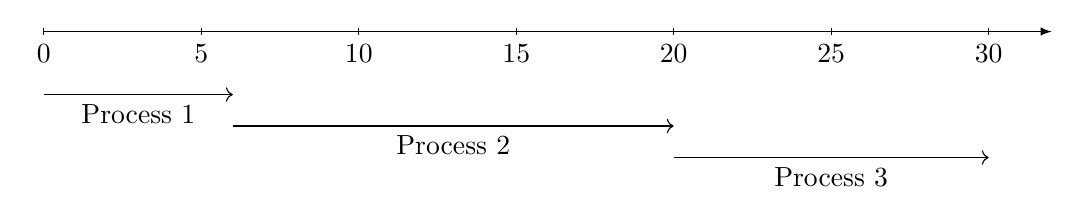
\begin{tikzpicture}[scale=0.4]
		\def\myNotes{1 / 0 / 6, 2 / 6 / 14, 3 / 20 / 10}
		\draw[-latex] (0, 0) -- (32,0);
		\foreach \x in {0, 5, 10, 15, 20, 25, 30}
		\draw[shift={(\x,0)},color=black] (0pt,3pt) -- (0pt,-3pt);
		\foreach \x in {0, 5, 10, 15, 20, 25, 30}
		\draw[shift={(\x,0)},color=black] (0pt,0pt) -- (0pt,-3pt) node[below] {$\x$};
		\foreach \pid/\start/\length [count=\i] in \myNotes
		\draw[->] ($ (\start, -1) - (0, \i) $) -- node[midway, below] {Process \(\pid\)} ++(\length, 0);
	\end{tikzpicture}
\end{highlight}

\paragraph{Wait Times}\label{par:wait_times}

For calculating the start time of a process we can use the general formula:
\[
	\text{wait time} = \text{start time} - \text{arrival time at CPU}
\]
Here are some examples using the data from our examples:
\begin{highlight}{First come first served CPU policy: wait times}
	\begin{align*}
		\text{Process \(1\)} & = 0 - 0 = 0   \\
		\text{Process \(2\)} & = 6 - 4 = 2   \\
		\text{Process \(3\)} & = 20 - 5 = 15
	\end{align*}
\end{highlight}

\paragraph{Average Wait Time}\label{par:average_wait_time}

The average wait time can be calculated by summing and dividing the wait times:
\begin{highlight}{First come first served CPU policy: average wait time}
	\begin{align*}
		\Sigma t     & = 0 + 2 + 15         \\
		\Sigma t     & = 17                 \\
		\overline{t} & = \frac{\Sigma t}{n} \\
		\overline{t} & = \frac{17}{3}       \\
		\overline{t} & = 3
	\end{align*}
\end{highlight}

\paragraph{Turnaround Time}\label{par:turnaround_time}

The turnaround time of a process can be calculated using the general formula:
\[
	\text{turnaround time} = \text{completion time} - \text{arrival time}
\]
Here are some examples using the data from our examples:
\begin{highlight}{First come first served CPU policy: turnaround time}
	\begin{align*}
		\text{Process \(1\)} & = 6 - 0 = 6   \\
		\text{Process \(2\)} & = 20 - 4 = 16 \\
		\text{Process \(3\)} & = 30 - 5 = 25
	\end{align*}
\end{highlight}

\subsection{Shortest job first}\label{sub:shortest_job_first}

Shortest job first is a simple to implement, non-preemptive scheduler that processes jobs in order of how much CPU time they still need.
SJF has the provable minimum average wait time, but many short jobs one after each other will increase the time a long job has to wait.

\paragraph{Time Diagram}\label{par:time_diagram_2}

\begin{highlight}{Shortest job first: time diagram}
	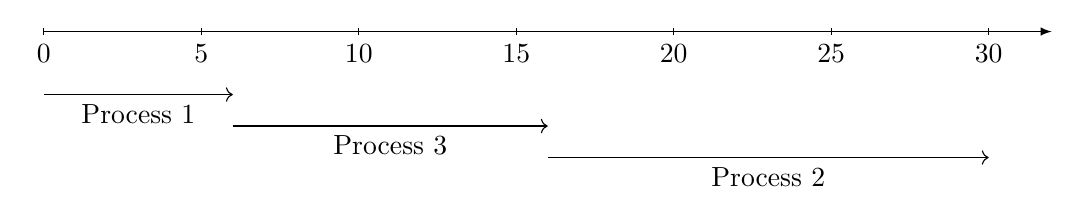
\begin{tikzpicture}[scale=0.4]
		\def\myNotes{1 / 0 / 6, 3 / 6 / 10, 2 / 16 / 14}
		\draw[-latex] (0, 0) -- (32,0);
		\foreach \x in {0, 5, 10, 15, 20, 25, 30}
		\draw[shift={(\x,0)},color=black] (0pt,3pt) -- (0pt,-3pt);
		\foreach \x in {0, 5, 10, 15, 20, 25, 30}
		\draw[shift={(\x,0)},color=black] (0pt,0pt) -- (0pt,-3pt) node[below] {$\x$};
		\foreach \pid/\start/\length [count=\i] in \myNotes
		\draw[->] ($ (\start, -1) - (0, \i) $) -- node[midway, below] {Process \(\pid\)} ++(\length, 0);
	\end{tikzpicture}
\end{highlight}

\paragraph{Wait Times}\label{par:wait_times_1}

For calculating the start time of a process we can use the general formula:
\[
	\text{wait time} = \text{start time} - \text{arrival time at CPU}
\]
Here are some examples using the data from our examples:
\begin{highlight}{Shortest job first: wait times}
	\begin{align*}
		\text{Process \(1\)} & = 0 - 0 = 0   \\
		\text{Process \(2\)} & = 16 - 4 = 12 \\
		\text{Process \(3\)} & = 6 - 5 = 1
	\end{align*}
\end{highlight}

\paragraph{Average Wait Time}\label{par:average_wait_time_1}

The average wait time can be calculated by summing and dividing the wait times:
\begin{highlight}{Shortest job first: average wait times}
	\begin{align*}
		\Sigma t     & = 0 + 12 + 1         \\
		\Sigma t     & = 13                 \\
		\overline{t} & = \frac{\Sigma t}{n} \\
		\overline{t} & = \frac{13}{3}       \\
		\overline{t} & = 4.3
	\end{align*}
\end{highlight}

\paragraph{Turnaround Time}\label{par:turnaround_time_1}

The turnaround time of a process can be calculated using the general formula:
\[
	\text{turnaround time} = \text{completion time} - \text{arrival time}
\]
Here are some examples using the data from our examples:
\begin{highlight}{Shortest job first: turnaround times}
	\begin{align*}
		\text{Process \(1\)} & = 6 - 0 = 6   \\
		\text{Process \(2\)} & = 30 - 4 = 26 \\
		\text{Process \(3\)} & = 16 - 5 = 11
	\end{align*}
\end{highlight}

\subsection{Shortest Time Remaining First}\label{sub:shortest_time_remaining_first}

This is effectively a preemptive version of Shortest Job First scheduling which also has a provably minimum average wait time.
Processes are added to the queue in order of the total time they still need to execute.
Where two processes need the same time, a First Come First Serve approach will be used.
Where a new processes has less time remaining than the current one, it gets priority.

\begin{note}
	The time diagram and calculations have been omitted here for brevity since they are \emph{exactly} as for Shortest Job First.
\end{note}

\subsection{Non-Preemptive Priority Scheduling}\label{sub:non_preemptive_priority_scheduling}

Non-Preemptive Priority Scheduling is an easy to implement scheduling system where each process is given a priority (a larger priority value means a lower actual priority) which is used to handle processes in order.
Where more than one process has the same priority as another, a First Come First Serve approach will be used.
This system can lead to lower priorities blocking indefinitely (``starvation'')

\begin{note}
	The time diagram and calculations have been omitted here for brevity since they are \emph{exactly} as for Shortest Job First.
	The reason they are the same an not instead executed in order \(3\), \(1\), \(2\) is: when the CPU starts, Process \(3\) is not available yet, so Process \(1\) is started.
\end{note}

\subsection{Round robin}\label{sub:round_robin}

The Round Robin system a preemptive version of the First Come First Serve system where processes are added to the queue in order of arrival.
The difference lies in that, if a process takes longer than a specified time quantum/time slice, they are suspended and moved to the end of the queue

Round Robin is also easy to implement, but here there may be very long wait times since each process will need to repeatedly wait for its time slice to come back -- performance depends heavily on the time slice value (think of extreme numbers).
We also see a slight performance hit since processes have to switch far more often.

\paragraph{Time Diagram}\label{par:time_diagram_3}

\begin{highlight}{Round robin: time diagram}
	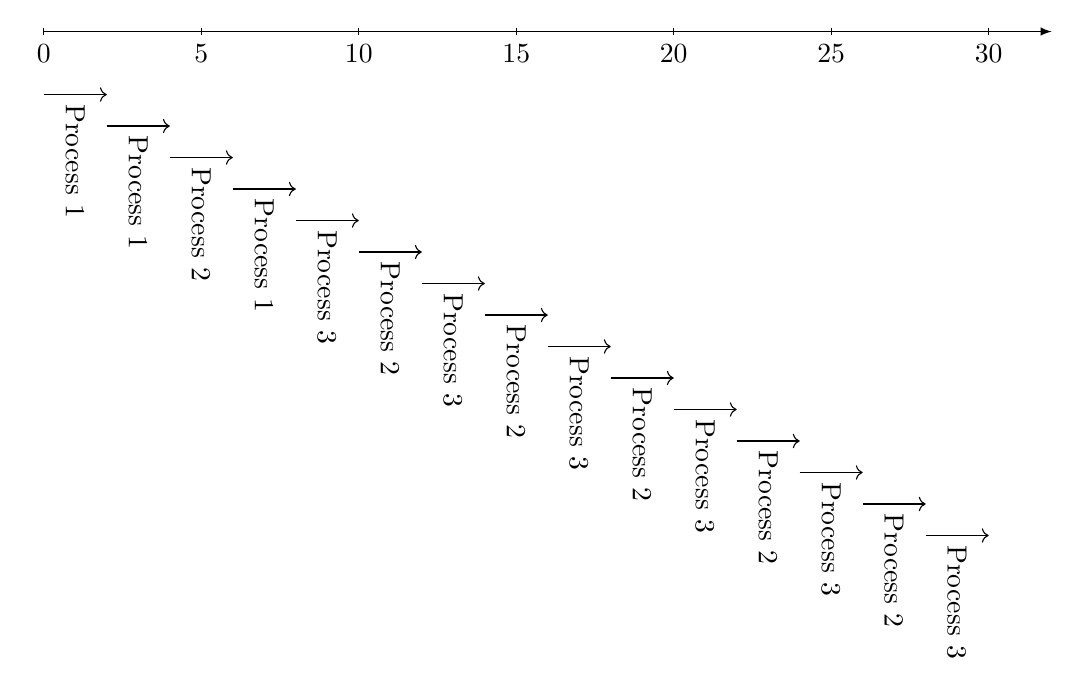
\begin{tikzpicture}[scale=0.4]
		\def\myNotes{1/0/2, 1/2/2, 2/4/2, 1/6/2, 3/8/2, 2/10/2, 3/12/2, 2/14/2, 3/16/2, 2/18/2, 3/20/2, 2/22/2, 3/24/2, 2/26/2, 3/28/2}
		\draw[-latex] (0, 0) -- (32,0);
		\foreach \x in {0, 5, 10, 15, 20, 25, 30}
		\draw[shift={(\x,0)},color=black] (0pt,3pt) -- (0pt,-3pt);
		\foreach \x in {0, 5, 10, 15, 20, 25, 30}
		\draw[shift={(\x,0)},color=black] (0pt,0pt) -- (0pt,-3pt) node[below] {$\x$};
		\foreach \pid/\start/\length [count=\i] in \myNotes
		\draw[->] ($ (\start, -1) - (0, \i) $) -- node[midway, right, rotate=-90] {Process \(\pid\)} ++(\length, 0);
	\end{tikzpicture}
\end{highlight}

\paragraph{Wait Times}\label{par:wait_times_2}

For calculating the wait time with Round Robin, just count the time between when the process was received by the processor and when it finishes executing where that process is not being handled.
\begin{highlight}{Round robin: wait times}
	\begin{align*}
		\text{Process \(1\)} & = 2  \\
		\text{Process \(2\)} & = 12 \\
		\text{Process \(3\)} & = 11
	\end{align*}
\end{highlight}

\paragraph{Average Wait Time}\label{par:average_wait_time_2}

The average wait time can be calculated by summing and dividing the wait times:

\begin{highlight}{Round robin: average wait times}
	\begin{align*}
		\Sigma t     & = 2 + 12 + 11        \\
		\Sigma t     & = 25                 \\
		\overline{t} & = \frac{\Sigma t}{n} \\
		\overline{t} & = \frac{25}{3}       \\
		\overline{t} & = 8.3
	\end{align*}
\end{highlight}

\paragraph{Turnaround Time}\label{par:turnaround_time_2}

The turnaround time of a process can be calculated using the general formula:
\[
	\text{turnaround time} = \text{completion time} - \text{arrival time}
\]
Here are some examples using the data from our examples:
\begin{highlight}{Round robin: turnaround times}
	\begin{align*}
		\text{Process \(1\)} & = 8 - 0 = 8   \\
		\text{Process \(2\)} & = 30 - 4 = 26 \\
		\text{Process \(3\)} & = 26 - 5 = 21
	\end{align*}
\end{highlight}

\section{Memory and Storage Management}\label{sec:memory_and_storage_management}

\subsection{Memory Management}\label{sub:memory_management}

Use the external storage (HDD, SSD) as ``add-on memory'' and keep only a \emph{subset} of the data of each process in the main memory and the rest on external storage.
Then, swap data in and out of memory to give each process the illusion that it has the entire system memory to work with.
Each process has its own \emph{virtual memory}.

The concept of a logical address space and a physical address space is central to proper memory management.
\begin{description}
	\item[Logical address] Also called a virtual address.
	      This is generated by the CPU and is where the process thinks the data is.
	\item[Physical address] This is where the data actually is.
	      The requests to the logical address are translated to physical addresses by the CPU.
\end{description}
When we transfer data between virtual and physical memory, we transfer fixed sized partitions called \emph{pages} instead of just words in order to save time.

\subsection{Storage Management}\label{sub:storage_management}

Here we are managing external storage to allow us to have data persistence.
The OS allows us to create, edit, delete files and directories (also backing up files and mapping files and permissions).

\subsubsection{OS and File Permissions}\label{ssub:os_and_file_permissions}

There are system calls to create files, delete files, move files, rename files, \dots.
\begin{itemize}
	\item When we \mintinline{python}{open(f)} files we search the directory structure on disk for \(f\) and move the contents to memory.
	\item When we \mintinline{python}{close(f)} we move the content of \(f\) in memory back to the disk again.
\end{itemize}

\subsection{File Protection}\label{sub:file_protection}

File owner/creator should be able to control what can be done by whom.
Types of access: read, write, execute, append, delete.

\section{More on OS Services}\label{sec:more_on_os_services}

\subsection{System Calls}\label{sub:system_calls}

\emph{System Calls} are programming interfaces to the services provided by the operating system.
We generally use a library that is build upon the direct system calls instead of using them directly.
A system call changes the processor from running in \emph{user mode} into \emph{kernel mode} where the operating system controls data on the CPU directly.
The CPU can do very low level operations with data directly on the CPU.

\subsection{Communication}\label{sub:communication}

We can use \emph{Inter-process Communication (IPC)} to allow processes to be either independent of cooperative.
Cooperative processes can be affected by other processes including sharing data.
There are some advantages to cooperative processes:
\begin{itemize}
	\item Information sharing
	\item Computation speedup (you don't need to write to external storage to transfer data)
	\item Modularity (can break down a large process)
	\item Convenience
\end{itemize}

\begin{note}
	Processors do much more:
	\begin{itemize}
		\item Multi-user services
		\item Real-time Operating Systems
		\item Managing multi-processor systems
		\item Managing distributed storage
		\item Virtualisation and hypervisors.
	\end{itemize}
\end{note}

\section{Introduction to Networks}\label{sec:introduction_to_networks}

\subsection{Why learn about computer networks?}\label{sub:why_learn_about_computer_networks_}

\begin{itemize}
	\item   How are systems connected together to form a network?
	\item How are networks connected?
	\item How does data go through the network to its destinations?
	\item How can we have reliable communications through unreliable links?
	\item What are the repercussions for programs that communicate over this infrastructure?
\end{itemize}

\subsection{Roles with Respect to Network Systems}\label{sub:roles_with_respect_to_network_systems}

\begin{description}
	\item[Users] The people that use a network don't have to worry about intricacies.
	\item[Manager] Manage a network
	\item[Application Designers] This is probably us. We have to worry about some details.
	\item[Designers of Systems] Have to have a deep knowledge of networks.
\end{description}

\section{Networked Systems}\label{sec:networked_systems}

Autonomous computing devices that exchange data to perform a goal.The exchange of data is visible to the application.
However, a computer system is only aware of the network (this is similar to how a computer writes to an IO device).

There is no single computer (or set of computers) that needs to organise data over a network (\emph{autonomous}).
Traffic on roads manages itself, but follows set rules.

\subsection{Key Aspects}\label{sub:key_aspects}

\begin{description}
	\item[Communication] How is information exchanged across a single link?
	\item[Networking] How are links interconnected to build a network?
	\item[Networked Systems] How do systems communicate across the network?
\end{description}

\subsection{Applications Using Networks}\label{sub:applications_using_networks}

Some applications use The Internet World Wide Web:
\begin{itemize}
	\item Email
	\item Social Networks
	\item Streaming audio and video
	\item File sharing
	\item Instant messaging
\end{itemize}
Others don't:
\begin{itemize}
	\item Digital TV
	\item Mobile voice telephony
	\item Sensor networks
	\item Controller area networks connecting sensor and other components inside vehicles or aircraft (eg. on board computers in car)
\end{itemize}

\subsection{Communication}\label{sub:communication_}

Messages are transferred from source to destination via a communication channel.
The size of messages might be bounded.

\paragraph{Information Required For Communications}\label{par:information_required_for_communications}

\begin{itemize}
	\item Communication might be \emph{simplex} (one way), \emph{half-duplex} (both ways, one at a time), \emph{full-duplex} (both ways all of the time).
	\item We want to communicate data; messages convey information.
	\item How much information is in a message? We can calculate this mathematically (not covered here).
	\item What is the information carrying capacity of a channel?
	\item Capacity of channels to convey information can be modelled using how much power they use, how much they can transfer and how quickly they can do it.
	\item Physical limits exist on the capacity of a channel.
\end{itemize}

\subsubsection{Physical Forms of Messages}\label{ssub:physical_forms_of_messages}

A physical form of a message can be a material object (carrier pigeon, CD, etc.), but is usually a wave (sound, electrical, etc.) and may be analogue or digital.

\paragraph{Analogue Signals}\label{par:analogue_signals}

The simplest analogue signal means that amplitude directly codes the value of interest: louder voice means louder signal, AM radio, analogue telephones.

These can be arbitrarily accurate, but are susceptible to noise and interference and are difficult to process with digital electronics.

\paragraph{Digital Signals}\label{par:digital_signals}

These comprise a sequence of symbols and not arbitrary values (the underlying channel can still be analogue though and modulation will be used to convert the signal).

Computer systems use binary encoding much like networked systems too.

\begin{description}
	\item[Bit Rate] The bits per second
	\item[Baud Rate] The symbols per second (one symbol is not one bit).
\end{description}

\paragraph{Analogue to Digital Conversion}\label{par:analogue_to_digital_conversion}

\begin{enumerate}
	\item Sample the signal at a suitable rate (higher is better).
	\item Quantise each value to the nearest allowable discrete value.
	\item Convert to a digital representation.
\end{enumerate}
The \emph{sampling theorem} determines that rate at which the signal must be sampled for accurate reconstruction.

\section{Channels, Links, Networks and Switching}\label{sec:channels_links_networks_and_switching}

\begin{description}
	\item[Hosts] The source and destination for messages
	\item[Signal] A signal is conveyed via a channel and may be directly conveyed on a cable, or it may be modulated onto an underlying carrier.
	      There will probably be many links that the channel has to go through.
	\item[Link] A link directly connects one or more nodes together.
	\item[Network] A network comprises several links connected together.
	      The devices connecting the links are called their switches or routers.
\end{description}

\subsection{Network Switching}\label{sub:network_switching}

Network switching describes how devices can share a single wire to communicate.

\subsubsection{Circuit Switched Networks}\label{ssub:circuit_switched_networks}

A dedicated circuit can be set-up between two points.
There the two devices can exchange arbitrary length messages.
There is a guaranteed capacity once the network is created, but the dedicated circuit can block other communications from other devices.

\subsubsection{Packet Switched Networks}\label{ssub:packet_switched_networks}

Messages are split into small packets (small, size constrained chunks) before transmission.
Allows more than one pair of devices to communicate.
Connectivity is guaranteed, but the average capacity varies depending on how many people are using the network.

\section{Protocols and Layers}\label{sec:protocols_and_layers}

\subsection{Network Architecture}\label{sub:network_architecture}

A network architecture is organised into layers in order to manage the complexity of network communications (encoding conversion, route to take, fiber network conversions, \dots).

\subsection{Layers}\label{sub:layers}

\begin{enumerate}
	\item Application programs
	\item Process-to-process channels (IRC to IRC)
	\item Host-to-host connectivity
	\item Hardware (what happens in the wires?)
\end{enumerate}

\subsection{Network Protocols}\label{sub:network_protocols}

Each layer in the network architecture will have its own protocol.
To be useful, the messages need to follow a set syntax and have agreed semantics.
Protocols have an agreed language for encoding message and rules for what messages mean and when they can be sent.
Protocols define the behaviour of the network too through the interactions of devices.

\subsubsection{Interfaces}\label{ssub:interfaces}

Each protocol object (an implemented protocol) has two interfaces:
\begin{description}
	\item[Service Interface] Performs the actual operations on this protocol.
	\item[Peer-to-peer Interface] Messages that are exchanged with the peer.
	      This is how services are requested.
	      The service interface sends messages through this.
\end{description}

\subsubsection{Protocol Data Units}\label{ssub:protocol_data_units}

A PDU defines what messages are legal to send.

\paragraph{Syntax}\label{par:syntax}

A protocol will have different types of message called Protocol Data Units (PDUs).
Each type of PDU will have a syntax, etc., that describes what information is included and whether it is textual data or binary data.

\begin{description}
	\item[Textual PDUs] These have a syntax and grammar that describes their format (similar to how programming languages have a grammar).
	\item[Numeric PDUs] These have rules too like is the data big or little endian? \(32\) or \(64\) bit? Fixed or variable length?
\end{description}

\paragraph{Semantics}\label{par:semantics}

Protocol semantics defined when PDUs can be sent and what response is needed.
\begin{itemize}
	\item Who can send PDUs
	\item Roles for hosts (client and server, peer-to-peer)
	\item What are entities and how are they named?
	\item How are errors handled?
\end{itemize}
A state transition diagram can be used to indicate the stages of a protocol operation and the transitions that occur in response from PDUs with what can be sent back.

\section{Protocol Layering}\label{sec:protocol_layering}

Communication systems are a series of layers to manage complexity, modularity, separation of concerns.
Each layer offers services to the higher layers using services from lower  layers.
The highest layer is the applications that we use, the lowest layer is the physical connections.

Peers at some layer \(i\) communication via the layer \(i\) protocol using lower layer services.

\subsection{OSI Reference Model}\label{sub:osi_reference_model}

The OSI Reference Model is a way of thinking about layered protocol design.
It is a design tool, since realistic implementations will be far more complex and more closely related to the \emph{TCP/IP (or the Internet)} model.

\begin{note}
	All nodes implement the bottom three layers (network, data link, physical) because they all need this information.
\end{note}
\subsection{Physical Layer}\label{sub:physical_layer}

Handles the transmission of raw bits over a communication link.
Defines attributes of the physical medium of communication:
\begin{itemize}
	\item Size and shape of plug
	\item Type of wire
	\item Radio frequency
	\item Modulation scheme
	\item Transmission power
	\item Electrical voltage
\end{itemize}

\subsection{Data Link Layer}\label{sub:data_link_layer}

The structure and frame of the physical layer bit stream.
This layer splits the bits in to individual \emph{frames}.
\begin{itemize}
	\item Detect and correct errors in messages using parity and ECC or acknowledgements.
	\item Access Control
	      \begin{itemize}
		      \item Assign addresses to each host on the link (MAC or IP address)
		      \item Allow access to link and allow hosts to send messages
		      \item Rate limit to ensure all hosts get fair access and avoid overwhelming hosts.
	      \end{itemize}
\end{itemize}

\subsection{Network Layer}\label{sub:network_layer}

Connects several links to form a connection between a source and a destination.
\textbf{Handles routing among nodes within a packet switched network.}

\begin{note}
	The unit of data exchanged between nodes in this layer is called a \emph{packet}.
\end{note}
\begin{note}
	Because these networks can be worldwide, the layer must be standardised (even more so than at any of the other layers).
\end{note}

\subsection{Transport Layer}\label{sub:transport_layer}

This layer handles the end-to-end transfer of data from the source process to the destination process (a \emph{process-to-process channel}).
The unit of data here is called a \emph{message}.
A transport layer provides:
\begin{itemize}
	\item Reliability
	\item Ordering
	\item Framing
	\item Congestion control
\end{itemize}
But the availability of each of these depends on the guarantees made in the network layer.

\subsection{Session and Presentation Layers}\label{sub:session_and_presentation_layers}

\subsubsection{Session Layer}\label{ssub:session_layer}

The session layer provides a place (namespace) to bunch several different transport streams together in one application.
eg., audio and video streams happening at the same time.

\subsubsection{Presentation Layer}\label{ssub:presentation_layer}

Manages the presentation, representation and conversion of data (character set, markup languages, data format conversion).

\subsection{Application Layer}\label{sub:application_layer}

Here we are talking about user application protocols (HTTP) and not the application themselves (Firefox):
\begin{itemize}
	\item HTTP
	\item FTP
	\item SSH
	\item \dots
\end{itemize}

\subsection{Protocol Standards}\label{sub:protocol_standards}

A standard is a formal definition of a network protocol to ensure interoperability.
Standards can be openly defined or closed source, restricted or free, collaborative or combative, etc.

Not all players in the standard process have the same goals:
\begin{itemize}
	\item Delaying a standard to allow a different solution to get market share
	\item Including intellectual property, patented technologies to get royalties, etc.
	\item Enhancing (or subverting) the security of a protocol.
\end{itemize}
Standards are required, but they may not always be the best solution.

\section{Physical and Data Link Layers}\label{sec:physical_and_data_link_layers}

These are the layers that interact with the physical hardware.
The physical layer defined what will happen in the hardware.
The data link layer still has to worry about the physical connections so that it can handle the data connection properly.

\begin{note}
	These layers usually differ from device to device.
\end{note}

\subsection{Physical Layer (or \(L1\))}\label{sub:physical_layer_or_mkl1_}

The physical layer is the only layer that when it speaks to its peer is actually physically connected to it.

The main focuses are to transmit a sequence of bits over an analogue channel subject to noise/hardware limitations/clock skew (time sensitive events are late), and interface to \(L2\).

\subsubsection{Examples}\label{ssub:examples}

\paragraph{Unshielded Twisted Pair}\label{par:unshielded_twisted_pair}

An electrical cable with two wires twisted together.
Each pair is one direction of signal and ground.
\begin{itemize}
	\item Twists reduce interference and noise pickup
	\item Can be hundreds of metres long and still work well
	\item Longer cables are more noisy
	\item Used in Ethernet and telephones.
\end{itemize}

\paragraph{Optical Fibre}\label{par:optical_fibre}

Glass core with shielding.
Fragile and can only transmit in one direction.
Low noise, high capacity, low cost, but requires expensive lasers to operate.

\subsubsection{Encoding Data For Wired Data Transmission}\label{ssub:encoding_data_for_wired_data_transmission}

Signal will be transported as binary.
The signal is usually put straight onto the channel without any conversion at all (unlike for a wireless data connection).
Encoding is done by changing the brightness or voltage.

\paragraph{Baseband Data Encoding}\label{par:baseband_data_encoding}

The signal is in its original frequency range (it has not been modulated to a higher frequency).
We encode the signal as a change in voltage or brightness.

If there are too many \(1\)s or \(0\)s in a row, it can be hard to tell exactly how many signals arrived.
To solve this, we can encode a \(1\) as a change in signal and a \(0\) as no change (NRZ inverted) instead of having the data encoded directly (NRZ).
This still has a problem for long lengths of \(0\)s though since the signal doesn't change.

\emph{Manchester encoding} solves this completely where a low-high transmission is encoded as \(0\) and a high-low transmission is encoded as \(1\).
Manchester increases the bandwidth requirement because the frequency is now double.

\subsubsection{Carrier Modulation}\label{ssub:carrier_modulation}

The baseband is the range of frequencies I want to transmit (the original data before modulation).
When we modulate, we convert the baseband data to become a higher frequency based on the data itself.

This allow you to have several signals on the same channel by having data on the same baseband frequency modulated to a free frequency for each signal.
Generally this is used for wireless links, but can be used for wired links too (ADSL and voice telephones use same wires).

\section{Bandwidth}\label{sec:bandwidth}

The bandwidth of a channel defines the frequency range it can transport (based on the physical limitations of the hardware itself).
The maximum transmission rate of a digital signal depends on the channel bandwidth:

\smallskip
\begin{minipage}{0.4\linewidth}
	\centering
	\scalebox{2}{
		\begin{math}
			R_{max} = 2H\log_2 V
		\end{math}
	}
\end{minipage}
\hfill
\begin{minipage}{0.55\linewidth}
	Where:
	\begin{itemize}
		\item \( R_{max} \) = maximum transmission rate of channel (bits per second)
		\item \(H\) = Bandwidth \(Hz\)
		\item \(V\) = number of possible discrete values per symbol (the size of the alphabet used).
	\end{itemize}
\end{minipage}
\begin{note}
	We assume a noise free channel here.
\end{note}

\subsubsection{What is \(V\)}\label{ssub:what_is_mk}

\(V\) is the possible discrete values per symbol (size of the alphabit).
Inside a computer system, we use binary (or \(V=2\)).
In a physical communication channel, we can have a larger alphabet so that each symbol has more data.

\subsection{Channel Capacity and Noise}\label{sub:channel_capacity_and_noise}

Real world channels have noise that alters the signal.
We can measure a channel's signal power, \(S\), and noise floor, \(N\), and compute the signal to noise ration (\(SN\) or \(SNR\)).

Bandwidth and \(SNR\) are fundamental limits on the throughput (bit rate) which might be able to be reached using careful engineering, but can never be surpassed (Shannon's Theorem).






\section{Data Link Layer (L2)}\label{sec:data_link_layer_mkL2}

This layer and the \emph{Physical Layer} are both dependent on the physical medium of the channel and are called \emph{Media Layers}.

\subsection{Purpose of the Data Link Layer (DLL)}\label{sub:purpose_of_the_data_link_layer_dll_}

The Data Link Layer handles the physical connection for devices directly connected via a link.
\begin{description}
	\item[Addressing] Identifies devices
	\item[Frame] Structure the raw bit stream into a usable format
	\item[Error Correction] Correct errors in the code from noise or interference
	\item[Access Control] Also ``media access control''.
	      Decides which devices can communicate on a channel.
\end{description}
The data link layer communicates with \(L_1\) via a raw bit stream and it provides \(L_3\) with structured communication (using addressing and packets).

\subsection{Addressing}\label{sub:addressing}

Physical links can be direct between two devices, but several devices can be connected to several others too (like in a wireless link).
Multi-access links need host addresses so we can identify senders and receivers (for a direct connection, there is only one route).

An address may be \emph{link-local} or \emph{global scope}.
It is sufficient for addresses to be unique among the devices which are actually attached to each other, but there needs to be communication between devices to create addresses.
To avoid this negotiation (and make switching networks simpler, and also avoid privacy concerns), most data link layer protocols use a globally unique address (ethernet, wifi).

\begin{note}
	The addresses here are assigned to the network interface itself and not the node system.
\end{note}

\subsection{Framing and Synchronisation}\label{sub:framing_and_synchronisation}

The physical layer provides an unreliable raw bit stream in a long stream on unstructured bits that may be corrupted or timing could be disrupted.

The data link layer corrects these problems by breaking the stream into individual frames which are then transmitted and corrected to limit the damage of any errors transmitted.
For example, if there is an error, only one frame has to be resent.

\subsubsection{Frame Synchronisation}\label{ssub:frame_synchronisation}

We need the transmitter and receiver to agree on where the start and end of messages are to work properly.
We can either:
\begin{itemize}
	\item Leave a gap in between the frames.
	      This is difficult because setting a uniform time gap needs agreement on clock time and delay time.
	\item Have a length field.
	      This doesn't work very well either because the length can become corrupted too.
	\item A special code to signal the beginning of a frame.
	      The unique bit pattern only happens at the start of a message.
	      If there is an error somewhere in the message, we can just wait for the next header signal.
	      What if this code is somewhere in the data? \emph{Bit stuffing.}
\end{itemize}

\subsubsection{Bit Stuffing}\label{ssub:bit_stuffing}

If the code was a sequence of \(6\) consecutive \(1\)s, and these \(6\) \(1\)s appear somewhere in the data, an extra \(0\) will be ``stuffed'' in between the \(5\)th and \(6\)the bits.

The header is wrapped in \(0\)s on either side, so if a sequence of \(7\) \(1\)s appears, the receiver will know that this is a corrupt frame.

\subsection{Error Detection and Correction}\label{sub:error_detection_and_correction}

Noise and interference at the physical later can cause bit errors.
This is generally rare in wired links, and more common in wireless systems.
We add error detection code to each packet to solve this.

We add some redundant data that is calculated using the data being sent (like a hash).
When the packet arrives, the receiver tries to calculate the error correction code again and checks it still matches what was sent as the code.

\subsubsection{Parity Code}\label{ssub:parity_code}

This is the simplest error detecting code.
\begin{itemize}
	\item If there is an odd number of \(1\)s in the data, the parity bit is a \(1\).
	\item If there is an even number of \(1\)s in the data, the parity bit is a \(0\).
\end{itemize}
Either way there will be an even number of bits total (data and parity), so if you get an odd number, there has been an error.
The parity is the XOR of the data bits.

\begin{note}
	This method only detects when an odd number of bits are incorrect so this is only useful really for a small selections of data.
\end{note}

\subsubsection{Internet Checksum}\label{ssub:internet_checksum}

Here, we add up all of the data values (\(16\) bits one's complement here)
The receiver recalculates the checksum, if there is a mismatch, there has been an error.
This method is more effective than parity codes because it can detect most multiple bit errors.

\begin{note}
	For one's complement, if there is a carry out at the end, we just re-add it.
\end{note}

\begin{note}
	There are even more powerful error detecting codes like \emph{Cyclic redundancy code} (CRC) which is more complex and leads to fewer undetected errors.
\end{note}

\subsubsection{Correcting Errors}\label{ssub:correcting_errors}

We can also transmit error correcting code as additional data with each frame.
A simple method of doing this is to just transmit the data twice, but \emph{Hamming code} is a smaller way that can correct a single bit, and sometimes more than one.

Other error correcting codes exist, but there is a trade-off between complexity, the amount of data added and the ability to correct multi-bit errors.

\begin{note}
	If the data is completely unsalvagable, we can just request retransmission.
\end{note}

\subsection{Media Access Control}\label{sub:media_access_control}

Links may be point-to-point or multi-access.
\begin{description}
	\item[Point-to-point] There are separate physical cables for each direction.
	      We need framing in each direction, but there is no competition (contention) for the links.
	\item[Multi-access] There is a single bidirectional link for all hosts so nodes have to compete (contend) for access.
\end{description}

\subsubsection{Contention}\label{ssub:contention}

When two hosts transmit simultaneously, there will be a collision.
If the signals were to overlap, only garbage would be received.

\subsection{Contention-Based MAC}\label{sub:contention_based_mac}

We need a two stage access to a channel.
\begin{enumerate}
	\item Detect if a collision is happening, or will happen by listening to the channel before and while sending.
	\item Send if there is no collision, or wait and retransmit later (the delay is randomised and increasing to avoid repeated collisions. eg., two people accidentally interrupting each other).
	      Many collisions means the network is congested and needs time to recover.
	      This delay can be arranged to give certain hosts, users, or traffic priority.
\end{enumerate}

\begin{note}
	This system is entirely distributed without any central  system to decide when to transmit.
\end{note}
\noindent
Access to the channel is:
\begin{itemize}
	\item Probabilistic (not deterministic)
	\item Of variable latency
\end{itemize}

\subsubsection{ALOHA Network}\label{ssub:aloha_network}

This is a wireless network developed at the University of Hawaii in \(1970\).

The system was to simple transmit whenever data was available (no attempts to preempt collisions)
When a collision happened (while transmitting), just wait a random time and retransmit.

This is a very simple system, but has poor performance and results in low channel utilisation (which means long delays).

\subsubsection{Carrier Sense Multiple Access}\label{ssub:carrier_sense_multiple_access}

Here when the propagation delay is low, we listen before sending.
\begin{itemize}
	\item If there is another transmission active: back off as if a collision has actually occurred.
	\item If the link is idle, send data immediately.
\end{itemize}
This system improves link utilisation by avoiding interrupting active transmissions (only the new sender backs off if the channel is active).

If you have a high propagation delay, you should listen before and while you are sending data.
If a collision occurs, stop sending data immediately, back of and retransmit.
\begin{note}
	Both packets are still corrupted, but the time the channel is blocked is far less giving better performance.
\end{note}

\paragraph{Why does propagation delay matter?}\label{par:why_does_propagation_delay_matter_}

If you are listening to a channel and there is silence, on a low delay network, you can be confident no nodes are transmitting.
If there is a high delay, though, another node may be transmitting and the signal hasn't reached you yet and causing a collision and garbling data.



\section{Introduction to the Network Layer (L3)}\label{sec:introduction_to_the_network_layer}

The network layer addresses the problem of building networks of networks.
Previously, we have had point-to-point and multiple-access networks with hubs and switches to create a local network.

The Network Layer is the first end to end layer in the OSI layer meaning it is responsible for the end to end delivery of data across many link-layer hops and autonomous systems.
We can create an inter-network network (or internet).

\subsection{Components}\label{sub:components_}

\subsubsection{Common end-to-end network protocol}\label{ssub:common_end_to_end_network_protocol}

A common end-to-end protocol provides a single seamless service to interface with the transport layer above it by delivering data packets (or by provisioning circuits in a circuit switched network) and addressing each end system.

\subsubsection{Routing Devices}\label{ssub:routing_devices}

A routing device will connect one network to another by implementing the common network protocol.
A gateway or router will hide differences in the link layers between the networks:
\begin{itemize}
	\item Framing
	\item Addressing
	\item Flow control
	\item Error detection and correction
\end{itemize}
with the least amount of effort possible.

\subsection{The Internet}\label{sub:the_internet}

\begin{description}
	\item[1965] Concept of packet switching
	\item[1969] Wide-area packet networks
	\item[1973] First non-US ARPANET sites
	\item[1974] Initial version of the internet protocol
	\item[1981] Access to ARPANET broadened to non-DARPA funded sites.
	\item[1983] Switched to IPv4
	\item[1992] Development of IPv6 starts
\end{description}

\section{The Internet Protocol}\label{sec:the_internet_protocol}

The internet protocol is a common abstraction layer to interface with the transport protocols above it and the data link (and physical) layers below it.
\begin{itemize}
	\item Simple
	\item Best effort
	\item Connectionless
	\item Packet delivery
\end{itemize}
Providing:
\begin{itemize}
	\item End-to-end global addressing
	\item Routing
	\item Fragmentation and reassembly (breaking up packets)
\end{itemize}
Key concepts:
% TODO: make subsections
\begin{itemize}
	\item Global inter-network protocol
	\item Hour glass protocol stack:
	      \begin{itemize}
		      \item Many transport and application layers
		      \item A single network layer protocol:
		            \begin{itemize}
			            \item Packet switched, best effort service
			            \item Uniform network and host addressing
			            \item Uniform end-to-end connectivity
			            \item Range of link-layer technologies
		            \end{itemize}
	      \end{itemize}
\end{itemize}

\subsubsection{Basic Routing and Delivery}\label{ssub:basic_routing_and_delivery}

The packets are just sent, there is no permanent connection.
There are no guarantees made so packets could be delayed, dropped, corrupted or duplicated.
Any packets that cannot be delivered are just discarded.

\subsection{The Internet Protocol Packet}\label{sub:the_internet_protocol_packet}

Every network interface on every host is intended to have unique address (these are internet protocol addresses or ``logical addresses'').

\begin{description}
	\item[IPv4] These are \(32\) bit addresses (\(130.209.241.197\)) which is made up of \(4\) sets of \(8\) bit decimal numbers.
		There are not very many addresses.
	\item[IPv6] These are \(128\) bit addresses which are \(4\) sets of \(4\) hexadecimal digits.
\end{description}

\subsection{Fragmentation}\label{sub:fragmentation}

The maximum frame size of the link layer is \(1500\) bytes so IPv4 routers will split up (fragment) packets which are larger than this (MTU size).
A special bit is set (MF) is set if more fragments are still to follow.

In IPv6 there is no support for fragmentation in transit so packets must be split up on the hosts themselves.

\subsection{Loop Protection}\label{sub:loop_protection}

Some packets could loop forever and just take up processing power so packets include a forwarding limit which is a value (usually \(64\) or \(128\)) that each router reduces by \(1\) until it is discarded at \(0\).

\subsection{Header Checksum}\label{sub:header_checksum}

IPv4 header contains a checksum to detect and corruption introduced during transmission.
This is quite similar to the link-layer checksum, but uses a different algorithm.
\begin{note}
	This exclusively protects the header -- the data should be protected in an upper layer protocol.
\end{note}
\noindent
IPv6 does not contain a checksum and assumes the header and data will be protected on the link later.

\subsection{Transport Layer Protocol Identifier}\label{sub:transport_layer_protocol_identifier}

Network layer packets include the transport layer data as a payload:
\begin{itemize}
	\item TCP (\(6\))
	\item UDP (\(17\))
	\item DCCP (\(13\))
	\item ICMP (\(1\))
\end{itemize}
These are managed by the IANA.

\subsection{Differentiated Services}\label{sub:differentiated_services}

End systems can request special services from the network.
\begin{itemize}
	\item Emergency traffic should have priority
	\item Gaming or telephony prefer low latency, but don't need high bandwidth
	\item Background software might ask for low priori
\end{itemize}
You can signal your preference using a \emph{differentiated service code point (DSCP)} field in the header.
These are only a hint and can often be stripped away at network boundaries.
There can be difficult issues like ``who is allowed to set the DSCP?'' and ``what are people charged for setting the DSCP''?

\subsection{IPv4 or IPv6}\label{sub:ipv4_or_ipv6}

IPv4 has reached its end of life since there are no addresses left.

IPv6 is supposed to be a long-term replacement for IPv4.
The primary goal is to increase the address size to allow more hosts on the network.
An additional benefit is that the protocol is simple which makes high speed implementations easier.

It is not yet clear if IPv6 will be widely deployed, but it is very easy to build applications that use both.
A DNS query will return a IPv6 address if possible.

\section{IP Addressing}\label{sec:ip_addressing}

There are a few challenges:
\begin{enumerate}
	\item Is the address an identify or a location? Does it name the host or the location where it is?
	\item How should addresses be allocated? Do we use a hierarchical system or just allocated them flat?
	\item What is the address format? A number or text? Human readable? Fixed or variable length?
\end{enumerate}

\subsection{Identity and Location}\label{sub:identity_and_locaiton}

An address can denote the identity of a host.
A host should have a consistent address, irrespective of where or when they attach to the network to simplify upper-layer protocols (transport layer and applications don't care if you move about since the IP address doesn't change).
Complexity is moved to the network layer.

The network layer must know the location of the destination host so it can send data to it.
Sometimes a database is used to attach an identity to its address.

Alternatively, an address can indicate the location which a host attaches to the network.
This simplifies the network layer since it can send data directly to a host, but makes the higher layers more complex since they have to handle the changing IP addresses.

\subsection{Address Allocation}\label{sub:address_allocation}

We can have a hierarchical system where there is a common prefix or suffix for a set of machines.
This requires a rigid control of allocations.

If we just use a flat allocation, we cannot filter by an are like we can with a hierarchical system, but allocations can happen much more flexibly.

\subsection{Address Format}\label{sub:address_format}

Fixed length binary is easier for machines to read, but variable length text is better for humans.

\subsection{IP Addresses}\label{sub:ip_addresses}

IP addresses:
\begin{itemize}
	\item Specify the location of a network interface
	\item Are allocated hierarchically
	\item Are of a fixed size (either \(32\) bits or \(128\) bits).
\end{itemize}
A host with several network interfaces will have an IP address for each interface (like for Wi-Fi and Ethernet).
Both IPv4 and IPv6 addresses are hierarchical, and encode location by splitting addresses into a host and a network.
\begin{description}
	\item[Netmast] Describes the number of bits in the network part as a mask (\(1\) is a network,  \(0\) is a host).
	\item[Network] The network itself has the address wit the host part equal to \(0\).
	\item[Broadcast] The broadcast address has the address with the host section all \(1\)s.
\end{description}

\subsubsection{IP Address Management}\label{ssub:ip_address_management}

\paragraph{IPv4}\label{par:ipv4}

IPv4 only has \(2^{32}=4,294,967,296\) addresses.
The IANA administers the pool of unallocated addresses.
Addresses assigned to Regional Internet Registries (RIRs) can then assign to ISPs and large enterprises within their region (ISPs can then allocate to their customers)

\paragraph{IPv6}\label{par:ipv6}

IPv6, if deployed, will solve our address shortage issue for a \emph{long} time.
There are \(2^{128}=340,282,366,920,9938,463,463,374,607,431,768,211,456\) total addresses.

\subsection{IPv6 Deployment Issues}\label{sub:ipv6_deployment_issues}

IPv6 requires changes to be made to every host, router, firewall and application.
So far, most backbone routers support IPv6 and well as most operating systems, but there is still lots to go.


\section{Routing}\label{sec:routing}

In a network, nodes learn only a subset of the network topology and runs an algorithm to decide where to forward packets destined for other hosts.

\begin{itemize}
    \item End hosts (consumer devices) usually only know what is and isn't on your local network and use only a simple algorithm.
          If a packet is for the outside network, packets are sent to the default gateway.
    \item Gateway devices (routers) exchange information to decide on the best route based on their knowledge of the network.
\end{itemize}

\subsection{Unicast Routing}\label{sub:unicast_routing}

We route to deliver packets from one source to one destination.
The choice of algorithm used can vary:
\begin{itemize}
    \item Intra-domain routing
    \item Inter-domain routing
    \item Politics and economics
\end{itemize}

\subsubsection{Inter-domain unicast routing}\label{ssub:inter_domain_unicast_routing}

Each network/internetwork is entirely autonomous and can have different policies and technologies.
These operate potentially with distrust.

\subsubsection{Intra-domain unicast routing}\label{ssub:intra_domain_unicast_routing}

Here we are routing inside of an autonomous system.
There is a single trust domain where there are no restrictions on which links can be used or who can determine the network topology.

With access to the whole network, you can make the best use of the network you have available to give the most efficient routing.

There are two approaches to routing packets in an intra domain system:
\begin{itemize}
    \item Link state
    \item Distance
\end{itemize}

\subsection{Inter-domain Routing}\label{sub:inter_domain_routing}

Here the goal is to find the best route to the destination network.
Each network is treated as a single node and routing is done ignoring the internal topology.

The network is made up of autonomous systems where each autonomous system is an independently administered network.

\begin{note}
    Some nodes can have several exit points (``not on the edge''), so there needs to be some logic here, or a ``routing table''.
\end{note}

\subsubsection{Edge Routing}\label{ssub:edge_routing}

Where you have multiple exits to a network, you have a \emph{default free zone} where there is no default exit point.
We must route based on policies and not the shortest route.
\begin{itemize}
    \item Use autonomous system \(x\) in preference to AS \(y\).
    \item Use AS \(x\) to reach only specific addresses
    \item Use the path that crosses the fewest ASes
    \item Avoid ASes located in a country.
\end{itemize}
All of these require a complete AS-level knowledge of the network.

We use a protocol named \emph{border gate way} protocol (BGP) which runs on specific routers to exchange data between ASes.
The individual ASes choose which internal routes to expose.
These are complex and policy driven.

\section{Intra-Domain Routing}\label{sec:intra_domain_routing}

Intra-domain routing works inside of a domain (any network or internetwork operated by a single entity: an autonomous system) and operates a single routing protocol which is typically the OSPF (open shortest path first) where you exchange routes to IP address prefixes (prefixes point to networks).

\subsection{Distance Vector Protocol}\label{sub:distance_vector_protocol}

Each node has a table containing the distance to each node in the network which is periodically exchanged with neighbours so eventually each node will know the distance to all other nodes (``converges'')

\begin{note}
    Nodes only update their own tables if there has been a change on another node.
\end{note}
At each node we store the following data for each node in the network:
\begin{itemize}
    \item Cost which is the length of the path to \(x\).
    \item The next hop which is the next node on the path to \(x\).
          A \(-\) signifies an unknown hop and a \(\cdot\) signifies that no hop is needed.
\end{itemize}

\paragraph{Time Step One}\label{par:time_step_one}

\begin{itemize}
    \item Nodes are initialised and only know their immediate neighbours.
    \item All nodes update their own local rows with their neighbours too.
\end{itemize}

\paragraph{Time Step Two}\label{par:time_step_two}

\begin{itemize}
    \item Routing data has spread by one hop so we can reach nodes two hops away (each node knows its neighbours).
    \item Nodes report their route tables to their neighbouring nodes, which are merged together to find the shortest routes.
    \item At the end of the second time step, we can reach nodes three stops away.
\end{itemize}

\paragraph{Time Step Three}\label{par:time_step_three}

\begin{itemize}
    \item (From the example) routing data has spread two hops and the routing tables are now complete.
\end{itemize}

\paragraph{Time Step Four}\label{par:time_step_four}

\begin{itemize}
    \item Nodes continue to exchange distance metrics in case the network topology changes.
\end{itemize}

\section{The Transport Layer (L4)}\label{sec:the_transport_layer_l4_}

The transport layer aims to hide network complexities and unreliableness, and enhance the overall quality of service (QoS) of the network layer to higher layers.
The transport layer provides:
\begin{itemize}
	\item An easy to understand service model
	\item An easy to use programming API
\end{itemize}
And offers these functions:
\begin{itemize}
	\item Addressing and multiplexing
	\item Reliability
	\item Framing
	\item Congestion control
\end{itemize}

\begin{note}
	Previously, layers have been communicating between hosts, here we are communicating between processes.
\end{note}

\subsection{Addressing and Multiplexing}\label{sub:addressing_and_multiplexing}

The network layer address identifies a host.
The transport layer address identifies a user process running on a host, so multiple services operating at the transport layer level are multiplexed in to a single IP-based layer.

\subsection{Reliability}\label{sub:reliability}

The network layer is unreliable (``best effort'') and even reliable network circuits may fail.
The transport layer makes the quality of service better to match application needs (``appropriate end to end reliability'' -- executable downloads need \(100\)\% accuracy, video playback doesn't).

\subsection{Framing}\label{sub:framing}

If an application wants to send structured data over a network, the transport layer will maintain the boundaries.

\subsection{Congestion and Flow Control}\label{sub:congestion_and_flow_control}

The transport layer controls the application sending rate to avoid overwhelming the network layer (``congestion control'') or overwhelming the receiver on the other end (``flow control'').
The congestion and flow control must be performed over the whole network link (``end to end'') since only the end points know the characteristics of the entire network link.

\begin{description}
	\item[Elastic applications] For these, faster is better, but they don't care about the actual sending rate.
		eg.\ emails and file transfer.
	\item[Inelastic applications] These have maximum and minimum sending rates and do care about the actual sending rate.
		eg.\ video streaming.
\end{description}

\section{The End to End Principle}\label{sec:the_end_to_end_principle}

Only put functions that are necessary within the network, leave everything else to the end systems.
eg.\ reliability is handled in the transport layer, not the network.

\begin{quote}
	``The principle, called the end-to-end argument, suggests that functions placed at low levels of a system may be redundant or of little value when compared with the cost of providing that at that low level.''
\end{quote}

\section{Internet Transport Protocols}\label{sec:internet_transport_protocols}

There are several different internet transport protocols which all have different design goals.
Most notable of which, we have UDP and TCP.

\subsection{UDP}\label{sub:udp}

This is the simplest transport protocol since it just exposes the raw IP service to applications, and is, therefore, connectionless, best effort and unreliable.
It does, however, offer framing too.
UDP adds a \(16\) bit port number as a service identifier.

\subsection{TCP}\label{sub:tcp}

TCP provides a reliable, congestion controlled byte stream over an interface, but doesn't provide framing meaning applications must give a structure.
TCP also adds a \(16\) bit port number as a service identifier.

\section{The Berkeley Sockets API}\label{sec:the_berkeley_sockets_api}

This is a cross platform low-level C networking API.
There are two types of sockets:
\begin{itemize}
	\item Stream, which provides a virtual circuit service for TCP.
	\item Datagram, which delivers individual packets and is used for UDP.
\end{itemize}

\section{TCP Protocol}\label{sec:tcp}

\subsection{How do we add reliability}\label{sub:how_do_we_add_reliability}

\begin{itemize}
	\item Sequence numbers
	\item Acknowledgements
	\item Multi-round processes
\end{itemize}

\subsection{Three way handshake}\label{sub:three_way_handshake}

\begin{enumerate}
	\item Send a random ID, send it back to me if you hear me (SYN bit is set)
	\item Here's your ID back, here's another random ID for you to send back (ACK and SYN are set)
	\item I can hear you, here's your number back (ACK and SYN)
	\item Messages can now be exchanged.
\end{enumerate}
Having random numbers ensures that several connections between the same hosts are robust.
Also has the side effect of being secure.

\begin{note}
	FIN bits indicate an ending connection
\end{note}

\subsection{TCP Reliability}\label{sub:tcp_reliability}

TCP is reliable since each packet has a sequence number and an acknowledgement number were the sequence number is the number of bytes that have been sent.
Several packets can be in the air at the same time, but acknowledgements must be received for all.

The acknowledgement number specifies the next byte expected to be received.
Hosts only acknowledge sequential data packets (but still store others in the case of delays).
If a packet is lost, packets coming afterwards will trigger ``duplicate acknowledgements'' where the receiver will insist it is still waiting for a packet (which the TCP layer retransmits).

\subsubsection{How is loss detected}\label{ssub:how_is_loss_detected}

If the same ACK is transmitted three times in a row, we know that some packets were lost, but some are still arriving.
Time-outs can also happened where data is sent, but acknowledgements are not received meaning either the receiver or network path has failed.

\subsubsection{Packet Reordering}\label{ssub:packet_reordering}

Duplicate ACKs can be caused by some packets being delayed and getting reordered which gives the appearance of loss.
TCP uses triple duplicate ACK as an indication of packet loss to prevent reordered packets causing retransmissions by assuming packets will only be delayed enough to trigger a double ACK.

\subsection{Congestion Control}\label{sub:congestion_control}

\emph{Congestion control} is adapting the speed of transmission to match the available end to end network capacity to prevent the collapse of a network.
We can implement congestion control at either the network or the transport layer.

\paragraph{Network Layer}\label{par:network_layer}

Implementing congestion control at the network layer is safer since no individual link can be overloaded and ensures all transport protocols are congestion controlled.
However, it requires all applications to use the same congestion control system (network protocol has one protocol only)

\paragraph{Transport Layer}\label{par:transport_layer}

Implementing congestion control at the transport layer is more flexible since different applications can be throttled differently to improve overall experience.
However, a misbehaving transport layer can cause network congestion instead of fixing it.

\begin{note}
	We should always remember the \emph{end to end} principle.
\end{note}

\subsubsection{Conservation of Packets}\label{ssub:conservation_of_packets}

A network only has a certain capacity (bits currently in the air, this number is constant) which is \(\frac{\mathrm{bits}}{second} \times \mathrm{seconds} = \mathrm{bits}\).
Using congestion control, we reduce the sending rate when the capacity has been reached and deliver packets slower.

\subsubsection{AIMD}\label{ssub:aimd}

AIMD stands for \emph{Additive Increase Multiplicative Decrease} algorithm.
\begin{itemize}
	\item What this means is that we start very slowly, then increase gradually to reach an equilibrium
	\item What this means is we add extra data per second slowly (additive), but remove data far faster (muliplicative).
	\item This allows us to respond to congestion very quickly.
\end{itemize}

\section{TCP Communications Using Sockets}\label{sec:tcp_communications_using_sockets}

A socket is initially unbound, the procedure to create a connection is:
\begin{enumerate}
	\item A client creates a socket
	\item The client socket makes a connect request to a server socket
	\item The server creates a new socket specifically for the new client
	\item The server tells the client to connect to the new socket
	\item The client connects to the new socket
\end{enumerate}

\subsection{Coding for communication of TCP}\label{sub:coding_for_communication_of_tcp}

\begin{enumerate}
	\item Create a three way handshake
	\item Call \mintinline{c}{send()} to transmit data
	      \begin{itemize}
		      \item Data is enqueued for transmission and split into segments (or combined into one segment).
		      \item The function will block until data can be written based on the congestion control algorithm, and returns the amount of data sent.
		      \item If the network is congested, not all data might be sent.
		            Only the amount of data sent is returned.
	      \end{itemize}
	\item Call \mintinline{c}{recv(x)} to read up to \(x\) bytes of data from a connection.
	      \begin{itemize}
		      \item The function will block until there is data available or the connection is closed.
		      \item The function will return an object with the data received from the socket, but because segments could be combined the data received might not be in the same sequence or size as was sent.
		            We need to write applications to handle this.
	      \end{itemize}
\end{enumerate}

\section{UDP}\label{sec:udp}

UDP provides an unreliable datagram service which uses \(16\) bit addresses which are separate from TCP's \(16\) bit addresses.
\begin{itemize}
	\item UDP is often used peer to peer using sockets
	\item There are no direct connections in UDP so no need to make a handshake first (similar to IP layer -- just throw packets out).
\end{itemize}

\subsection{Communication of UDP}\label{sub:communication_of_udp}

The \mintinline{c}{sendto()} sends a single datagram and subsequent calls can send data to different addresses -- often through the same socket.

The \mintinline{c}{connect()} function can be called to specify a ``default'' target address (no real connection is made), then just call \mintinline{c}{send()}.

We also have \mintinline{c}{recvfrom()} which can read a single datagram and \mintinline{c}{rev()} which does the same, but doesn't return the sender's address.

\begin{note}
	Unlike TCP, each UDP datagram is exactly one IP packet, so the programmer has to split up the data to fit.
	This packet might still be split up in the IP layer though.
\end{note}
\noindent
Packets can be lost, delayed, reordered, or duplicated similar to how it happens in TCP, but here the application is responsible for correcting any mistakes which generally requires the sender to include a sequence number in the packets.
Applications also have to handle:
\begin{itemize}
	\item Congestion control
	\item Sequencing
\end{itemize}

\subsection{TCP vs UDP}\label{sub:tcp_vs_udp}

\subsubsection{TCP Applications}\label{ssub:tcp_applications}

\begin{itemize}
	\item Useful for applications that require reliable data delivery
	\item Requires applications be tolerable of some timing variation
	\item Good for:
	      \begin{itemize}
		      \item File transfer and web downloads
		      \item Email
		      \item Instant messaging
	      \end{itemize}
	\item Should be the default choice for most applications.
\end{itemize}

\subsubsection{UDP Applications}\label{ssub:udp_applications}

\begin{itemize}
	\item Useful for applications that need timeliness instead of reliability
	\item Good for:
	      \begin{itemize}
		      \item Voice over IP
		      \item Video streaming
	      \end{itemize}
	\item Applications must tolerate some data loss since going back and forth to correct one bit takes a long time.
	\item The application layer must adapt to congestion.
\end{itemize}

\section{Session and Presentation Layers (L5 and L6)}\label{sec:session_and_presentation_layers_l5_and_l6_}

\begin{note}
	These layers are sometimes considered to just be a part of the application layer.
\end{note}

\subsection{Session Layer}\label{sub:session_layer}

The session layer provides a name space that can be used to tie together different transport streams that are part of one application.
For example:
\begin{itemize}
	\item Open several TCP/IP connections to download a web page with HTTP.
	\item Coordinate control, audio, and video in a video call.
	\item Allow to drop and reconnect a TCP connection without telling the application.
\end{itemize}

\subsubsection{Modus Operandi}\label{ssub:modus_operandi}

The session layer has to set-up connections:
\begin{itemize}
	\item Check user credentials
	\item Set up services from network layers below that are needed.
\end{itemize}
The session layer has to maintain sessions:
\begin{itemize}
	\item Transfer data and acknowledge its receipt
	\item Re-establish a disconnected session.
\end{itemize}
And finally the session layer has to tear sessions back down again:
\begin{itemize}
	\item Mutual agreement
	\item Other party is disconnected (by network failure or otherwise),
\end{itemize}
Examples:
\begin{description}
	\item[H.323] Audio visual communication sessions over a packet network.
	\item[RCP] Remote Procedure Call protocol which lets you run a procedure on another computer.
\end{description}

\subsection{Presentation Layer}\label{sub:presentation_layer}

The presentation layer has two functions: data formatting, and encryption.

Below the presentation layer, data has no structure; it is simply a raw byte stream split into chunks.
On the presentation layer, we start to talk about the format of data so that both parties understand what it represents (is it ASCII or a bitmap?).
\begin{itemize}
	\item How do we encode data efficiently?
	\item Does data need to be translated from one form to another?
	\item Can we do encryption?
	      Encryption is sometimes done here, other times it is done in other layers.
\end{itemize}
This means that the presentation layer manages the \emph{presentation}, \emph{representation}, and \emph{conversion} of data:
\begin{itemize}
	\item Common media types for other applications.
	\item Common channel encoding and format conversion.
	\item Internationalisation, languages, and character sets.
\end{itemize}
Many applications consider the application and presentation layers the same (the TCP/IP model has no presentation layer at all).

\subsubsection{Media Types}\label{ssub:media_types}

Media types identify the format of the data and are decided by the IANA.
The types categorise media formats into \(8\) top-level types with several sub-types (each of which has several parameters).
\begin{itemize}
	\item \mintinline{text}{application}
	\item \mintinline{text}{audio}
	\item \mintinline{text}{image}
	\item \mintinline{text}{message}
	\item \mintinline{text}{model}
	\item \mintinline{text}{multipart} -- this is for attachments.
	\item \mintinline{text}{text}
	\item \mintinline{text}{video}
\end{itemize}
\begin{note}
	The media types are included in the protocol headers to describe the format of the included data.
\end{note}

\section{Application Layer (L7)}\label{sec:application_layer_l7_}

What we want to do is run an application that use a network.
All of the other layers provide the infrastructure to allow us to do this.
We can now: surf the web, transfer large files, send emails.

The application layer gives us protocol functions that serve a certain application function (like email or streaming video).
Applications themselves sit above the application layer.

\subsubsection{Issues to consider}\label{ssub:issues_to_consider}

\begin{itemize}
	\item What types of messages are needed.
	      This is application dependent so it is very hard to give general rules.
	\item How do interactions occur?
	      \begin{itemize}
		      \item Does the server announce its presence?
		      \item Does it wait for the client first?
		      \item Is there a request for every response?
		      \item Can the server send unsolicited data?
	      \end{itemize}
	\item How are errors reported?
	      Many applications settled on a three digit code where the first digit indicates the error type and the other two give the specific error.
\end{itemize}

\subsubsection{Sample Protocols}\label{ssub:sample_protocols}

\begin{itemize}
	\item HTTP
	\item FTP
	\item SMTP
	\item Telnet
	\item DNS
\end{itemize}
\begin{note}
	Many of these protocols are on both presentation and session, and have a companion protocol in another layer.
\end{note}

\section{Privacy and Security}\label{sec:privacy_and_security}

The internet is a shared resource full of applications that can be compromised unless security actions are taken.
Privacy and security aspects:
\begin{description}
	\item[Confidentiality] Can you confirm no one else can read your private conversations? Use encryption.
	\item[Integrity] Can you make sure your data hasn't been altered.
	\item[Authentication] Are you talking to who you think you're talking to?
	\item[Availability] Can you access a resource when you need to?
\end{description}

\subsection{Trust and Threats}\label{sub:trust_and_threats}

Trust and threads are two sides of the same coin.
\begin{description}
	\item[Threat] A potential failure that has been accounted for
	\item[Trust] Assumptions you make about behaviours of internal or external actors.
\end{description}
We must balance between which threats we account for and which actors you trust.

\subsection{Confidentiality}\label{sub:confidentility}

We must encrypt data to be confidential.
There are two base approaches: symmetric encryption, and public key encryption.

\subsubsection{Symmetric Cryptography}\label{ssub:symmetric_cryptography}

Here the same code is used to encrypt and decrypt on both sides, this has the benefit of being very fast.
This key must be kept secret or anyone can create, update or view the data.
How do you send the key securely?

\subsubsection{Asymmetric Cryptography}\label{ssub:asymmetric_cryptography}

A widely known public key is used to encrypt the data, but decryption is done using a private key which must be kept private.
On problem is that it is far slower and you need a separate key to communicate back again.

\subsubsection{Hybrid Encryption}\label{ssub:hybrid_encryption}

\begin{enumerate}
	\item \(A\) sends a public key to \(B\) that can be used to encrypt data.
	\item \(B\) encrypts their symmetric encryption private key using \(A\)'s public key and sends it it \(A\).
	\item \(A\) decrypts the message to get a shared symmetric private key
	\item Both parties can communicate quickly and securely.
\end{enumerate}

\section{Authentication}\label{sec:authentication}

Encryption ensures confidentiality, but we can't know if the data has been altered.
We must use a combinations of a hash and public key cryptography to create a digital signature to give us confidence that the data has not been altered.
We can also prove the origin of the data.

\begin{enumerate}
	\item \(A\) sends for data to \(B\) which includes some data that is generated from the source data.
	      It is impossible for anyone else to create a different message that has the same code.
	\item \(A\) encrypts the authenticator using a key that only \(A\) could have.
	\item When \(B\) receives the data, decrypt it and recalculate the authenticator.
	      Compare.
	\item If the authenticators match, the data is the same as \(A\) sent -- because of the authenticator -- and that it came from \(A\) -- because of the encryption.
\end{enumerate}

\subsection{Redundant Authenticator}\label{sub:redundant_authenticator_}

We generate a fixed length hash code from an arbitrary length input.
It should not be possible to generate two messages with the same hash, since that would destroy the usefulness as a verification method.
A hash can only be calculated one way -- we cannot get the data back from the hash.

\begin{note}
	MD5 and SHA-1 hash functions have been broken.
	\textbf{Do not} use them, use SHA-256.
\end{note}



\chapter{Testing and Software Improvements}\label{cha:testing_and_software_improvements}
\section{Overview}\label{sec:overview}

Course intended learning outcomes:
\begin{itemize}
    \item More development methodologies
    \item Clean code concepts
    \item Refactoring techniques for efficiency and readability
    \item Different testing methodologies as test suites
    \item Measurement and analysis techniques to measure code
\end{itemize}

\subsection{Assignments}\label{sub:assignments}

\begin{itemize}
    \item Exam: \(60\%\)
    \item Class quizzes: \(10\%\)
    \item Group "data, engine, display" project: \(10\%\)
    \item Solo project: \(20\%\)
\end{itemize}

\subsubsection{Group Project}\label{ssub:group_project}

Intended learning outcomes:
\begin{itemize}
    \item Clean code
    \item Apply refactoring techniques for efficiency and readability
    \item Describe and apply testing methodologies as part of a test suite
\end{itemize}
%
Due dates:
\begin{itemize}
    \item Final group project: 2021-04-02
    \item Customer presentation (what will you do?): 2021-03-15
    \item Retrospective: 2021-03-23
    \item Iterative review: 2021-03-26
\end{itemize}


\end{document}
